%
\documentclass[11pt, a4paper, twoside, openright]{report}

\usepackage{float} % lets you have non-floating floats
 
\usepackage{url} % for typesetting urls
 
%  We don't want figures to float so we define
%  
\newfloat{fig}{thp}{lof}[chapter]
\floatname{fig}{Figure}

%% These are standard LaTeX definitions for the document
%%
\title{Referential Integrity in\\ Cloud NoSQL Databases}
\author{Harsha Raja} 

%% This file can be used for creating a wide range of reports
%%  across various Schools
%%
%% Set up some things, mostly for the front page, for your specific document
%
% Current options are:
% [ecs|msor]              Which school you are in.
%
% [bschonscomp|]  Which degree you are doing
%                          You can also specify any other degree by name
%                          (see below)
% [font|image]            Use a font or an image for the VUW logo
%                          The font option will only work on ECS systems
%
\usepackage[image,ecs,meng]{vuwproject} 

% You should specifiy your supervisor here with
%     \supervisor{Firstname Lastname}
% use \supervisors if there are more than one supervisor
\supervisor{Dr. Pavle Mogin}
% Unless you've used the bschonscomp or mcompsci
%  options above use
% \otherdegree{MSc in Computer Science}
% here to specify degree

% Comment this out if you want the date printed.
%\date{}

\usepackage[bookmarks]{hyperref}
\usepackage{paralist}
\usepackage[utf8]{inputenc}
\usepackage[english]{babel}
\usepackage[numbers]{natbib}
\usepackage[enabled, chapter]{easy-todo}
\usepackage{blindtext}
\usepackage[boxed]{algorithm2e}
\usepackage{amsmath,amsfonts}
\usepackage{multirow}

\usepackage{subfigure}
\usepackage{ctable}
 \usepackage{setspace}
% \usepackage{lscape}
\usepackage{pdflscape}
\usepackage{colortbl}
\definecolor{light-gray}{gray}{0.85}
\newcommand{\rc}{\rowcolor{light-gray}}

\usepackage[printonlyused]{acronym}

%Article 1
\usepackage{units} %For Nice Fractions
\usepackage{caption2}
\newcommand{\nf}[2]{\nicefrac{#1}{#2}}
\usepackage{epsfig}
\usepackage[usenames,dvipsnames]{xcolor}

\newcommand{\Quote}[1]{``#1''}

%\renewcommand{\ac}[1]{#1}
%\renewcommand{\acf}[1]{#1}
%\renewcommand{\acp}[1]{#1s}

\hypersetup{
	pdftitle = {},
	pdfauthor = {Harsha Raja},
	pdfkeywords = {}, 
	bookmarks=true
 	pdfborder={1 1 1},
	linkcolor = black,
	anchorcolor = black,
	citecolor = black,
	filecolor = black,
	urlcolor = black
}

\onehalfspacing
\begin{document}


% Make the page numbering roman, until after the contents, etc.
\frontmatter

%%%%%%%%%%%%%%%%%%%%%%%%%%%%%%%%%%%%%%%%%%%%%%%%%%%%%%%
 

\begin{abstract}
\small
% \blindtext
\end{abstract}

%%%%%%%%%%%%%%%%%%%%%%%%%%%%%%%%%%%%%%%%%%%%%%%%%%%%%%%
% \listoftodos
 \maketitle

\tableofcontents

%लाइन एक्सपान्देर
\acrodef{IT}{Information Technology}
\acrodef{API}{Application Programming Interface}

\acrodef{DBMS}{Database Management System}
\acrodef{RDBMS}{Relational Database Management System}
\acrodef{RDB}{Relational Database}
\acrodef{NoSQL}{Not only SQL}
\acrodef{blob}{Binary Large Objects}

\acrodef{ER}{Entity Relationship}
\acrodef{POJO}{Plain Old Java Object}
\acrodef{CRUD}{Create, Read, Update and Delete}

\acrodef{SaaS}{Software as a Service}
\acrodef{PaaS}{Platform as a Service}
\acrodef{IaaS}{Infrastructure as a Service}
\acrodef{DaaS}{Database as a Service}

\acrodef{1-NF}{First Normal Form}
\acrodef{3-NF}{Third Normal Form}
\acrodef{BCNF}{Boyce Codd Normal Form}

\acrodef{SEDA}{Staged Event-Driven Architecture}

\acrodef{PK}{Primary Key}
\acrodef{FK}{Foreign Key}

% \ac{IT} singular.
% \acp{IT} plural
% \acf{IT} Information Technology (IT)
 
\listoftodos

% we want a list of the figures we defined
%\listof{fig}{Figures}

%%%%%%%%%%%%%%%%%%%%%%%%%%%%%%%%%%%%%%%%%%%%%%%%%%%%%%%

\mainmatter

%%%%%%%%%%%%%%%%%%%%%%%%%%%%%%%%%%%%%%%%%%%%%%%%%%%%%%%
% \acresetall
% % 
% 
\chapter{Introduction} 
Cloud computing is a paradigm that is rapidly shifting the way IT services
and tools are being used. The fundamental reason is that it provides
 essential computing services that can be accessed through the Internet. 
 Amongst these services, cloud providers offer platforms that
 include hardware equipment and software applications, infrastructures such as
 servers and other network equipments, data storage and \acp{DBMS}, and
 others. All these services come with major benefits such as reduced maintenance
 costs,  automation of common tasks, and global access(\todo{cite (Wilkes,
 2010)} ). Moreover, such cloud
 services and other resources are hosted on the Internet and offered to  
 users for availing according to their needs.  Such characteristics made it
  natural for the  cloud to become  the backbone of application providers and
  users, and promoted the creation of novel theories and more applications to
 enhance the cloud .
 
  
  Cloud data storage is an important service that has been progressing, evolving
  and adapting alongside cloud computing. As the number of
  applications and users keep increasing, so does the demand for scalable, 
  efficient, and consistent data storage mechanisms offered by
  application providers. These storage mechanisms allow  users to store
  their data on the cloud without having to deal with the hassle of buying and
  maintaining database servers (\todo{cite SNIA}).

 The distributed nature of the cloud data storage, requires
 cloud \acp{DBMS} to satisfy essential requirements that are inherent to these
 environments. Some of these requirements are related to
  \begin{inparaenum}[a)]
 \item  scalability by matching the increase and decrease of active users
 and allowing the storage of large amounts of data,
 \item  robustness by maintaining several copies of data to make data
 available despite failures,
 \item  flexibility by allowing the storage of unstructured data, and
 \item  consistency of data by making sure data is never stale.
 \end{inparaenum}
   These requirements are not necessarily met by traditional \acp{RDBMS}. For
   example, scalability in \acp{RDBMS} is limited as these are designed to run
   on a single node. Robustness is lacking in terms of  a single point of
   failure would  make data unavailable. Also,     Thus, the  prevalent
   features of traditional \acp{RDBMS}  become issues when moved to the cloud.
    Nonetheless, there is still one characteristic that is desirable from
   \acp{RDBMS}: referential integrity in data.
   
   Referential integrity constraints  ensure that  relationships
   between data items are preserved. For example, it ensures that a course
   exists before students can enrol in it. Such relationships are 
   inherent to real-world data and have to be maintained in databases
   whether it is a traditional \ac{RDBMS} or a cloud \ac{DBMS}.
   Moreover, these constraints  ensure that no operations violate  the
   integrity between  data items (\todo{cite Navathe}).   Despite its
   importance, referential integrity is currently not a prominent feature in most  cloud
   column-oriented key-value \acp{DBMS}. 
   
   
   Column-oriented key-value \acp{DBMS}, also  referred simply to as cloud
   \ac{NoSQL} databases,  adopts the column-oriented key-value data model which
   is a widely used model for cloud \acp{DBMS}.These \acp{DBMS}  support many
   features required in cloud,  such as elastic scalability to match varying
   user demands, data replication,  schema-less data storage ,   and many other
   features. In these \acp{DBMS},  referential integrity constraints are not
   provided because these were not conceived to maintain data relationships,
   partly due to the denormalized and decentralized nature of data storage
   (\todo{cite Book}).
   Instead, the responsibility of maintaining referential integrity is delegated
   to the application layer.
    However, such an approach implies a significant overhead for applications as
    they have incorporate the referential integrity validation themselves. Not
    to mention that these \acp{DBMS} commonly handle large amounts of
    interconnected, dependant and widely replicated data which makes the validation more
    difficult. Hence, it becomes a  critical problem for applications to handle
   such  data where dependencies have to be correctly maintained and preserved.
   
   
	Inspired by such problems, this thesis studies the existing
modelling of data dependencies in cloud \ac{NoSQL}  \acp{DBMS}  and contributes by
providing four solutions to ensure  that referential integrity is
effectively maintained. These solutions  extend the consistency of data
relationships and  ensure  data integrity even when it is widely replicated or
even spread across data-centers. Also, they are provided as an \ac{API} between
the application layer and the database layer. This approach reduces the
workload of applications, as the responsibility
of validating referential integrity is delegated to these solutions.
%    
%    susceptible to poor data integrity as
% these do not normalise data nor maintain relationships. As such These \acp{DBMS} 
% lack integrity constraints that validate the correctness of data as seen in
% traditional \acp{RDBMS}  and one  important integrity constraint absent in most
% cloud \ac{NoSQL}  \acp{DBMS}  is the Referential Integrity Constraint.  These
% constraints  ensure that relationships between data items are preserved
% and maintained in databases and prevent any data operations that violate the
% integrity between data items. Without such constraints,  data could be inconsistent and unreliable. 
%      
%    
%  
   

% \acp{RDBMS}  get really
% complex when it comes to scaling to multiple nodes as these are best suited to
% run on a single node and  manipulating or accessing data spread on multiple
% nodes becomes complicated involving complex queries. 
% This is mainly due to
% normalisation,  as data is not duplicated.  This adversely affects robustness in
% cloud as well.  Since \acp{RDBMS}  enforce rigid schema or structure for
% databases,  flexibility of storing unstructured data on the cloud will be limited. 
% Data is available and consistent in \acp{RDBMS}  as long as the single node it is
% designed to run on is alive,  but this can also
% be a single point of failure causing complete unavailability of data. 

	 
	
	
 




% Databases on cloud adopt data models and database architecture that are still
% evolving and very different from the popular and traditional data models like
% relational data model. 
% 
% While cloud \ac{NoSQL}  \acp{DBMS}  support many  features suitable to the cloud, 
% it comes with a few disadvantages like poor data integrity,  less security, 
% limited functionalities and others. 


%  But it is common to find relationships or dependencies between data in the
%  business world and these have to be preserved when it is modelled in the cloud
%  environment too. 
 % upon storage in cloud \ac{NoSQL}  database systems too. 
% The replicated and distributed nature of the cloud \ac{NoSQL}  \acp{DBMS}  makes
% maintaining data dependencies complex and unfeasible in terms of speed and efficiency. 
% Thus,  referential integrity constraints to help preserve such dependencies are
% not offered by these \acp{DBMS}  and are left for the users to implement at the
% application layer instead.  This could mean immense
% workload for the application since cloud databases commonly have
%  large amounts of interconnected ,  dependant and
% widely replicated data,  which is usually spread across several data centers. 
% Handling such data where
% dependencies have to be correctly maintained and preserved becomes a critical
% problem for applications. 
% 
% Inspired by such problems of data dependencies,  this thesis studies the existing
% modelling of data dependencies in cloud \ac{NoSQL}  \acp{DBMS}  and contributes by
% suggesting four solutions so that referential integrity is effectively
% maintained , without sacrificing any existing benefits,  in these \acp{DBMS} . 
% These solutions extend the consistency of data relationships,   ensuring  data
% integrity even when it is widely replicated or spread on different data-centers. 
% Additionally,  it reduces the workload of the applications by delegating the
% responsibility of validating referential integrity to the \ac{DBMS} . 
% 



% 
% \chapter{Introduction} 
% Cloud computing is a major paradigm that is rapidly shifting the way IT services
% and tools are being used.  
% 
% %Services and applications are hosted on the internet
% % and users avail them according to their needs. 
% It offers economic benefits in infrastructure,  operating systems,  \acp{DBMS}  and
% other resources as these are hosted on the Internet and provided as cloud
% services which users avail  according to their needs. 
% % For these resources,  users pay only for what they use and do not have to
% % invest in buying expensive hardware or install operating systems,  while they
% % can avail these inexpensively from the cloud. 
% This leads to reduced maintenance costs,  automation of common tasks,  global
% access,  and many other advantages.  
% % For these advantages,  cloud soon became a
% % strong backbone for many applications and encouraged the migration of more
% % applications as well as  data storage to the cloud.  Also,  it  promoted many
% % novel theories and applications to enhance cloud (\todo{cite
% % (Wilkes, 2010)} ). 
% For these advantages,  it is natural for the cloud to be the
% backbone of  many applications 
% point of  encouraging the migration of other  applications  as well as data storage to the cloud.  Also,  it  promoted many novel
% theories and applications to enhance cloud (\todo{cite (Wilkes, 2010)} ). 
% 
% Cloud computing has been evolving and adapting to offer many different
% services.  Cloud data storage is an important part of it which is progressing
% alongside. 
% The demand for scalable,  efficient and consistent data storage mechanisms has
% been increasing as more applications  and users store their data  on the cloud, 
% rather than buying and maintaining database servers \todo{cite SNIA}  . 
% 
% 
% 
% Cloud \acp{DBMS}   need to satisfy requirements that are exclusive and essential
% in a distributed environment.  Some of the expected features in these \acp{DBMS} 
% are the scalability to match the increase and decrease of active users, 
% robustness by maintaining several copies of data,  flexibility to store
% unstructured data,  availability of data despite failures, ability to store large
% amounts of data,  consistency even during  concurrent operations and many other
% features.  Most of these features are inherent in distributed environments and
% are not necessarily addressed by traditional \acp{RDBMS} .  \acp{RDBMS}  get really
% complex when it comes to scaling to multiple nodes as these are best suited to
% run on a single node and  manipulating or accessing data spread on multiple
% nodes becomes complicated involving complex queries. This is mainly due to
% normalisation,  as data is not duplicated.  This adversely affects robustness in
% cloud as well.  Since \acp{RDBMS}  enforce rigid schema or structure for
% databases,  flexibility of storing unstructured data on the cloud will be limited. 
% Data is available and consistent in \acp{RDBMS}  as long as the single node it is
% designed to run on is alive,  but this can also
% be a single point of failure causing complete unavailability of data. 
% % users,  high data availability  despite failures,  replication of data on
% % several machines,  support of high volumes of data and data consistency even
% % during concurrent operations and many other features. 
% % These features are different to the ones offered by popular and commonly used
% % traditional \acp{RDBMS}  where ACID properties,  normalised and non redundant
% % data,  rigid schemas,  efficient query support make these \acp{DBMS}  efficient, 
% % but in a non distributed environment. 
% % While these traditional \acp{DBMS}  come with a rich set of features,  these
% % features hinder its adaptability on the cloud.  For example,  normalisation of
% % data prevents data replication as it removes redundancy in data and rigid
% % schemas reduce the flexibility of storing unstructured data on cloud. 
% % Scalability  is affected poorly due to ACID properties which attempt to
% % prevent concurrent operations to make data consistent and isolated. 
% Such problems led to the rise of many Cloud \acp{DBMS}  with different data
% models and architectures supporting a wide array of cloud adaptable features. 
% However,  \acp{RDBMS}  have the desirable feature of referential integrity
% constraints,  which is not currently applied in cloud column-oriented key-value
% \acp{DBMS} . 
% 
% Column-oriented key-value \acp{DBMS} on the cloud are called cloud
% \ac{NoSQL}  \acp{DBMS}  or just cloud \ac{NoSQL}  databases and are fundamentally
% different from  traditional \acp{RDBMS} . These \acp{DBMS}  support many features
% required in cloud,  such as elastic scalability to match varying user
% demands, data replication,  schema-less data storage ,   and many other features. 
% These \acp{DBMS}  are still evolving and introducing new features in their
% architecture and becoming specialised to solve specific cloud data storage
% issues.  However,  these \acp{DBMS}  are susceptible to poor data integrity as
% these do not normalise data nor maintain relationships.  These \acp{DBMS}  lack
% integrity constraints that validate the correctness of data as seen in
% traditional \acp{RDBMS}  and one  important integrity constraint absent in most
% cloud \ac{NoSQL}  \acp{DBMS}  is the Referential Integrity Constraint.  These
% constraints  ensure that relationships between data items are preserved
% and maintained in databases and prevent any data operations that violate the
% integrity between data items. Without such constraints,  data could be inconsistent and unreliable. 
% 
% % Databases on cloud adopt data models and database architecture that are still
% % evolving and very different from the popular and traditional data models like
% % relational data model. 
% % 
% % While cloud \ac{NoSQL}  \acp{DBMS}  support many  features suitable to the cloud, 
% % it comes with a few disadvantages like poor data integrity,  less security, 
% % limited functionalities and others. 
% 
% 
%  But it is common to find relationships or dependencies between data in the
%  business world and these have to be preserved when it is modelled in the cloud
%  environment too. 
%  % upon storage in cloud \ac{NoSQL}  database systems too. 
% The replicated and distributed nature of the cloud \ac{NoSQL}  \acp{DBMS}  makes
% maintaining data dependencies complex and unfeasible in terms of speed and efficiency. 
% Thus,  referential integrity constraints to help preserve such dependencies are
% not offered by these \acp{DBMS}  and are left for the users to implement at the
% application layer instead.  This could mean immense
% workload for the application since cloud databases commonly have
%  large amounts of interconnected ,  dependant and
% widely replicated data,  which is usually spread across several data centers. 
% Handling such data where
% dependencies have to be correctly maintained and preserved becomes a critical
% problem for applications. 
% 
% Inspired by such problems of data dependencies,  this thesis studies the existing
% modelling of data dependencies in cloud \ac{NoSQL}  \acp{DBMS}  and contributes by
% suggesting four solutions so that referential integrity is effectively
% maintained , without sacrificing any existing benefits,  in these \acp{DBMS} . 
% These solutions extend the consistency of data relationships,   ensuring  data
% integrity even when it is widely replicated or spread on different data-centers. 
% Additionally,  it reduces the workload of the applications by delegating the
% responsibility of validating referential integrity to the \ac{DBMS} . 
% 


\section{Objectives} 

This thesis  focuses particularly on the column-oriented
key-value \acp{DBMS}  on the cloud.  Four  solutions 
using different metadata management techniques are suggested to incorporate
referential integrity constraints in such \acp{DBMS} .  These
solutions are implemented and tested on Apache Cassandra, a popular and
prominent column-oriented key-value \ac{DBMS}  in the cloud. 

The performance of these solutions is assessed  in terms of response time and
throughput.  All the proposed solutions extend data integrity
and  preserves the data dependencies regardless of the scalability and workload
of the \ac{DBMS} . 

\subsection{General Objective}
 Incorporate validation mechanisms for maintaining referential integrity in
 column-oriented key-value \acp{DBMS}.

\subsection{Specific Objectives}
\begin{itemize} 
  \item Design four solutions to implement referential integrity constraints,
  using metadata in various ways to store the information about data
  dependencies. 
  \item Develop an \ac{API}  to implement the four solutions in one of the
  existing column-oriented key-value \acp{DBMS}, namely Cassandra.  
  \item Analyse the performance of the solutions to determine their
   feasibility and practicality. 
\end{itemize} 

% \subsection{Contributions}
% The main contributions of this thesis are an \ac{API}  that can be
% used as an interface to implement referential integrity constraints in cloud
% column-oriented key-value \acp{DBMS},  and a performance evaluation about the
% implementation of the four approaches used in the \ac{API}   in
% Cassandra. 

\section{Organization} 

The remainder of this thesis is structured as follows.  Chapter \textmd{2} 
presents cloud computing and describes the column-oriented key-value data model, 
its challenges and the general architecture of Cassandra on which the
proposed solutions are implemented and tested. 
Chapter 3 describes the design of the proposed solutions along with the
motivation for the design and the implementation of these solutions in
Cassandra.  Chapter 4 details the experiments performed to measure the
performance of the solutions.  Chapter 5 presents the analysis of the results
from the experiments.  Chapter 6  presents the conclusions and ideas for future
work.

% %
%  \acresetall
%  % ब
\chapter{Background} \label{c:background}

This chapter  presents an overview of some of the significant topics relevant to
this thesis. Section~\ref{s:cloudComputing} describes cloud computing and the
various services it provides. Section~\ref{s:cloud-databases} presents cloud
databases as one of the key services provided in the cloud.
Section~\ref{s:cloud-data-models} describes the prevailing data models
prominently used by cloud databases. Section~\ref{s:key-value-data-model} gives a detailed
description of the column-oriented key-value data model, which is one of the
popular and widely used data models in cloud databases.
Section~\ref{s:challenges-key-value} presents some of the challenges existing in
this key-value model.
Section~\ref{s:referential-integrity} addresses one of these crucial challenges
of referential integrity in column-oriented key-value cloud databases.
Section\ref{s:Cassandra} introduces the architectural concepts of Cassandra, the
column-oriented key-value cloud \ac{DBMS} used in this thesis.

\section{Cloud Computing} \label{s:cloudComputing}
Cloud computing is a major paradigm that is rapidly shifting the way \ac{IT}
services and tools are being used in the industry.  It is perceived that cloud
computing would help extend the capabilities of many \ac{IT} and online services
without the need for costly infrastructure. 

Similar to remote computing where other machines or computers are accessed from
the local machine through a network,   cloud computing leverages network
connections to provide various services to the users.  It also brings with it the
virtualization of applications and services,   where it appears to users as if the
applications are running on the user's machine rather than a remote cloud
machine (Cloud Computing Defined,   2010).  This removes the need for installing
the actual software by the users.  Thus,   both expert and naive users need not
worry about the technical details and configurations to use these cloud
services. 

Cloud computing is generally based on a subscription model where users pay as
per their usage,   which is very similar to utility services like electricity,   gas
or water etc.  The coalescence of virtualization,   where applications are
separated from the infrastructure is what makes cloud computing easy to use. 
Users do not have to invest in software applications as they can access such
applications on the cloud.  Users pay only for the services they use.  For
example,   they pay only for the amount of storage their cloud database uses or
pay only for the bandwidth consumed by the servers they rent from the cloud
providers.  Applications and databases are stored in large server farms or data
centres owned by companies like Google,  IBM etc. 

The architecture of cloud computing services has users who avail cloud services
as the front-end.  The back end of the architecture includes the cloud servers,  
databases,   and computers etc. ,   which are abstracted from users.  All the
components like the servers,   applications,   the data storages work together
through a web service to provide the users with the cloud services. 

The overall structure of cloud computing and its various services have been
generalised into layers (ZakiSabbagh,   2010,   Bime,   2008). 

\begin{description}

	\item [User:] is any hardware or software application that relies on cloud
	computing to perform its work.  Generally,   'client' refers to any software applications or
	\acp{API}  that are used to perform cloud computing,  
	while 'users' represents the end-users,   like  database administrators or
	programmers or anyone who benefits from cloud computing services. 
	
	\item [\acf{SaaS}] is the service provided by the cloud
	providers where users do not have to install the software applications. 
	
	\item [\acf{PaaS}] is the service where a hardware or
	software platform is provided to users.  A platform could be an operating system,  
	programming environment,   hardware,   run-time libraries etc. 
	
	\item [\acf{IaaS}] is the service where users can use
	the expensive hardware like network equipments,   servers etc. 
	
	\item [\acf{DaaS}] is a cloud storage service  that represents
	the storage facilities,   like  \acp{DBMS} which are provided
	as cloud services for which users pay only for the storage space they use (Wu et
	al. ,   2010). 

\end{description}


\ac{DaaS} involves hosting cloud databases in the cloud which offer data
management,   data retrieval,   and other database services.  Due to the
increasing number of users deploying and using web applications on cloud,  
cloud databases form a crucial part to store the increasing amounts of data
on the cloud.  Many companies like Amazon,   Google,   IBM,   and Microsoft
provide \ac{DaaS} and offer varying levels of services (Mateljan et al. ,  
2010). The next section gives a description about cloud databases and its key
features.
% More details about \ac{DaaS} and cloud \ac{DBMS} are provided in Literature
% Review.

% In the remainder of this chapter,   Section~\ref{s:cloud-databases} presents cloud
% databases.  Section~\ref{s:cloud-data-models} presents the prevailing cloud data
% models.  Section~\ref{s:key-value-data-model} presents the Key Value Data Model. 
% Section~\ref{s:challenges-key-value} presents the challenges in the Key Value
% Data model and Section~\ref{s:referential-integrity} discusses the Referential
% Integrity Constraint in Key Value data model,   which is the focus of this
% research. 


\section{Cloud Databases}\label{s:cloud-databases}

Most cloud applications store,   process and provide large amounts of data like
the user information,   application data or some stored data which maybe accessed
by the users.  Storage of such data during all times is essential for the cloud
applications to operate correctly(Kennedy,   2009). Traditionally,   users store data
in files or databases residing on dedicated database servers or on local disks,  
but the requirements for data storage on the cloud are very different and need a
distributed approach in data storage,   where data is spread across several
machines.  Cloud \acp{DBMS} require more features than the traditional \acp{DBMS}
for an efficient data management on the cloud (\todo{cite G-Store}).  Unlike
traditional \acp{DBMS},   cloud \acp{DBMS} are simple in their structure with
minimum querying support and have a simple API for database
administration.  These have been made scalable to support the diverse
and large number of users who store structured data and to support various
applications that users use.  Today,   cloud \acp{DBMS} are replicated,   distributed,  
simplified and often specialised (Cooper,   2010).  Databases on the cloud
(also known as cloud databases) are replicated so that multiple copies of data
are available to cater to many users who access the same data at the same time.  This also helps in cases of server crashes or
network failures,   as copies of the data are available.  These databases are
distributed as data is replicated on several machines.  Most cloud \acp{DBMS} are
simplified for ease of use and specialised to address certain cloud related
problems.  For example,   some cloud \acp{DBMS} are built to provide high
scalability while others are built to store huge amounts of interconnected data. 

Most cloud \acp{DBMS} are deployed in data centers owned by hosting companies
like Google,   Amazon etc.  Data centres house many servers,   computers and
telecommunication infrastructure,   including back up and security facilities and
users can rent or buy the storage space they need.  Within data centres,   data
is stored on remote machines,   which could be any server within the data
centre or in a different data centre.  When users connect to cloud databases
through the Internet,   they remain unaware of the exact location of their stored
data.   Users are guided to their databases by \acp{API} of the cloud \ac{DBMS}
(Wu et al. ,   2010). 

Cloud databases have to be scalable across these servers so that data is
available to any user at any given point in time.  Scalability in the context of
cloud storage refers to the ability of dynamically incorporating changes to the
number of users or storage space,   without affecting the functioning of the
databases or the availability of data to the users.  In other words,   when more
machines are added to increase storage capacity,   or when more users access the
same data,   cloud databases should cope with the increased workload and yet
maintain the same throughput. 

In general,   cloud \acp{DBMS} are found to be less efficient than traditional
\acp{DBMS} because of this dynamic scalability required to
support a changing user-base (Hogan,   2008).  Hogan (2008) claims that data
partitioning in cloud databases increases complexity as a database is spread
across several servers and querying the database would involve complex Joins and
more time.  This moves the databases and the user applications farther apart,  
increasing latency (Murphy,   2010).  Hence,   data is split into distinct individual
parts and saved on different nodes in the data centre across several databases. 
Thus,   nodes could have a subset of data or rows from each table in the database
(DeWitt et al. ,   n. d. ). This eventually means that querying would take longer time
as the data is spread across several databases,   possibly on different servers
and would include multiple joins on the datasets. 

Most traditional \acp{DBMS} are relational and give data a structure,   that
adheres to a schema.  This is mainly achieved through the process of
normalisation where each table in a database is evaluated according to its functional dependencies
and primary keys,   to reduce redundancy and minimise integrity anomalies
(\todo{cite Navathe}).  Normalisation causes databases to have smaller and
structured tables by removing duplicate data from large and badly organised
tables and by imposing constraints on the data.  Tables are normalised to
at-least \ac{1-NF} ensuring data is organised and less redundant. Redundancy is
reduced by bringing the database schema into at-least \ac{3-NF} (or \ac{BCNF}).
Throughout the chapters normalization refers to making databases at least in \ac{1-NF}.

Cloud \acp{DBMS} are mostly non relational and follow a different data model,  
which is explained in Section~\ref{s:cloud-data-models}.  Such Cloud \acp{DBMS}
are loosely termed as cloud \ac{NoSQL} \acp{DBMS}.  Unlike \acp{RDBMS},   cloud
\ac{NoSQL} \acp{DBMS} do not aim to be ACID-compliant. 
ACID stands for the properties Atomicity,   Consistency,   Isolation and Durability,  
which ensure the completeness and reliability of a database operation.  In
general,   unless operations are not ACID compliant in \acp{RDBMS},   it would not
be considered valid. 
But ACID compatibility in cloud \ac{NoSQL} \acp{DBMS} is a bottleneck as it does
not suit the distributed nature of the cloud environment (Wada et al.  2011). 
Cloud \ac{NoSQL} \acp{DBMS} require to have high throughput,   high availability
and also require to be elastically scalable to increasing resources or users. 
This requires cloud \ac{NoSQL} \acp{DBMS} to part with some traditional
\ac{RDBMS} functionalities (like JOINS) and ACID operations (Wada et al.  2011)
mainly because of its distributed nature.  The distributed nature,   across
different environments,   sometimes make cloud \acp{NoSQL} \acp{DBMS} to be prone
to node failures.  Node failures and the elasticity prevailing in cloud
environments affect consistency of data,   which adversely affect the '\texttt{C}'
of ACID properties,   i. e. ,   Consistency.  Network and data partitioning also play a
major role in affecting consistency and availability of data.   A partition takes
place when a node fails or there is a network failure at some point in the
network.  In cloud \ac{NoSQL} \acp{DBMS} this is a problem as cloud databases
rely on more than one server,   unlike traditional \acp{DBMS} sometime ago.  When
there is only a single server involved there is no issue of partitioning,   but
when there is a failure,   i. e.  this single node fails,   no data is available
during that time.  But cloud \ac{NoSQL} \acp{DBMS} distribute data across several
servers and nodes,   mainly to replicate data for high availability and fault
tolerance. 
These \acp{DBMS} also aim for partition tolerance,   which is the ability to
continue their operations despite node failures and partitions.  To achieve these
features it is commonly found that cloud \ac{NoSQL} \acp{DBMS} sacrifice data
consistency.  Commonly,   most web applications aim to have their data available at
anytime,   as many users could access the data at the same time and in a business
model,   applications lose valuable customers if they are not kept satisfied with
the services in terms of speed,   availability and consistency.  Instead of ACID
properties,   cloud \ac{NoSQL} \acp{DBMS} aim to achieve different
properties,   namely Consistency,   Availability and Partition-tolerance (CAP)
properties stated in the CAP theorem. 
These properties and the CAP theorem are explained below. 

\subsection{CAP Theorem} \label{ss:cap}
In distributed environments or web-based applications it is noted that the
three main system requirements necessary for designing and deploying
applications are: Consistency,   Availability and Partition tolerance.  CAP
theorem, proposed by Eric Brewer, claims that it is not possible for a
distributed system to achieve all these three properties at the same given time
(\todo{cite}).

\begin{itemize}
  
	  \item Consistency: When a request is made to access data,   a system is called
	  consistent if it provides the correct and latest version of the data (\todo
	  {cite HP n. d. }).  For example,   in the case of an online shopping website,
	  consistency would ensure that the stock of items is always correct.  When a
	  user attempts to buy an item and the same item is being bought by another
	  user,   the system will have to ensure that both the users get the most recent
	  stock details available.  So if there is only a single item left,   then the
	second user is informed that his request can not be completed as there is no
	stock available.  This means that the data is consistent and users do not get
	stale data.
	
	  \item Availability (\todo{cite Browne 2009; HP n. d. }): A system is
	  considered highly available when all parts of the system are always available,
	    despite any failures or problems.  It is expected that all requests would be
	  addressed any given point of time.  In the previous example,   this means that
	  even when the
	website is busy,   with many users accessing it,   it is expected to have all
	user requests addressed and to be up and running always.
	
	\item Partition-tolerance: Generally, distributed services are run on several
	machines across different networks and these services are prone to network
	partitions. Network partitions happen when there is a failure of a segment or
	component of a network such that nodes cannot communicate with each other.
	%As previously mentioned, this means that data is
% 	partitioned across the distributed network on several machines and a partition
% 	takes place when there is a failure in the network.  
	A system is considered  partition-tolerant when despite such partitions,   it
	continues to provide its services and address user requests.
\end{itemize}

The CAP theorem states that at a given point of time,   only two of these
properties can be achieved or satisfied by any application.  This means that an
application that is distributed like cloud \ac{NoSQL} \acp{DBMS} has to make
trade-offs on one of the properties always.  Trade-offs are common in the real world,   where
some features are sacrificed for other features,   that may suit the
business or operation model better.  In most distributed applications trade-offs are always
considered from the design stages.   Similarly most cloud \ac{NoSQL} \acp{DBMS} have chosen
priorities and trade-offs too.  For example,   Cassandra focuses on '\texttt{A}'
and '\texttt{P}' while Bigtable focuses on '\texttt{C}' and '\texttt{A}'
(\todo{cite}). 

What such trade-offs mean in relation to the CAP theorem is examined below
(\todo{cite HP n. d. }):

\begin{description}
	  \item [Case 1: Achieving '\texttt{C}' and '\texttt{A}' properties:] This
	  means that when an application aims to achieve consistency and availability,  
	  it will be less partition tolerant. 
	When data is partitioned,   there is more time involved in accessing the data from
	the various points in the distributed network.  Moreover,   failures mean more time
	delays.  So to achieve high consistency and availability it is required
	that the application depends on fewer nodes.  Having all data stored on a single
	machine means there is no partition of data and this data will be always
	consistent and available as long as this machine is up and running.   On the
	other hand,   when systems that are not partition tolerant face a partition,  
	it becomes unreliable.  It could either give inconsistent data or become
	unavailable or both (HP n. d. ).
	
	\item [Case 2: Achieving '\texttt{A}' and '\texttt{P}' properties:]
	Commonly,   this is what most cloud \ac{NoSQL} \acp{DBMS} aim to achieve and these
	prefer to pay less attention to consistency of data (Wada et al.  2011).  A system
	lacking consistency is thus mostly available even during partitions,   but
	may give stale data or incorrect data occasionally to the users.  This suits
	most business models as this ensures that users are always able to
	access their data.  For example,   in the previous online shopping example,   when
	data is not available or the request fails,   users could get anxious whether
	they lost their money during the transaction.  To avoid such cases,   users
	are presented with data as soon as possible,   despite being stale,   since users
	will be able to see the data rather than being left unsure. 
	Since a cloud \ac{NoSQL} \ac{DBMS} that has poor consistency is unrealistic,  
	these \acp{DBMS} tend to provide eventual consistency
	
	\item [Case 3: Achieving '\texttt{C}' and '\texttt{P}' properties:] This means
	that while a system is consistent and tolerant to partitions or
	failures,   it may not always be available and running.  Such a system 
	provides correct data while tolerating network failures but may not be
	accessible during failures preventing operations to be performed on data.  This
	leads to a less reliable system,   where data is correct but unavailable and
	inaccessible during network failures. 
\end{description}

Interestingly,   while cloud \ac{NoSQL} \acp{DBMS} do not comply with ACID
properties,   the CAP system has lead to a new set of properties called BASE and
is considered as an alternative of ACID properties in distributed and scalable
systems(Pritchett 2008). 
BASE refers to the properties Basically Available,   Soft-state and Eventually
consistent.  This means that data is basically available although at some point
not all data will be available.  Soft-state indicates that data could be lost if
not properly maintained,   i. e. ,   data has to be refreshed and version-checked for
it to remain saved.  Eventually consistent,   as mentioned previously,   is a weak
form of consistency where in a cluster of nodes,   every node would get the
updates eventually at some point in time. 
BASE could be understood as being closer to  \texttt{Case 2} mentioned above,  
where consistency takes a back seat.  But this leads to conflicts where a new update or a new read
request could be made before all nodes get the latest update.  To resolve such
conflicts there are some types of repairs used by cloud \ac{NoSQL} \acp{DBMS},  
like read-repairs,   write-repairs and asynchronous repairs (Terry et al.  1995). 
When a read or write operation takes place,   such repairs check for inconsistency
in data before correctly updating the data.  Some cloud \ac{NoSQL} \acp{DBMS} also rely
on APIs to work around such issues.  It is often considered that with good
design,   \acp{API} can work around these problems and provide better consistency. 
% Unlike such traditional \acp{DBMS},   cloud \acp{DBMS} are simple in their
% structure with minimum querying support and have a simple API for users for
% database administration.  Cloud databases have been made scalable to support
% the diverse and large number of users who store structured data and to support
% various applications that users use.  Today,   cloud databases are replicated,  
% distributed,   simplified and often specialised (Cooper,   2010).  Cloud databases
% are replicated so that multiple copies of data are available to cater to many
% users who access the same data at the same time.  This also helps in cases of
% server crashes or network failures,   as copies of the data are available.  The
% cloud database are distributed as data is replicated on several machines.  Most
% cloud databases are simplified for ease of use and specialised to address
% certain cloud related problems.  For example,   some cloud databases are built to
% provide high scalability while others are built to store huge amounts of
% interconnected data. 

All these characteristics make cloud \ac{NoSQL} \acp{DBMS} very different from traditional
\acp{DBMS} that are used outside cloud networks.  As mentioned previously,  
the underlying data model of the cloud
\ac{NoSQL} \acp{DBMS} is fundamentally different from the relational data model
of \acp{RDBMS} and this is explored in the following sections. 

\section{Cloud Data Models}\label{s:cloud-data-models}
Data models describe the structure of a database and give the users information
on how a database can be used or implemented.  On the cloud,   different types of
data models exist.  The selection of a data model for a cloud database depends on
the problem the cloud database is specialised to address or a feature it is
incorporating.  Some of the current popular data models on the cloud are:

\begin{itemize}
\item Key Value data model 

\item Document data model 

\item Relational data model
\end{itemize}

In general,   cloud \acp{DBMS} are non-relational and most cloud \acp{DBMS}
adopt the key-value data model to maintain the data replication,   consistency and
scalability that are part of cloud data storage (\todo{cite 440}). The key-value
databases,   document databases and other databases that support non-relational data models
on the cloud are loosely termed as \ac{NoSQL} databases.  \ac{NoSQL} \acp{DBMS}
are considered the next generation cloud \acp{DBMS} that aim to provide
non-relational distributed \acp{DBMS} with open-source content and development
for the cloud (\ac{NoSQL},   n. d. ) Many \ac{NoSQL} \acp{DBMS},   that are inherently
key-value \acp{DBMS},   have evolved by adopting various features from other
popular cloud \ac{NoSQL} \acp{DBMS}.  For example,   Cassandra adopts the column
oriented data model of Google's Bigtable(\todo{cite }) while Riak (\todo{cite 440}) is influenced by
Amazon's Dynamo (\todo{cite 440}).  This thesis focuses on the 
column-oriented key-value data model and is explained in
Section~\ref{s:key-value-data-model}. 

Although \acp{RDBMS} on the cloud are not widely used,   there exist some cloud
capable \acp{RDBMS} like Amazon Relational Data Service,   Microsoft SQL Azure
etc.  Just like the traditional relational model,   relational model on the cloud
also supports relations or tables with rows and columns to store structured data
and adheres to a schema.  These \acp{RDBMS} provide users with database
administration facilities and APIs to scale relational databases and to perform
operations on stored data,   like updating,   inserting,   deleting data etc.  The
cloud \acp{RDBMS} offered today vary according to the vendors and each of the vendors
propose alternative solutions to problems like scalability and latency.  But,   the
replication of data is restrained due to the relational nature of \acp{RDBMS} and this reduced
replication affects the scalability and performance as well.  Most cloud
\ac{RDBMS} are outperformed by \ac{NoSQL} \acp{DBMS} (\todo{cite}). 

\section{Key Value Data Model}\label{s:key-value-data-model}
In basic terms,   the key-value data model represents data as a key-value tuple
consisting of a key,   a value and a timestamp.  A key is a unique string commonly
encoded as UTF-8.  A value is the actual data that has to be saved and it is
associated with a key that is used to retrieve the value from a key-value
database.  The value is commonly of the string data type. 
This is similar to the way data is stored in a map.  A timestamp is a 64-bit
integer that records the time at which the value was inserted or updated in
any way. 

Generally,   the key-value data model on cloud implements the column-oriented
approach,   which is adopted from Bigtable,   Google's cloud \acp{DBMS} (\todo{cite
}).  The data model explored in this section is the column-oriented key-value
data model adopted by Cassandra.  This type of data model is fundamentally
different from the relational data model.  It sacrifices ACID properties as well
as normalisation in order to achieve high scalability,   fault tolerance,   data
partitioning among others.  To understand this new type of data model and cloud
\acp{DBMS} that adopt this model,   comparisons are drawn to \acp{RDBMS} that
adopt the relational model.  For this purpose a simple
example of a University database is used throughout the chapters,   where it
is assumed that students enrol into different courses.  This example is
illustrated below. 

When the University database is saved in an \ac{RDBMS},   a schema will be
applied. This example assumes that the details of the students are saved in a
table called \texttt{Student} and the course details in the \texttt{Course}
table. The Student-Course relationship is maintained in a separate table called
\texttt{Enrolment} which has foreign keys for both \texttt{Student} and
\texttt{Course} tables.  This can be seen in Figure~\ref{f:RDB}. 


\begin{figure}[h]
	\centering
	%\includegraphics[width=5cm,   height=5cm]{. /figure/random. jpg}
	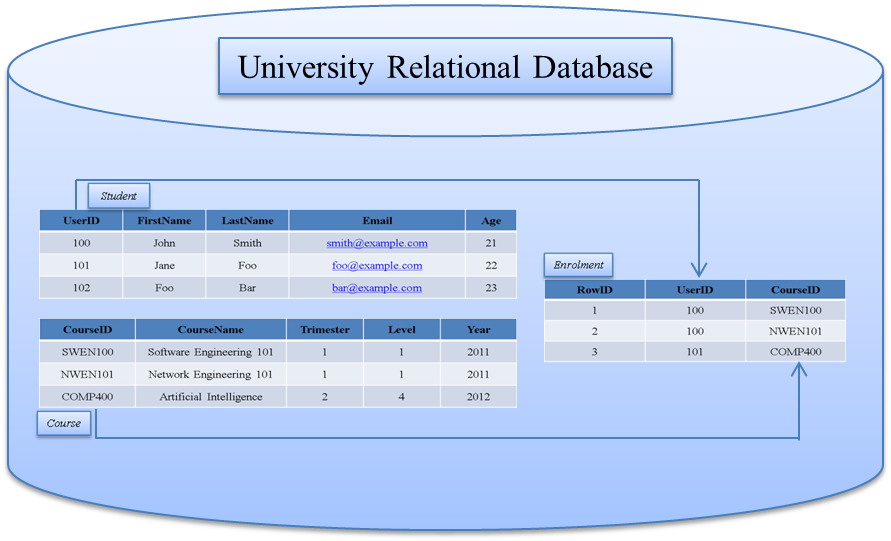
\includegraphics[width=.8\textwidth]{./figure/Example/Relational-DB.png}
	\caption{University example as a Relational database}\label{f:RDB}
\end{figure}

This shows how the University database example is deployed as a
\ac{RDB}.  When data in the University example is modelled using the
column-oriented key-value data model,   the way it is stored is different. 
Although key-value \acp{DBMS} are schema-less,   column-oriented key-value
\acp{DBMS} are not entirely schema-less and hold fewer information about the
constraints within the databases as metadata ,   as seen in Cassandra
(\todo{cite DataStax}).  This data model allows
applications to model the way data is organised in a traditional RDBMS whilst
bringing more flexibility by denormalising data and imposing no rigid structures
or schema requirements (\todo{cite DataStax}).  Therefore,   it allows
applications to add data in the way they want and change their schema (if
needed),   without adhering to a rigid
schema unlike the traditional \acp{RDBMS}.

The building blocks of column-oriented key-value databases are the columns,  
the Super Columns,   the Column Family and the Key Space.  Using the
University example,   these terminologies are explained below. 
Appropriate analogies are drawn with the \ac{RDB} University,   as
seen in Figure~\ref{f:RDB},   to better understand these column-oriented key-value
concepts.  Since the focus is on Cassandra's data model,   these concepts
are explained in the way Cassandra deploys them.  The example used
to describe the Cassandra data model adopts a simple and flexible schema that
allows some structure in the way data is stored. 

\begin{description}
\item[Columns:]  A column is the basic unit of data in this data model.  It is a
tuple containing a column name,   a value and a timestamp (Figure~\ref{f:column}). 

\begin{figure}[h]
	\centering
	%\includegraphics[width=5cm,   height=5cm]{. /figure/random. jpg}
	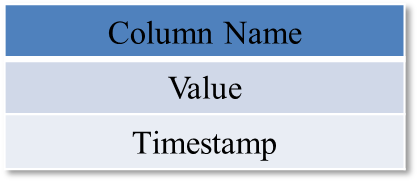
\includegraphics[width=.4\textwidth]{./figure/Example/Column.png}
	\caption{Random Pic}\label{f:column}
\end{figure}

The column names are labels  and it is mandatory that a column has a
name.  Column names and values are stored as Bytes Type,   Long Type,  
Ascii Type,   binary values Lexical UUID Type,   Time UUID Type or as UTF8
serialized strings (\todo{cite }).  Timstamps are used to store the time of the
latest update made to the column and are thus used for conflict resolutions.  The
timestamp values are commonly stored as microseconds,   but could be in any format
that the application chooses.  However,   timestamp formats have to be consistent
across the database so that is the same format across all columns. 

Cassandra allows indexes to be created on column names.  These are called
Secondary indexes and are of type \texttt{Keys} in Cassandra.  When such secondary indexes
are used,   efficient queries can be specified using equality predicates,   and
can be made on ranges of columns too.  The latter ones are called range queries. 

A column name can be considered analogous to a column
in a table in any traditional \ac{RDBMS}.  To illustrate this analogy,
Figures~\ref{f:column-FirstName} and~\ref{f:RDB-User} show the differences
between the representation of values in \texttt{Student} in Cassandra and in an
\ac{RDBMS}.
It can be seen from these figures that a column in the column-oriented key-value
data model is similar to a single value in a row of a relational table.  For
example,   the data '\texttt{John}' in the relational table \texttt{Student} can
be considered equivalent to a single column in Cassandra.

\begin{figure}[H]
	\newcommand{\W}{.4\textwidth}
	\centering
	%\includegraphics[width=5cm,   height=5cm]{. /figure/random. jpg}
	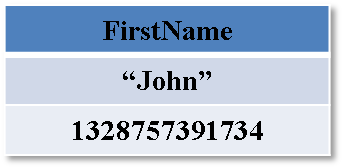
\includegraphics[width=\W]{./figure/Example/Column_FirstName.png}
	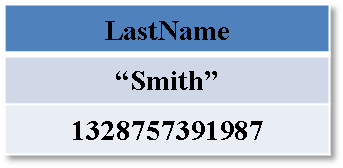
\includegraphics[width=\W]{./figure/Example/Column_LastName.png}
	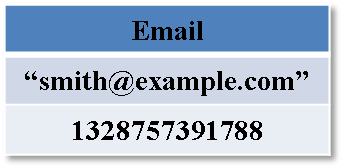
\includegraphics[width=\W]{./figure/Example/Column_Email.png}
	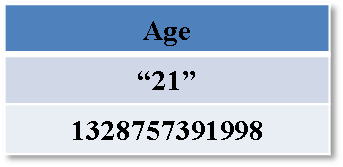
\includegraphics[width=\W]{./figure/Example/Column_Age.png}
	\caption{Columns in Cassandra}\label{f:column-FirstName}
\end{figure}

\begin{figure}[h]
	\centering
	%\includegraphics[width=5cm,   height=5cm]{. /figure/random. jpg}
	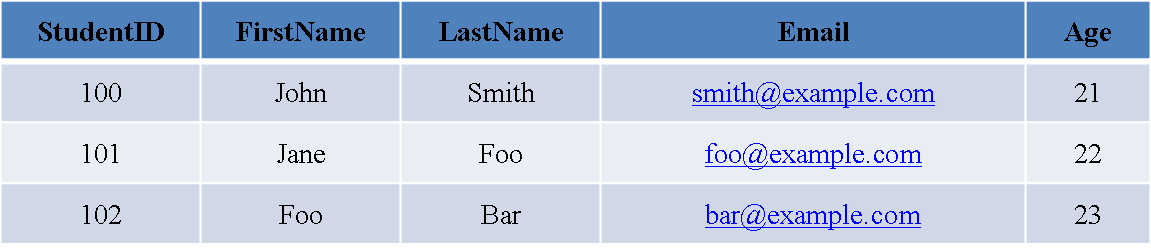
\includegraphics[width=.8\textwidth]{./figure/Example/RelationalTable_User.png}
	\caption{Relational Table - Student}\label{f:RDB-User}
\end{figure}

The JSON notation for  columns in Cassandra is shown in Figure~\ref{f:column-JSON}. 

\begin{figure}[H]
	\centering
	%\includegraphics[width=5cm,   height=5cm]{. /figure/random. jpg}
	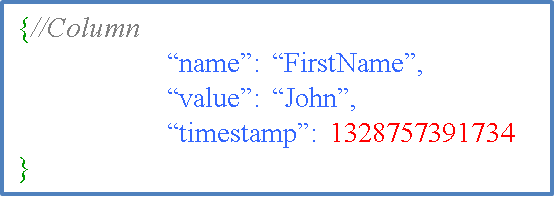
\includegraphics[width=.4\textwidth]{./figure/Example/Column_JSON.png}
	\caption{JSON notation for a column}\label{f:column-JSON}
\end{figure}
% 
% Alternatively,   applications can also use column names to store values.  This is
% possible since it is not required that columns always have values and
% since column names are byte arrays,   applications can store any kind of
% values in it. 

\item [SuperColumns:] A super column is a different kind of a column where the
values are an array of regular columns (Figure~\ref{f:supercolumn}).  It consists of a super
column name and an ordered map of columns.  The columns within the values of a
super column are grouped together using a common look-up value,   which is
commonly referred to as the \texttt{RowKey}.  In other words,   a super column is a
nested key-value pair of columns.  The outer key-value pair forms the super column while the inner
nested key-value pairs are the columns.  Unlike regular columns,   super columns do
not have timestamps for its key-value pairs.  

\begin{figure}[H]
	\centering
	%\includegraphics[width=5cm,   height=5cm]{. /figure/random. jpg}
	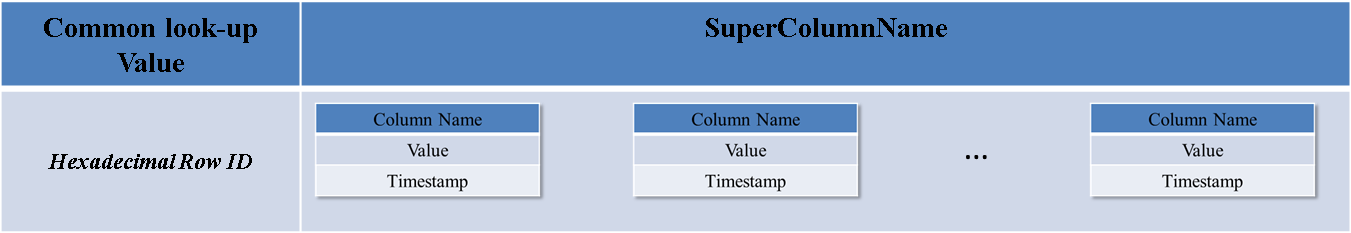
\includegraphics[width=.8\textwidth]{./figure/Example/SuperColumn.png}
	\caption{A Super Column }\label{f:supercolumn}
\end{figure}

A super column can be considered roughly similar to a whole record in a
relational table in an \ac{RDB}. For example,   the super column for a
student,   as seen in Figure~\ref{f:supercolumn-John},   is analogous to a single
record in the relational table \texttt{Student} (Figure~\ref{f:RDB-User}). 

\begin{figure}[H]
	\centering
	%\includegraphics[width=5cm,   height=5cm]{. /figure/random. jpg}
	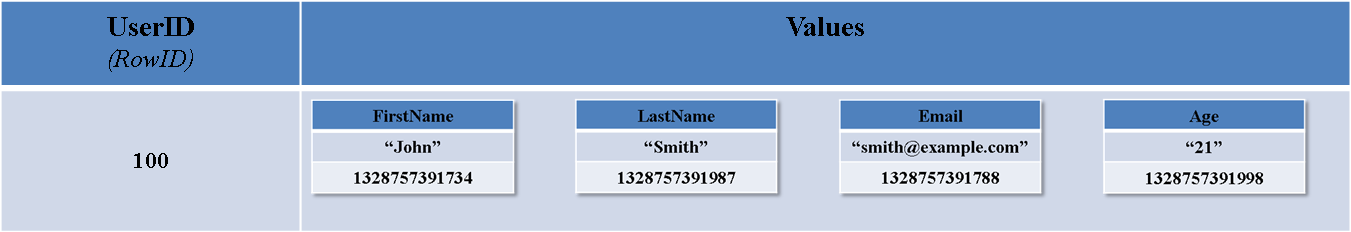
\includegraphics[width=.8\textwidth]{./figure/Example/SuperColumn_John.png}
	\caption{A Super Column for Student '\texttt{John}' in
	Cassandra}\label{f:supercolumn-John}
\end{figure}

The JSON notation for a super column is shown in Figure~\ref{f:supercolumn-JSON}. 

\begin{figure}[H]
	\centering
	%\includegraphics[width=5cm,   height=5cm]{. /figure/random. jpg}
	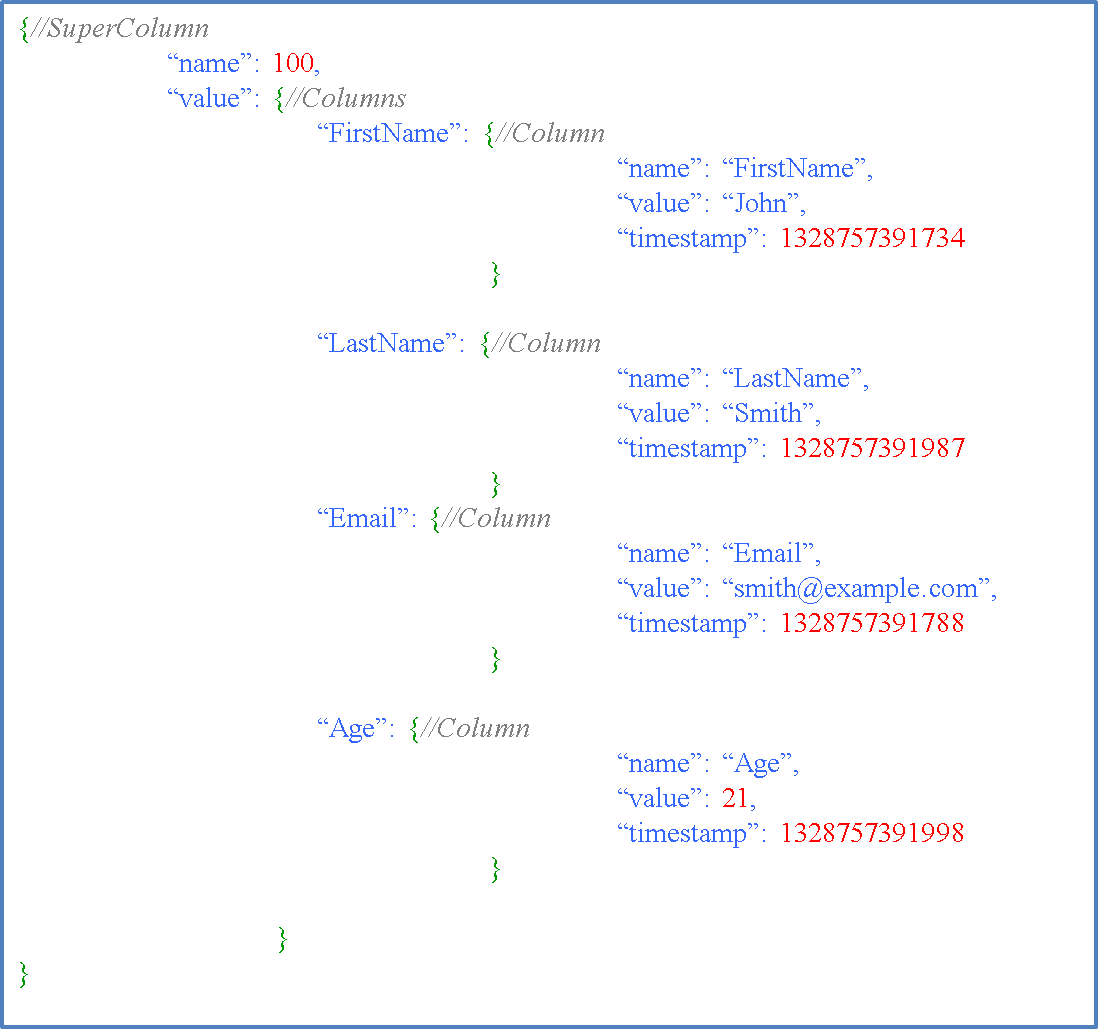
\includegraphics[width=.7\textwidth]{./figure/Example/JSON_SuperColumn_John.png}
	\caption{JSON notation for a super column}\label{f:supercolumn-JSON}
\end{figure}

\item [ColumnFamily:] A column family contains columns or super columns that are
grouped together using a unique row key.  It is a set of key-value
pairs,   where the key is the row key and the value is a map of column names
(Figure~\ref{f:columnfamily}).  The row key groups the columns together,   just as
in super columns. 

\begin{figure}[H]
	\centering
	%\includegraphics[width=5cm,   height=5cm]{. /figure/random. jpg}
	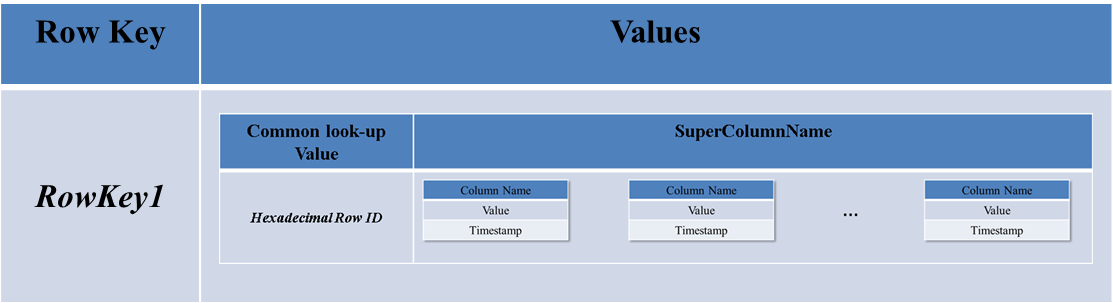
\includegraphics[width=.8\textwidth]{./figure/Example/ColumnFamily.png}
	\caption{Column Family in Cassandra}\label{f:columnfamily}
\end{figure}

Applications can define column families and metadata about the columns. 
It is commonly practised to have columns that are related or accessed
together to be grouped in the same column family.  Column families require that
some attributes are always defined,   like name,   column type and others.  It
also has optional attributes that can be defined if the application requires so.
 Some of the optional attributes are number of keys cached,   comments,   read
repairs,   column metadata among others.

Column families can have rows %to have relatively a definite number of columns. 
that are identified by their unique row keys.  This is similar to a table,   as
seen for table \texttt{Student} in Figure~\ref{f:RDB-User},   where every row in
the table has the same number of columns and primary keys are used to identify a
row.  An example of a column family is shown in Figure~\ref{f:columnfamilyUSER}.
Unlike relational tables in an \ac{RDB},   column families do not require all
the rows to define the same number of columns (\todo{cite Sarkissian}).

\begin{figure}[H]
	\centering
	%\includegraphics[width=5cm,   height=5cm]{. /figure/random. jpg}
	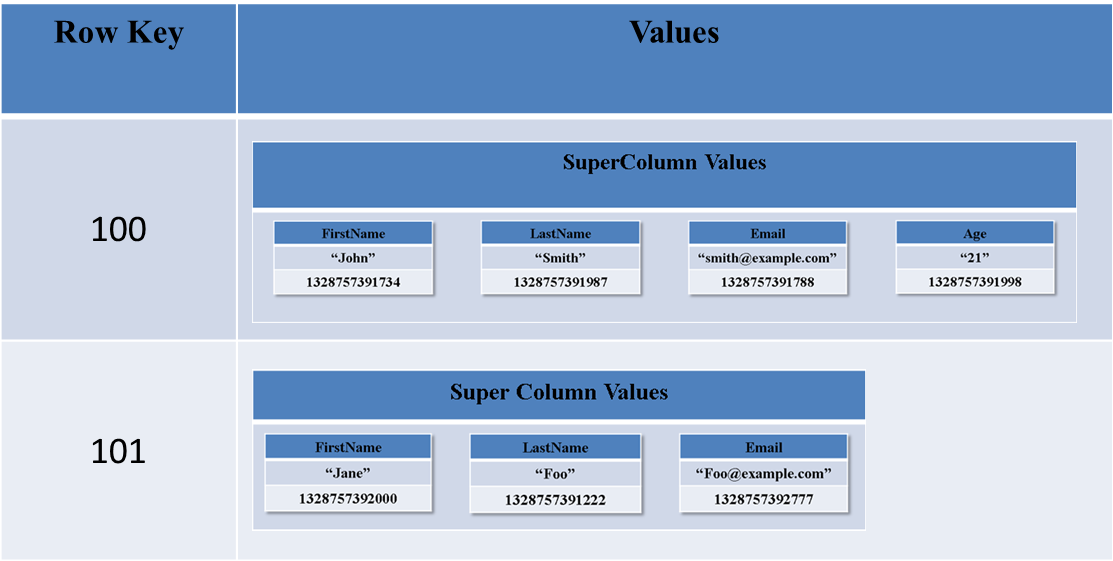
\includegraphics[width=.8\textwidth]{./figure/Example/ColumnFamily-User-DiffColumns.png}
	\caption{Column Family \texttt{User} in Cassandra}\label{f:columnfamilyUSER}
\end{figure}

The JSON notation for a single row of a column family in Cassandra is
shown in Figure~\ref{f:columnfamilyJSON} 

\begin{figure}[H]
	\centering
	%\includegraphics[width=5cm,   height=5cm]{. /figure/random. jpg}
	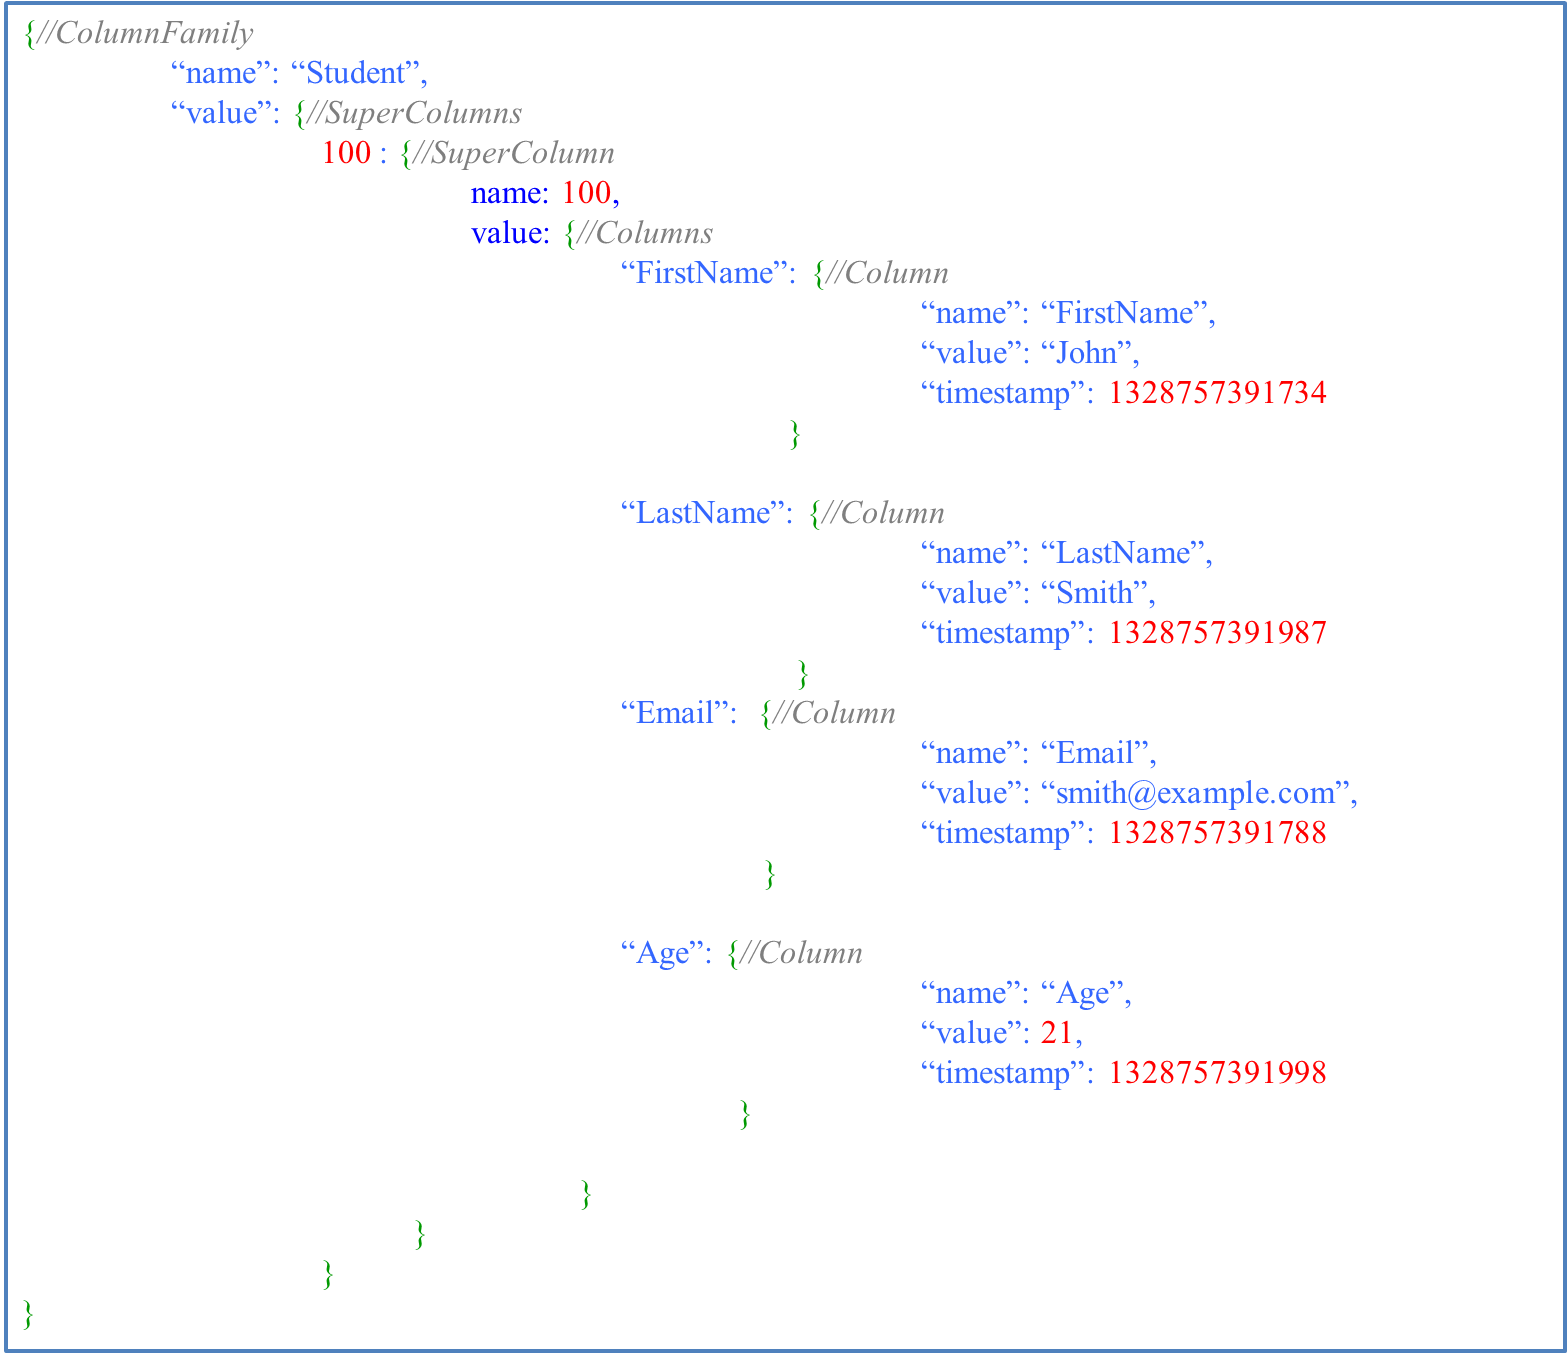
\includegraphics[width=.8\textwidth]{./figure/Example/JSON_ColumnFamily_1row.png}
	\caption{JSON notation for a column family in
	Cassandra}\label{f:columnfamilyJSON}
\end{figure}

\item [KeySpace:] A keyspace is a container to hold the data that the
application uses.  Keyspaces have one or more column families,   although it is not strictly
required that a keyspace should always have column families.  Any relationships
existing between column families in a keyspace are not preserved. 

A keyspace can be considered similar to a database in traditional relational
databases,   without any relationships.  An example of the keyspace
University is shown in Figure~\ref{f:keyspace}. 

Keyspaces require that some attributes are defined,   like a user defined name,  
replication strategy and others.  Some optional elements that can be defined are
the details of the column families in the keyspace and other options
for replication of data. 
\end{description}

%\newpage

\begin{figure}[H]
	\centering
	%\includegraphics[width=5cm,   height=5cm]{. /figure/random. jpg}
	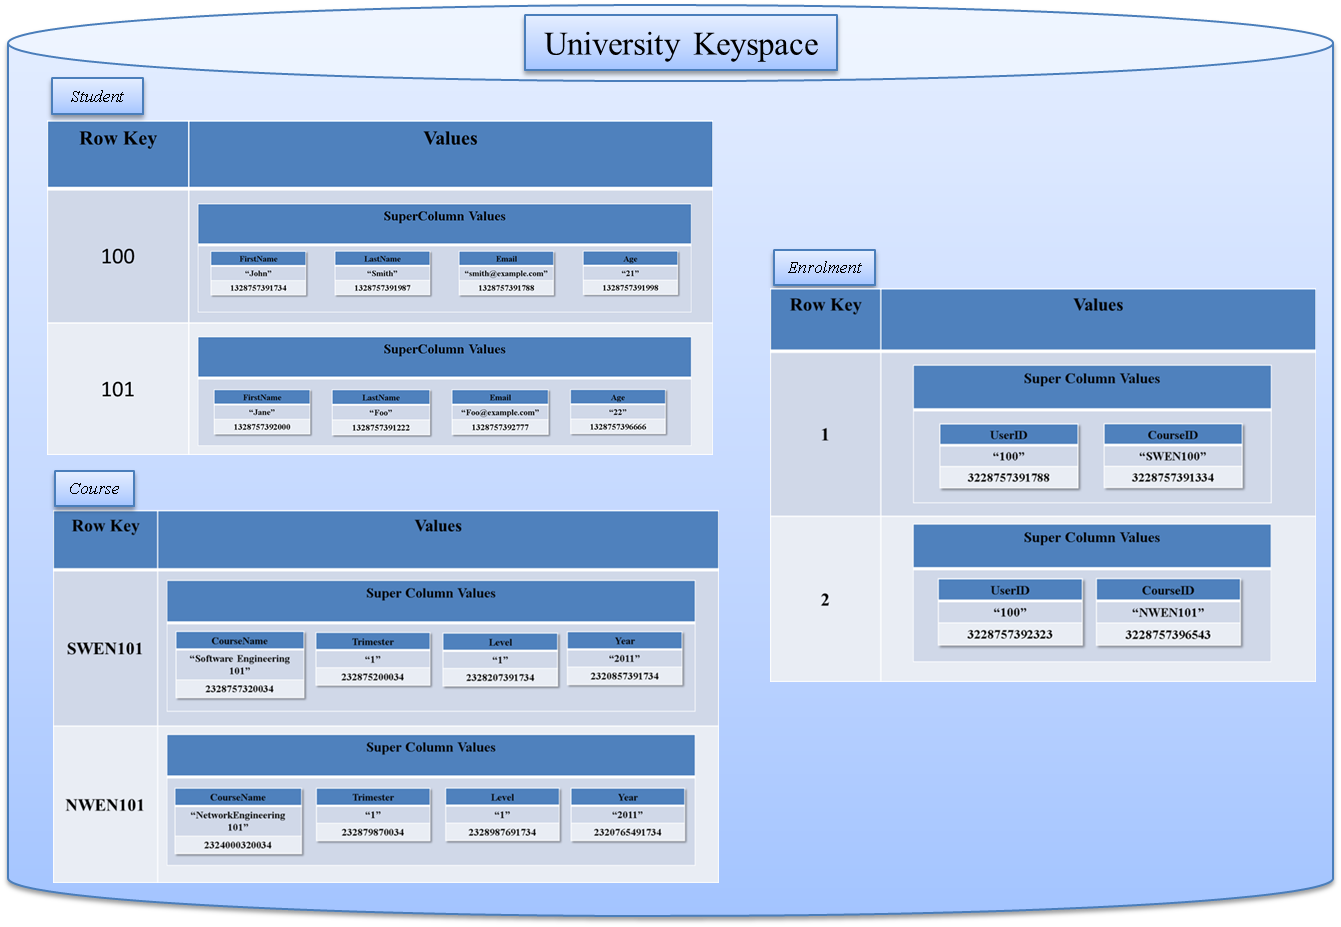
\includegraphics[width=.9\textwidth]{./figure/Example/KEYSPACE.png}
	\caption{A keyspace in
	Cassandra}\label{f:keyspace}
\end{figure}

As previously mentioned,  cloud \ac{NoSQL}
\acp{DBMS} are generally specialised to address specific problems like
partition-tolerance,  high availability among others and for this some
trade-off are made when these are developed.
Some of the challenges and problems present in such \acp{DBMS} are discussed in the following section.

\section{Challenges in Key-Value model}\label{s:challenges-key-value}
Fundamentally,   the key-value data model is different from the relational model
in many ways.  While the relational data model aims at giving data a structure,  
providing data integrity,   the key-value data model just
store data as \acp{blob} or string values and generally do not maintain
relationships between data.  In the column-oriented key-value model,   the
key-value association and the grouping of columns in column families can be
considered as the minimum relationship that is maintained.  

According to Bell and Brockhausen (1995),   data dependencies are the most
common types of semantic constraints in relational databases and these determine
the database design.  Data dependencies are the various relationships that may
exist between data entities in a database.  For example,   in the
University database,   a student can enrol into more than one course and this
means that there is a many-to-many relationship between \texttt{Student} and
\texttt{Course} since   one course can have many students enrolled in it.  

As seen in Section~\ref{s:key-value-data-model},   the \texttt{Enrolment} table 
contains the \texttt{StudentID} and the \texttt{CourseID} as foreign keys,  
thus showing the dependency or relationship between students and courses
(Figure~\ref{f:RDB}). 
In the \texttt{University} \ac{RDB} any attempt to delete a course
from the \texttt{Course} table,   is prevented by a constraint,   unless the
dependency itself is removed first.  In \acp{RDBMS} ,   this constraint is referential
integrity,   which ensures that references between data entities are valid,  
consistent and intact (\todo(cite Blaha,   n. d. )). 
Normalisation,   as well as modelling real world data and
relationships enforce such dependencies in the schema and this causes integrity
constraints like referential integrity constraints,   to be imposed on data
entities. 

If such constraints are not imposed,   there could arise many dangling
dependencies in the database.  For instance,   consider the case of foreign key
references between \texttt{Course} and \texttt{Enrolment} in the  University
database.  If a course is deleted from the \texttt{Course} table without removing
its dependencies in \texttt{Enrolment},   the latter would contain active references
to the deleted course.  Another example of a dangling reference occurs during
insertion of data,   where a new student is entered in the
\texttt{Enrolment} table,   with a \texttt{CourseID},   that does not
exist in the \texttt{Course} table (i. e. ,   wrong \texttt{CourseID}).  A dangling
reference occurs because this inserted student refers to a nonexistent course. 
Such problems cause inconsistent data to be stored in databases and violate data
integrity.  To ensure that users get consistent and valid information,  
applications would have to implement mechanisms to check or prevent dangling references.  But if
referential integrity constraints are applied as in an \ac{RDB},   operations
on data that  adversely affects referential integrity   would not be
permitted.

As previously mentioned,   \ac{NoSQL} database systems do not normalise data and
nor are any relationships maintained.  But relationships or dependencies
between data are common when real world data is stored in databases.  For example,   in the
real world,   a course could be taught by more than one lecturer or a student with
an Art major is restricted entry into Chemistry courses etc.  These relationships
and constraints have to be preserved upon storage in
cloud \ac{NoSQL} database systems too.  As mentioned in
Section~\ref{s:cloud-databases},   cloud databases,   whether relational or
\ac{NoSQL},   have to replicate data across several machines and need to be
scalable to match the needs of the users.  The replicated and distributed nature
makes maintaining data dependencies complex and unfeasible in terms of speed and
efficiency.  In cloud \ac{NoSQL} databases,   this effectively means that the
relationship between \texttt{Enrolment}, \texttt{Student} and \texttt{Course}
tables will not be strictly enforced and deleting a course in cloud \ac{NoSQL} databases is allowed because
of the absence of constraints.  As mentioned before,   this means that students
could still be enrolled in deleted courses,   since there are no constraints to
prevent such deletions or changes in cloud \ac{NoSQL} databases. 

Commonly,   developers impose such constraints and reference checks on \ac{NoSQL}
data at the application side.  Another way to implement such checks is to give
these constraints at the persistence layer of the application server.  Both these
ways would eventually have to handle all the processing and managing of these
constraint checks for all the widely spread data in \ac{NoSQL} databases. 
However,   this could mean immense workload on the application or the application
server,   especially if the data volume is large in the \ac{NoSQL} database or if it is
has many replicas that have to be checked as well for the constraints. 


This is a serious problem when data is interconnected and dependant on other
data entities as is commonly the case.  For example,   consider a banking
application that uses cloud \ac{NoSQL} \acp{DBMS} where its data is spread
across several nodes and is interconnected.  Any debit or credit
transactions made to a users account will have to be replicated across all the
nodes and correctly persisted.  Many constraints will exist for transfer of funds
between user accounts and such constraints need to be validated correctly.  If a
user has multiple accounts,   the relationship between the accounts have to be
maintained too.  When such constraints are not validated correctly,   it will lead
to incorrect account balances and wrong updates in the user accounts.  On the
other hand,   when such applications use an \ac{RDBMS},   referential integrity
constraints would be imposed to maintain the relationships between the
accounts and such constraints would be defined while tables are created and
their validation would be triggered whenever any operations are performed on the
data. 

Updates may not be correctly reflected across all the nodes of the database due
to  eventual consistency too,   which is discussed in Section~\ref{s:Cassandra}. 
However, in spite of eventual consistency,   data dependencies should be correctly handled and
recorded. 

Although such problems mostly affect most cloud \ac{NoSQL} \ac{DBMS} users,   it
could be different for different users.  For example,   a banking system as
mentioned above could be gravely affected because of dangling references while
in a simple game application such problems could be trivial. 

% Motivated by such problems of data dependencies,   this thesis studies the
% existing modelling of data dependencies in cloud \ac{NoSQL} database systems and
% aims to contribute by suggesting four solutions so that referential integrity
% is effectively maintained,   while also not limiting the benefits of not having
% a rigid schema in \ac{NoSQL} database systems.  Such a result would reduce the
% workload of the applications or the persistence layers of the application
% servers.  Additionally it would give users of \ac{NoSQL} database systems
% better consistency in data,   along with ensuring better data integrity even when
% it is widely replicated or spread on different data-centers. 



\section{Referential Integrity in Key-Value
Model}\label{s:referential-integrity}
Addressing the aforementioned challenges,   implies to introduce referential
integrity constraints in cloud \ac{NoSQL} database systems. 

Referential integrity is a fundamental property of data within databases,   which
ensures that data dependencies between tables are maintained correctly in the
database (\todo{cite oracle}).  These dependencies could be a part of the
business rule and need to be enforced for proper data integrity.  Users define
conditions or rules on the tables in a database so that data integrity is
ensured at all times.  These conditions are called integrity constraints and need
to be mandatorily satisfied at all times in order to ensure that users or
applications do not enter incorrect or inconsistent data into the databases. 

The Referential Integrity Constraint is just one amongst other constraints,   and
generally in \acp{RDBMS},   these constraints ensure that the value of foreign
keys in a table matches the values of primary keys in another table.  The table
containing the foreign key is the referencing table (or child table),  
while the table with the primary or unique key is the referenced table (or parent table). 
For example,   in the University database,   \texttt{Enrolment} is the
referencing table while \texttt{Student} and \texttt{Course} are the
referenced tables.  Foreign keys are also known as the referencing key and
the primary keys as the referenced keys. 

It has been defined by many researchers that referential integrity is enforced
by the combination of a primary (or unique) key and a foreign key,   and that
every foreign key has to match the primary key (\todo{cite}).  In the
University example,   every foreign key in the \texttt{Enrolment} table must match
one of the primary keys in the \texttt{Student} and \texttt{Course} tables. 
Hence,   if any foreign key refers to a non-existing primary key,   the
referential integrity constraint is violated.   For example,   if
'\texttt{StudID100}' is a foreign key for a student in the \texttt{Enrolment}
table,   but '\texttt{StudID100}' does not exist as a primary key in the \texttt{Student}
table,   then it is a violation of referential integrity. 
 
Referential integrity constraints also describe the data manipulation that is
allowed on the referenced values.  Some of the widely associated rules are:

\begin{itemize}
  \item \texttt{Restrict} or \texttt{No delete}: which prevents any update or
  deletion of data that has references. 
\item \texttt{Set to NULL}: which sets all foreign keys to NULL values,   on
updating or deleting the referenced key. 
\item \texttt{Set to Default}: which sets all the foreign
keys to a default value,   on updating or deleting the referenced key. 
\item \texttt{Cascade}: which updates or deletes all the
associated dependant values accordingly,   when the referenced data is updated or
deleted. 
\item \texttt{No Action}: which performs checks only at the end of a
statement and is similar to \texttt{Restrict}
\end{itemize}

Existing \acp{DBMS} may not always support all of the above rules.  Some \acp{DBMS} may
have the \texttt{Cascade} rule by default like Oracle,   while some may have the
\texttt{Restrict} rule by default.  

Generally,   in \acp{RDBMS} the database manager enforces a set of rules to
prevent nay data operation,   like insert,   update or delete,   to change data in
such a way that referential integrity is not violated as seen in
Figure~\ref{f:RI}. 

\begin{figure}[H]
	\centering
	%\includegraphics[width=5cm,   height=5cm]{. /figure/random. jpg}
	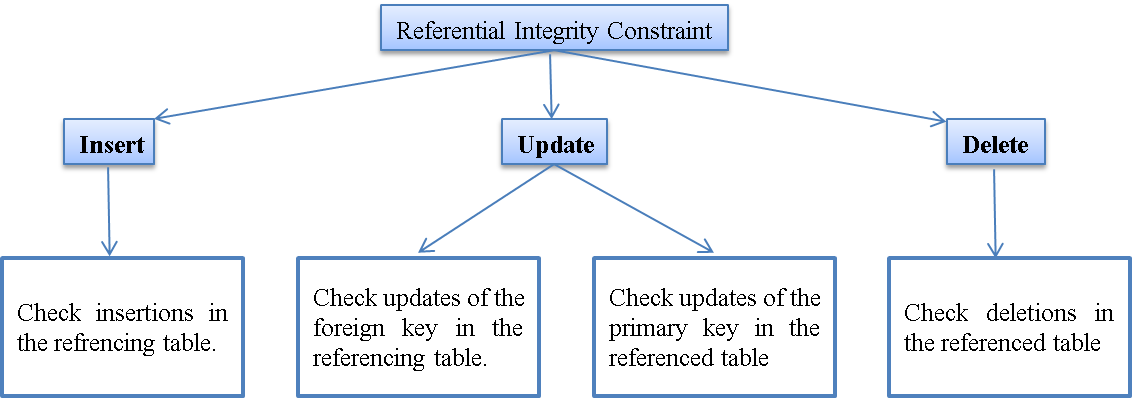
\includegraphics[width=.8\textwidth]{./figure/Example/RI-Figure.png}
	\caption{Referential Integrity Rules}\label{f:RI}
\end{figure}

These rules are explained below:

\begin{itemize}
  \item Insert rule: An insert operation triggers a referential integrity
validation when data is being inserted into a referencing table,   i. e. ,   the
child table.  In such an event,   prior to entering the values in the referencing
table,   it is checked if the foreign keys exist in the referenced table.  For
example,   in the University \ac{RDB},   when a row is inserted in the
\texttt{Enrolment} table with foreign key values for \texttt{StudentID} and
\texttt{CourseID},   a check is triggered to verify whether these foreign keys
exist in the \texttt{Course} and \texttt{Student} tables as primary keys.  If
the foreign keys do not exist in the referenced tables,   then the insert operation is not allowed. 

\item Update rule: When data is updated either in the referencing table or
the referenced table,   a referential integrity validation is needed.  When any
primary key is updated in the referenced table,  
then it is verified whether this key is a foreign key in any of the
referencing tables.  If a dependency is found to exist,   then the applicable
data manipulation rule is checked.  For instance,   if it is a \texttt{Cascade}
rule,   then the associated foreign keys in the referencing table are updated
prior to updating the key in the referenced table.  In the University \ac{RDB},  
if the primary key '\texttt{SWEN100}' for a course is updated to
'\texttt{SWEN101}',   then all the records in \texttt{Enrolment} that have
'\texttt{SWEN100}' as a foreign key have to be updated to '\texttt{SWEN101}',  
if it has a \texttt{Cascade} rule. 

When any foreign key is being updated in a referencing table,   then a referential
integrity validation has to be performed.  It is ensured that the new
updated value exists as a primary key in the referenced table.  For example,   in
the \texttt{Enrolment} table,   if \texttt{CourseID} in a row is updated to a new
value,   then it is verified that the new value is an existing primary key in the
\texttt{Course} table.  If the new value does not exist,   the
update is not allowed generally. 

\item Delete rule: A delete operation triggers a referential integrity
validation when data is deleted from the referenced table.  When data that is marked
for deletion is found to have dependencies in other referencing tables,   the
data manipulation rule applicable for this operation has to be checked.  This
means that if the rule allows \texttt{Cascade},   then the depending values in the
referencing table have to be removed prior to deleting values from the
referenced tables.  For example,   when a student record is deleted from the
\texttt{Student} table,   a check is performed to see if the '\texttt{StudentID}'
is a foreign key in any other table.  Therefore,   \texttt{Enrolment} would be
checked and when the '\texttt{StudentID}' is found as a foreign key,   the
appropriate action is performed depending on the data manipulation rule.  If it
is '\texttt{Cascade}',   the enrolment details for the '\texttt{StudentID}' are
removed from \texttt{Enrolment} and then the student record is deleted from
\texttt{Student}. 

\end{itemize}

Referential integrity constraints have been a relational feature in traditional
\acp{RDBMS} and is imposed due to the way the \acp{RDBMS} enforce normalisation. 
To improve the data dependency in cloud \ac{NoSQL} \acp{DBMS},   this
thesis proposes solutions that implement referential integrity constraints using
different approaches. These solutions implement and
validate referential integrity constraints based on these fundamental data manipulation and
referential integrity rules and are discussed in Chapter 3.

% These proposed solutions are deployed and analysed in Cassandra,  which is a
% column-oriented key-value \ac{DBMS}. To implement any solution it is necessary
% to understand the architecture and the key operations allowed in a \ac{DBMS}.
% For this purpose,  the architecture of Cassandra is discussed in the following section.



\section{Summary}



This chapter presented the background about the underlying concepts in cloud
computing and cloud databases.  It is clear that cloud computing is gaining
prevalence due to its many benefits like high data availability and cheap
storage etc.  With an increase in the number of users
migrating to cloud computing,   cloud data storage is gaining prominence as well,  
for easy and simple data storage.  This has paved the way for the existence
of many different data models and databases on the cloud.  Amongst the many data
models,   the key-value data model has been  most widely used  on the cloud
as it is more adapted to the cloud environment due to its support for
replication and scalability and other cloud related features (\todo{cite}). 



The next chapter describes the four solutions proposed to enforce referential
integrity constraints in cloud \ac{NoSQL} \acp{DBMS},   particularly in
Cassandra which is based on the column-oriented key-value data model. 





 
% %ब
\section{Apache Cassandra} \label{s:Background-Cassandra}

Cassandra is a distributed data storage system initially developed by Facebook
for satisfying the needs of large web applications that handle large
volumes of data~\citep{BOOK}. 
Its development has been undertaken by Apache  and it is  currently used by
many large web applications and large organisations like Facebook,  Twitter, 
Cisco,  Digg,  Reddit, and others~\citep{datastaxB}. 

Cassandra is based on the column-oriented key-value data model and stores data
as columns,  super columns,  column families and keyspaces, all of which are
explained in Section~\ref{s:key-value-data-model}. Being a distributed
system, Cassandra can run on multiple machines 
% runs as a single Java process on each machine in a cluster.
and provides the option  to work across different machines and across
multiple data centers,  even if these  are geographically
distributed~\citep{BOOK}.
These machines  are configured to operate together and
run as a single cluster, where these
% the entire cluster behaves like a unified whole. and access to only
% one of the nodes is required to perform operations.
 machines form a ring of nodes~\citep{datastax,BOOK}. Such
nodes are connected to each other and each node is aware of all their peers in
the cluster (Figure~\ref{f:cassandra-cluster}).


\begin{figure}[h] \centering 
	% \includegraphics[width=5cm,    height=5cm]{.  /figure/random.  jpg}
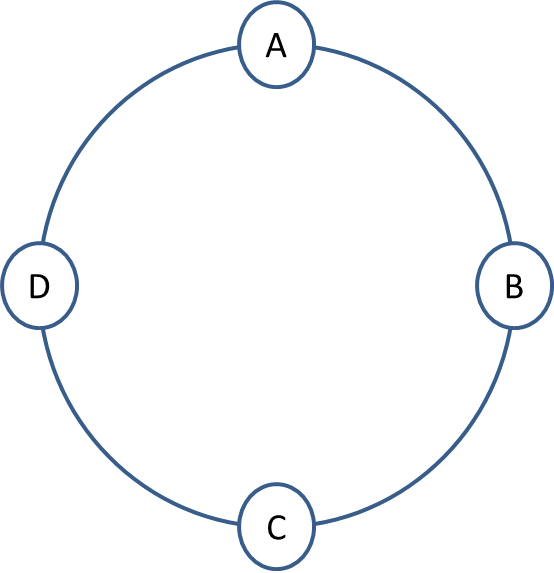
\includegraphics[width=.3\textwidth]{./figure/Background/CassandraCluster.png}
	\caption{A cluster of nodes in Cassandra}\label{f:cassandra-cluster}
\end{figure}

The nodes in a cluster communicate with each other to send their state
information at regular time intervals,  so that other nodes in the ring  know
their status~\citep{BOOK,cassandra}. Such communication
between the nodes support failure detection in Cassandra as when
% helps in failure detection in Cassandra since
 a node fails,  it stops responding to messages from other
active nodes and in this way the rest of the nodes  know of its inactive state.
% Cassandra is fault tolerant and able to perform operations despite node
% failures.
% Even when some parts of the cluster are inactive, Cassandra is fault tolerant
% and contiune performing its operations. 
In the event of a node failure,
operations sent to it are not lost since another active node ensures these are
performed~\citep{cassandra}.

In such a cluster,  every node applies the same architectural features
fundamental to Cassandra,  namely,  load balancing,  replicating
and partitioning data,  failure detection mechanisms, among others.  Some of the
key architectural concepts of Cassandra are explained next. 

% Distributed system are prone to conflicts as many users could be issuing
% requests on data items from any of the nodes.  Any distributed system should
% carefully consider conflict resolution and adopt design approaches which would
% resolve such conflicts efficiently.  Conflicts arise either at read or write
% operations. 
% The design approach should either make the system resolve such conflicts either
% during one of these operations,  deciding the system be either readable at all
% times or writable.  Cassandra optimises its performance by adopting the design
% approach of resolving conflicts during read operations,  making Cassandra always
% writable. 



\subsection{Architecture} \label{ss:Background-Cassandra-Archi}
Cassandra adopts many of its  architectural concepts from other popular
distributed key-value data storage systems on the cloud,  like Google's Bigtable
and Amazon's Dynamo~\citep{ycsb,Dynamo}.  Over time, these adopted concepts
evolved and developed new features,  some of which became specific to Cassandra's
architecture. Some of these  concepts are, peer-peer distribution model, data
partitioning, eventual consistency, among others. These  concepts gave Cassandra
  features such as elastic scalability,  fault tolerance, high availability and
high performance.
% Cassandra's architecture involves many sophisticated and complex theoretical
% as well as mathematical concepts,
% Following are some of the key architectural concepts of Cassandra.
% Discussing every concept is beyond the scope of this research.

\vfill

\subsubsection{Peer-Peer Distribution Model}
% Generally,  in traditional distributed
% \acp{DBMS},  nodes in a cluster are configured to have different
% responsibilities and roles where some or one of the nodes is a master and others
% are slaves.  Such a centralised configuration improves reading data,  as data can
% be read from any of the slave nodes,  but write requests are always sent to the
% master node.  This model thus puts a lot of additional load on the master and
% also is prone to failure if the single master node is offline.  However, 
Cassandra is a decentralised system  where all the nodes are considered equal
or identical (i.e.  nodes are peers) in sharing responsibilities and performing
operations,  without any  master or slave nodes~\citep{datastaxB,BOOK}. 
This model provides high data availability since failure
of a node does not affect the service of the cluster  because other
nodes carry out the same operation. 
% Moreover,  when new nodes are added to a cluster there is no additional task of
% delegating responsibilities or roles since all the nodes have the same
% responsibilites. 

% The nodes in a cluster communicate with each other to send their state
% information at regular time intervals,  so that other nodes in the ring can know
% their status (\todo{cite Cassandra paper}).  This helps in failure detection in
% Cassandra since if a node is not active it fails to send or respond to  messages
% from other active nodes and in this way the rest of the nodes  know of its
% inactive state.  In the event of a node failure,  another active node  performs
% the operations in order to ensure that  operations that were sent to a failed
% node are not lost (\todo{cite Cassandra papers}). 
% The recepient node  creates a small hint message with the information about
% the operation so that it can give the hint to the failed node once it is
% alive again and this feature is called hinted handoff. 

\subsubsection{Data Partitioning}
Cassandra partitions data between the nodes in a cluster  so that data items
from overloaded or failed nodes are assigned to other nodes or new nodes.  For
this,  Cassandra uses consistent hashing where data items are hashed on its key.
After hashing the key, the data items are assigned to the node whose
position in the ring is larger than the hashed value of the key~\citep{BOOK}.
% used by Amazon's Dynamo to partition data over the nodes. (\todo{DeCandia et
% al. (2007)}). 
% \begin{figure}[h] \centering %\includegraphics[width=5cm,    height=5cm]{. 
% /figure/random.  jpg}
% 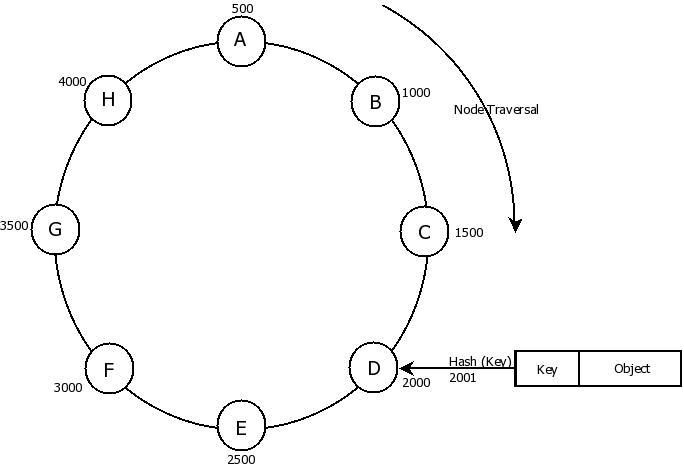
\includegraphics[width=. 6\textwidth]{. /figure/Cassandra/Consistent-hashing-Cassandra. png}
% \caption{Consistent hashing in Cassandra}\label{f:consistent hashing}
% \end{figure}
Data partitioning makes Cassandra elastically scalable since the load is
balanced and distributed in the cluster  irrespective of addition or removal of
nodes~\citep{BOOK,cassandra}. 
% Additionally,  in Cassandra better performing nodes are assigned multiple
% points in the ring,  making them virtual nodes and these nodes are assigned
% workloads from failed nodes or overloaded nodes. 

\subsubsection{Replication strategy} In order to ensure high data availability
irrespective of failures,  Cassandra uses a replication strategy where every
data item is replicated across a number of nodes.  Applications can set the
level of replication to suit its requirements,  that is, the replication factor
is set to the number of nodes on which the application wants to create
replicas~\citep{BOOK,cassandra}.  The
replication factor tells the cluster how many copies to create of a single data item.
Setting the replication factor to a large number will help in higher
consistency of data items,  but replicating data items to a large number of
nodes  can adversely affect the performance.

Once data items are partitioned and assigned to a node,  these are
replicated onto other nodes and a list of the nodes responsible for storing the
data items are maintained.  Thus, every node in the cluster knows which nodes
are responsible for a data item~\citep{BOOK,cassandra}.
Such a replication strategy makes data highly available  since data items can
be accessed from any node in a cluster regardless of node failures.  
% Since all
% the nodes  know which peer node is responsible for a data item,  
% routing requests to the correct nodes. 



\subsubsection{Eventual Consistency}
% As mentioned previously,  Cassandra opts for '\texttt{A}' and '\texttt{P}' of
% the CAP theorem and allows users to determine the level of consistency they
% prefer.  This consistency level tells the cluster how many replicas should
% acknowledge operations done on them,  for the replicas to be considered
% consistent and up to date.  Low consistency levels are considered better for
% performance as higher consistency levels involve more time since nodes have to
% wait to receive acknowledgements from more replicas.
% Letting the users decide the consistency level and replication factor means
% the tradeoff between consostency and performnace is detemined by the users.
In any strongly consistent  \acp{DBMS}, data items immediately reflect the new
values upon an insert or update operation. However, Cassandra uses the eventual
consistency model where replicas do not agree to the most recent value
immediately but will do so eventually. This is because the new values are
propagated to all the replicas in a cluster in an asynchronous
way~\citep{Tai,ycsb,henry,Vogel}.
% Eventual consistency provides Cassandra high scalability because any write or
% update operation  reaches all the replicas irrespective of the number of
% nodes in a cluster.
% Thus,  all replicas would be consistent eventually after a certain period of
% time, generally a small number of milliseconds \todo{cite book}.
% This is unlike strict consistency models  run on single nodes,  where a read
% operation always returns the most update values.
% In distributed systems like Cassandra,  several machines are used concurrently
% by many users leading to various conflicts,  which makes a weaker form of
% consistency like eventual consistency  ideal (\todo{cite BOOK and marked
% papers}).

 
\subsection{Write and Read Operations}
\label{ss:Background-Cassandra-Operations} 
In order to write data into Cassandra column families,  a write request is sent
to a random node in the cluster,  which acts as a proxy node and replicates the
data in the cluster~\citep{datastax,BOOK,cassandra}.
The number of nodes on which data is to be replicated can be changed to suit the
application requirements. Moreover, these nodes can be in the same data centre
and other data centres.

		

When a read request is issued to a node,  it acts as a proxy node and forwards
the request to all the other nodes in the cluster.
These nodes return their copy of the data item to the proxy node and the proxy
node  checks the versions of the replicas and sends the latest replica to the
user~\citep{datastaxRead}.   If the replicas received from a node are not
consistent with other replicas, a read repair is performed on the node
with the outdated replicas.  This means that the nodes with outdated replicas
are sent a write operation with the latest data.
Thus,  data consistency is maintained whenever conflicting versions of data
items are found.

When rows or columns are deleted in Cassandra, the  data within these rows or
columns is not removed immediately from the disk~\citep{datastax,BOOK}. Instead,
data is deleted after a time period that is configurable by applications. This
is called a tombstone delete in Cassandra, where the columns that are to
be deleted are only marked for deletion and empty values are written into such
columns.
Once the configured time period expires, the data is physically removed from the
disk. However, the row keys of the deleted columns continue to persist. Such a
tombstone delete is useful when a failed node is active again as this node can
update its replicas  correctly to show the deletions.



%  
% \acresetall
% %ब
\chapter{Design of Referential Integrity Constraints in NoSQL
databases}
\label{c:solutions}

% As mentioned previously,  cloud column-oriented key-value \acp{DBMS} lack
% referential integrity constraints to maintain foreign key relationships,  as
% seen in traditional \acp{RDBMS},  due to its non-relational data model. 
% Moreover,  these cloud \acp{DBMS} do not normalise data nor maintain
% relationships.
Traditionally, referential
integrity constraints are imposed on data items of a database to maintain
foreign key relationships. These relationships are
 maintained by correctly identifying and preserving the data dependencies 
 existing between the data items.
% Traditionally, foreign key relationships are
% maintained by correctly identifying and preserving the data dependencies existing between data items in a database.
% These dependencies are maintained and  validated by imposing referential
% integrity constraints on data items. 
Most popular traditional \acp{RDBMS}
preserve such dependency information in their \texttt{System} tables or data
dictionaries.  These tables store the necessary information  which is required
to maintain valid dependencies. The information stored in such tables include table
names,  primary and foreign keys among others.
This can be seen in popular \acp{RDBMS} like  MS SQL Server,  PostgreSQL,
Oracle, and so on.  

For example,  in MS SQL Server 2000, \texttt{sysforeignkeys}
is a \texttt{System} table which stores the information of all 
foreign keys of every table in a database, and \texttt{sysreferences}
stores the mappings of  foreign keys to the referenced primary key columns
(\todo{\citep{sys:msdn}}).
Information in these \texttt{System} tables consist of  the
names of tables and its constraints,  unique identifiers of 
referenced and referencing columns,  among others. 
In PostgreSQL, such information is saved as views which contain the dependency
information of data items in a database.
The view \texttt{table\_constraints} contains the information for all the
constraints in every table owned by the current user. (\todo{\cite{}}). 
Similarly, Oracle uses a \texttt{SYSTEM} meta-database to hold such constraint
information.
 In general, \texttt{System} tables or views with information
about the existing dependencies  are looked up by these \acp{RDBMS} whenever
referential integrity checks are triggered \citep{sys:msdn}.


The solutions presented in this thesis save the dependency information as
metadata. This metadata contains relevant  information about  foreign
key relationships in keyspaces and primary keys of column families. It is
accessed whenever an operation is performed on the data and referential
integrity needs to be validated.


This chapter describes  four  solutions  that implement referential
integrity constraints in a cloud \ac{NoSQL} \ac{DBMS}.
Section~\ref{s:design-Metadata} describes the metadata used by the solutions 
 to store the dependency information.
 % Section~\ref{s:API} describes the design and implementation of the experimental
% API developed to integrate all the four
% solutions. 
% Section~\ref{s:sol1} describes  the first solution, which implements
% referential integrity constraints by saving metadata along with the actual data.
% Section~\ref{s:sol2} describes the second  solution where metadata is
% saved as a top row. Section~\ref{s:sol3} describes the third   
% solution which saves metadata separate from the actual data.   
% Section~\ref{s:sol4}  describes the fourth solution which saves metadata in a separate cluster.
% Finally, Section~\ref{s:solutions-summary} presents a brief summary of this
% chapter. 

\section{Metadata}\label{s:design-Metadata}
Metadata in \acp{DBMS} provide information about the data stored within the
databases.
It may contain details related to schemas, constraints,  primary and foreign keys, and
so on.   As previously mentioned,  most traditional \acp{RDBMS} maintain such
metadata within their \texttt{System}  tables or data dictionaries.  
In Apache Cassandra, the \ac{DBMS} of interest, metadata is stored in a 
keyspace named \texttt{System} and it contains information
about the cluster and its nodes along with information related to the
keyspaces, column families, and so on (\todo{cite BOOK}).
 Even when Cassandra has a  \texttt{System} keyspace to store metadata, it 
 is read-only and hence it cannot be modified to store additional metadata
 about referential integrity constraints. 
%  As
% previously mentioned ,  most traditional \acp{RDBMS}
% maintain such metadata within their \texttt{System} tables or data dictionaries.
% Such metadata is decoupled from the actual data and its operations,  so that
% retrieving the metadata is faster since it does not involve handling the actual
% data(\todo{cite Duval}). 
% It has been studied that the \ac{DaaS} is moving towards maintaining metadata in
% the cloud \acp{DBMS},  where commonly this metadata stores information about the
% nodes in a distributed cluster (\todo{cite Bin(2010)}).  For  maintaining the
% scalability required in such cloud \acp{DBMS}, metadata is often decoupled from
% the actual data so that accessing metadata does not cause a bottleneck in
% performance.  Cassandra maintains  metadata about the nodes in a
% cluster  in a separate keyspace named \texttt{System}, which stores the
% properties of every node, for example the node tokens,  the name of the
% cluster to which  nodes belongs to, information about the stored keyspaces and
% column families and so on(\todo{cite BOOK}). 
% As per the design of Cassandra,  the \texttt{System} keyspace cannot be modified
% and thus  the metadata for the   solutions cannot be incorporated in this
% \texttt{System} keyspace.  Hence,  for preserving the metadata in each 
% solution implements a  different strategy In other words, metadata is associated
% with actual data in different ways.  Associations can be classified as
% (\todo{cite Duval}):
Hence,  for preserving the metadata, each 
solution implements a  different strategy in which metadata is associated
with actual data. Solutions~1 and~2 use embedded metadata, that is, metadata
is created with the actual data (\todo{cite Duval2009}); while solutions~3 and~4
associate metadata separately from the actual data.  Notice that, the structure
 of the metadata is kept the same across all the solutions even when  the way of
 storing and associating this metadata is different in each. 

The role of metadata in  the solutions is primarily to hold the necessary
 information required to maintain referential integrity. The metadata contains  
 information about primary keys,   foreign keys,  referenced and referencing
 column family details, constraints, and others.  The constraints considered in
 the solutions can be either \ac{PK} or \ac{FK} 
constraints. \ac{PK}
constraints specify which column is the primary key of a column family, while 
\ac{FK} constraints (or referential integrity constraints) determine the
foreign key relationship between two column families, that is, the
 column of a column family which  is dependent on the primary key  column of
 another column family.  Hence, for each column family with a primary key,  the
metadata  contains one \ac{PK} constraint  and  as
many \ac{FK} constraints as foreign key relationships. 
% Notice that, throughout
%  the solutions, the structure of metadata containing these constraints is
% consistent despite.  

The structure of the metadata is shown in
Figure~\ref{fd:Metadata-Constraints}.  This structure contains information about a
University keyspace example in which  a simple schema is applied for the
keyspace. In this example,  the details of the students are saved in  the
\texttt{Student} column family and the course
 details in the \texttt{Course} column family.
 The enrolment details of students are saved in the 
\texttt{Enrolment} column family by associating students to courses and
hence having foreign key relationships to both \texttt{Student} and
\texttt{Course} column families.
All the column families have unique primary keys and their \ac{PK} constraints are saved in
the metadata as presented in Figure~\ref{fd:Metadata-Constraints}, while the
foreign key relationships between \texttt{Enrolment}, \texttt{Student} and
\texttt{Course} are saved as \ac{FK} constraints.  For instance, consider in
 Figure~\ref{fd:Metadata-Constraints} the \ac{PK} constraint \texttt{CONST100},
 for the \texttt{Student} column family, and the \ac{FK} constraint  
 \texttt{CONST400} for the foreign key relationship between
\texttt{Enrolment} and \texttt{Student}.

\begin{figure}[h] 
	\centering
	
	\newcolumntype{C}{@{\hspace{2.5pt}}>{\scriptsize}c@{\hspace{2.5pt}}}
	\begin{tabular}{CCC CCC CC}
		\toprule
		\bfseries ConstraintName & \bfseries Keyspace & \bfseries ConstraintType &
		\bfseries ColumnFamily & \bfseries RKeyspace & \bfseries RConstraintName &
		\bfseries RColumn & \bfseries DeleteRule\\
		\midrule
		CONST100 & University & P & Student & University & & StudentId &\\
		\rc CONST200 & University & P & Course & University & & CourseId &\\
		CONST300 & University & P & Enrolment & University & & RowId &\\
% 		\hline
% 		\hline
		\rc CONST400 & University & R & Enrolment & University & CONST100 & StudentId
		& CASCADE\\
		CONST500 & University & R & Enrolment & University & CONST200 & CourseId &
		NODELETE\\
		\rc CONST600 & University & F & Course & University & CONST500 & CourseId &
		NODELETE\\
		CONST700 & University & F & Student & University & CONST400 & StudentId &
		CASCADE\\
		\bottomrule
	\end{tabular}
	\caption{Metadata for the Solutions}\label{fd:Metadata-Constraints}
\end{figure}


Specifically, the structure of the metadata contains:

\begin{itemize}
  
  \item \texttt{ConstraintName:} is the name assigned for
  every constraint and it uniquely identifies an
  existing \ac{PK} or \ac{FK} constraint in the metadata. 
   For example,  \texttt{CONST100} and \texttt{CONST400} are the
  \texttt{ConstraintNames}.
  
  \item \texttt{Keyspace:}represents the name of the Keyspace the constraint
  belongs to. 
  
  \item \texttt{ConstraintType:} denotes the type of the constraint and the
  possible values are '\texttt{P}', '\texttt{R}' and '\texttt{F}'.
%   The former referes to  a \ac{PK} constraint while the latter represents  a
%    \ac{FK} constraint. 
	A \ac{PK} constraint is referred by '\texttt{P}' while '\texttt{R}' and
	'\texttt{F}' are two representations of \ac{FK} constraints.
		'\texttt{R}' represents the Referential Integrity
	Constraint (or the \ac{FK} constraint) a child entity has on a parent primary
	key and '\texttt{F}' shows the  existing dependencies on a parent
	entity.
	For example, \texttt{CONST400} shows that the the parent entity
	 for \texttt{Enrolment} is \texttt{Student}. \texttt{CONST700}
	shows that parent entity \texttt{Student} has child dependencies on it. Notice
	that, the constraint type '\texttt{F}'
	is primarily used to locate the child dependencies for a parent when it
	is deleted or updated.
% 	\begin{itemize}
% 	  \item  '\texttt{P}' represents a \ac{PK} constraint
% 	  \item '\texttt{R}' represents a 

   
  \item \texttt{ColumnFamily:} refers to the column family this constraint
  exists in. For example,  the \ac{PK} constraint
  \texttt{CONST100}  exists in column family \texttt{Student} and the column
  family of the \ac{FK} constraint \texttt{CONST400}
  is \texttt{Enrolment}.
  
  \item \texttt{RKeyspace:}is the name of the keyspace on which this constraint
  is applied.  In the example, constraints  are applied in  the keyspace
  \texttt{University}.
  
    %   In other words, it indicates which primary key
%   is referenced or which . 
  \item \texttt{RConstraintName:} For \ac{FK}
  constraints, \texttt{RConstraintName} represents the constraint that is
  referenced. For constraint type '\texttt{R}' this represents the referenced
  \ac{PK} constraint and for constraint type '\texttt{F}' it shows  the child
  dependencies for a parent entity. In the example, the \ac{FK} constraint
  \texttt{CONST400} references the \ac{PK} constraint \texttt{CONST100},  which
  means that \texttt{Enrolment} has a foreign key relationship with
  \texttt{Student}.
   In \texttt{CONST700} this field indicates that \ac{FK} constraint
   \texttt{CONST400} exists for \texttt{Student}. Notice that in a \ac{PK}
   constraint this field is left blank since it has no references to other keys.
  
  \item \texttt{RColumn:}  indicates the primary key column on which this
  constraint is applicable.  For \ac{PK} constraints,  this holds the name of
  the primary key column. For \ac{FK} constraints, this field denotes
  the referenced column.  This example shows that the \ac{PK} constraint
  \texttt{CONST100} is applied on the primary key column \texttt{StudentId} of
  \texttt{Student} column family . The \ac{FK} constraint \texttt{CONST400}
  shows that the referenced column is \texttt{StudentId},  indicating that
  \texttt{Enrolment} references  primary key column \texttt{StudentId} of
  \texttt{Student}.
  
  \item \texttt{DeleteRule:}stores the type of data manipulation rule applicable
  on this constraint. The possible values are  \texttt{Cascade} and
  \texttt{NoDelete}.  This field is not applicable  for \ac{PK} constraints
   since data manipulation rules are associated with constraints that hold
  dependency information like the \ac{FK} constraints.
  
\end{itemize}

Metadata in the solutions are accessed whenever referential integrity
validations are triggered to extract information about \ac{FK} constraints. 
% Specific methods are designed in all the solutions to retrieve and process the
% metadata in order to validate referential integrity. 
Each solution stores metadata in a distinct way and provides specific methods to
access and process the metadata to support the validation. The way these
solutions store metadata and the motivation behind the design of its metadata
storage is presented in the following sections.

\section{Solution1:  Metadata with Special Characters} \label{s:design-sol1}

% \subsection{Metadata Storage}
This solution saves the metadata embedded with the actual data and is stored in
the column family belonging to the actual data. This means that metadata is
included in every super column in a column family and is stored as the value of
column \texttt{Metadata}. Since metadata is common for all the entities in an
entity class, every super column contains the same metadata value for this
column.For example, in the University keyspace, metadata in \texttt{Student} is
stored in every super column as seen in Figure~\ref{fd:Metadata-Solution1}.
	

		
In this solution, the structure of the constraints in metadata is as described
in Section~\ref{s:Metadata} and each entity class stores  its \ac{PK} constraint
and related \ac{FK} constraints in the metadata.
Each entity stores the following constraints as its metadata.
	
		\begin{itemize}
		  \item  \ac{PK} constraint showing the primary key of the column family.
		  \item \ac{FK} constraints 
				\begin{itemize}
					\item In the case of a parent entity the \ac{FK} constraints are the \ac{FK}
					constraints of type '\texttt{F}' to identify the child entities when the entity
					is being updated or deleted.
					\item  In the case of a child entity the \ac{FK} constraint of type '\texttt{R}'
					is stored to indicate the parent entities.
					\item If an entity is both a parent and a child, then its metadata
					stores its \ac{PK} constraint and the \ac{FK} constraints of both types.
				\end{itemize}
		\end{itemize}
		

For instance, \texttt{Student}  is a parent entity with a child dependendent on
it, namely \texttt{Enrolment}.
Its metadata thus contains its \ac{PK} constraint \texttt{CONST100} and the
\ac{FK} constraint \texttt{CONST700}. Since \texttt{Enrolment} is a child entity
it  stores its \ac{PK} constraint \texttt{CONST300} and its \ac{FK} constraints
\texttt{CONST400} and \texttt{CONST500}. Similarly, other entities like
\texttt{Course} store its \ac{PK} and respective \ac{FK} constraints.
	
		\begin{figure}[h] \label{fd:Metadata-Solution1}
			\centering
			\subfigure[Metadata Column] {
				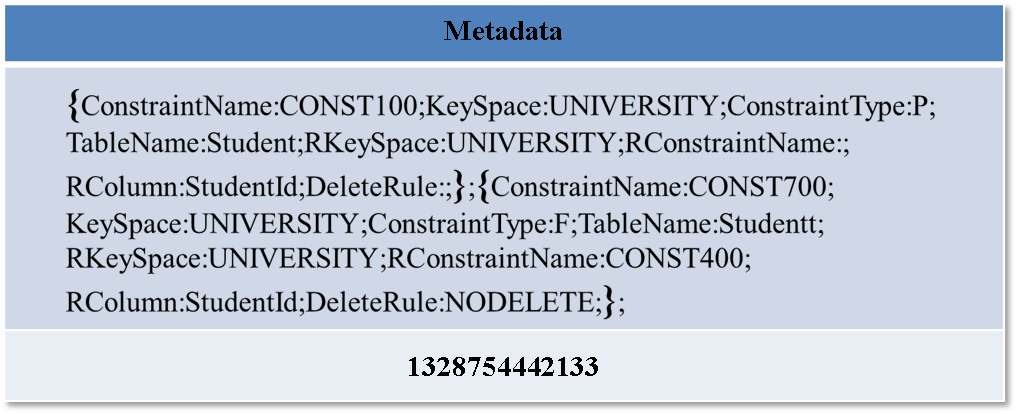
\includegraphics[width=.6\textwidth]{./figure/Solutions/Sol1-MD-Col.png}
	% 			\caption{Response Time for \texttt{insert}}\label{fr:response-insert}
			}
			\subfigure[Metadata in Supercolumns]{
				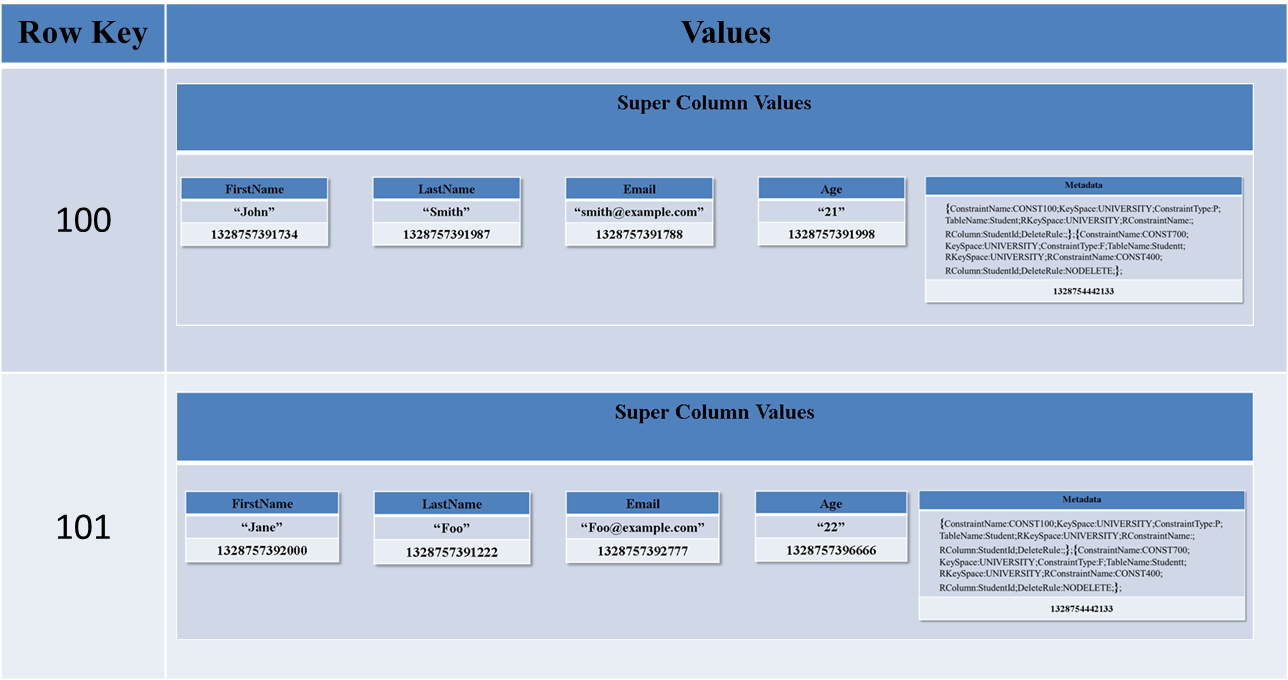
\includegraphics[width=1\textwidth]{./figure/Solutions/Sol1-MD-ColumnFamily.png}
	% 			\caption{Throughput}\label{fr:through-insert}
			} 
			\caption{Metadata storage in Solution 1}
		\end{figure}
Special characters are used within the metadata to separate the constraints and
to identify its different parts. The special characters used in this solution
are '\texttt{\{}', '\texttt{\}}','\texttt{;}' and '\texttt{:}'. The special
characters are used the following way:
	
		\begin{itemize}
			\item Each constraint is enclosed in curly brackets and separated from each
			other by the special character '\texttt{;}'. For example,in \texttt{Student}
			\texttt{CONST100} and \texttt{CONST700} are enclosed in curly braces and
			separated by '\texttt{;}'. Thus, '\texttt{\};}' marks the end of every
			constraint in the metadata.
		
		
			\item The different parts of each constraint are separated by the special character
			'\texttt{;}'. For example,  '\texttt{;}' separates the \texttt{ConstraintName}
			 and \texttt{Keyspace} and other parts in the constraints \texttt{CONST100} and
			 \texttt{CONST700}
			 
			 
			\item Each part and its value are separated by the special character
			'\texttt{:}'. For example, \texttt{ConstraintName} is separated from
			its value \texttt{CONST100} with a \texttt{:}. This helps in identifying the
			name and value for every part while parsing the metadata information
			in the \ac{API}.
			
		\end{itemize}
This metadata is extracted from each super column and processed by specific
methods within the solution so that metadata is used for validating referential
integrity. Different methods are built in the \ac{API} to support these
functionalities and described in the Implementation chapter.

In this solution, the metadata is  repeated several times within the
same column family and due to the replicated nature of the \ac{NoSQL} \acp{DBMS}
the metadata is  stored several times across the nodes in the cluster. This
increases the redundancy of the metadata and much space would be consumed
unnecessarily if the metedata is large. 

This design was inspired by the experiments done on Tokyo Cabinet, a popular
\ac{NoSQL} \ac{DBMS} by Hackl et al.  (2010), where metadata information was
stored as a part of the value in a key-value pair stored in Tokyo Cabinet. In
Hackl et al.  (2010),  metadata management is addressed in the context of huge
file systems, where metadata is stored separately in a suitable \ac{DBMS} so
that such file systems can be managed and administered efficiently without
slowing them down.  To analyse which type of \ac{DBMS} was more suitable for
such a metadata storage,  they conducted various experiments and concluded that
key-value \acp{DBMS} were more efficient in terms of speed,  memory and resource
consumption when compared to popular \acp{RDBMS}.  As a part of their
experiments, they adopted an interesting approach to store metadata in  Tokyo
Cabinet where records are stored as simple key-value
pairs in data files. Unlike Cassandra, Tokyo Cabinet does not involve data types
or columns and column families (\todo{cite}).
In their approach,  metadata about the file system used in their experiment is
inserted as a value which is associated with a unique key and the different
parts of the metadata are separated by semicolons (Hackl et al.  2010).


\section{Solution2:  Metadata as a Top Row} \label{s:design-sol2}


This solution saves the metadata embedded with the actual data and exists in the
same column family as the data. This approach is similar to Solution~1 where
metadata is stored within the same column family. But unlike Solution~1, this
solution saves the metadata only once in the column family as a top row or the
first super column in a column family with the unique \texttt{RowId}
'\texttt{-1}'. This top row has only a single column \texttt{Metadata} 
containign the metadta information and this is  unlike other super columns which
have different columns. The \texttt{Metadata} column is similar to the
Solution~1 as shown in Figure~\ref{fd:Metadata-Solution1} (a). This is possible
since Cassandra allows rows to have different number of columns, as described in Section~\ref{s::key-value-data-model}. Thus, for each entity class, the metadata
exists only once as a single row and is common for all the instances of the
entity.
In the University example  a \texttt{Student} entity has the metadata  stored as
a top row in Figure~\ref{fd:Metadata-Solution2}.
		 
	\begin{figure}[h]  
		\centering 
		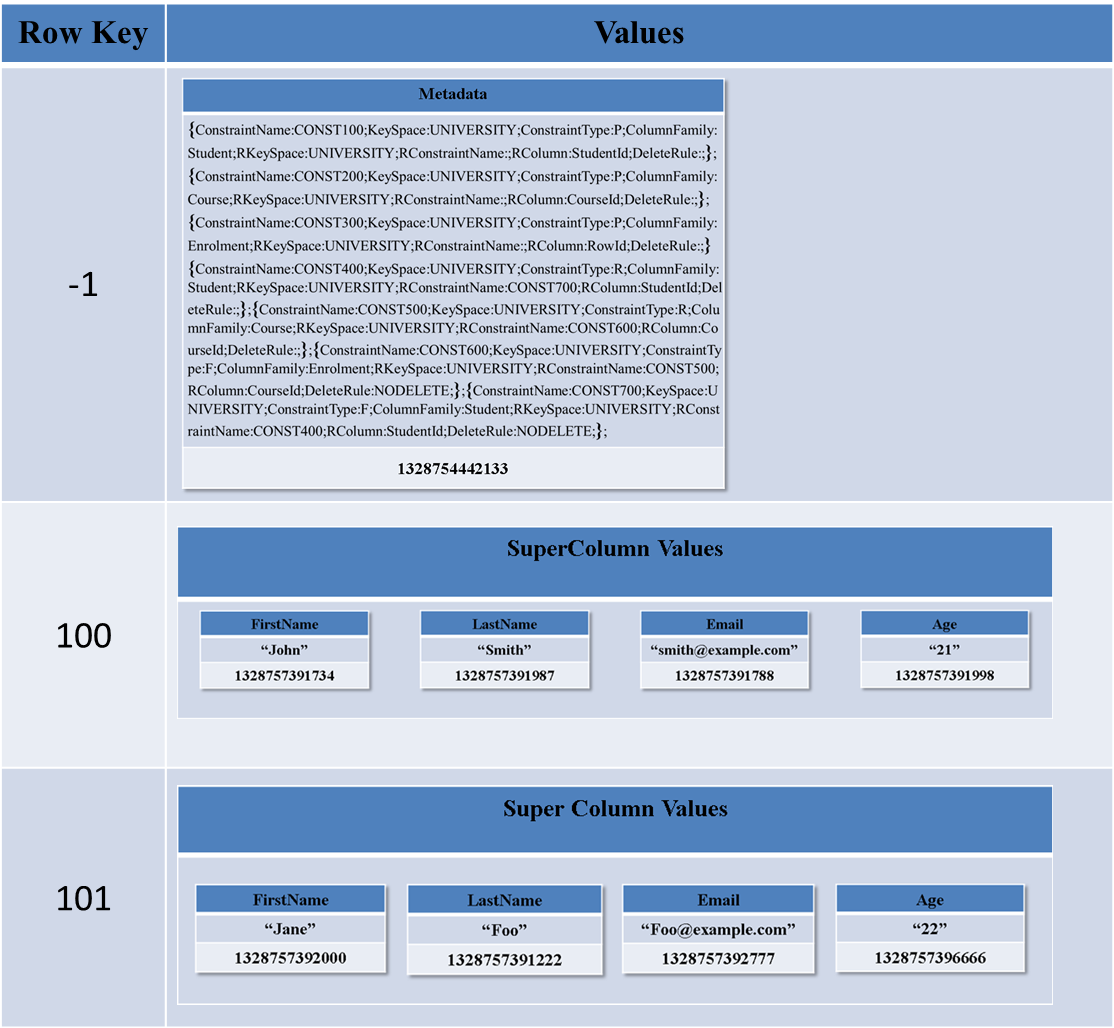
\includegraphics[width=.8\textwidth]{./figure/Solutions/Sol2-MD-ColumnFamily.png}
		\caption{Metadata storage in Solution 2}\label{fd:Metadata-Solution2}
	\end{figure}
		
The metadata in this solution contains special characters '\texttt{\{}',
'\texttt{\}}','\texttt{;}' and '\texttt{:}' to distinguish all the constraints
and its different parts and values.
The metadata stored for each column family has the following constraints:
	\begin{itemize}
	  \item  \ac{PK} constraint showing the primary key of the column family.
	  \item \ac{FK} constraints 
			\begin{itemize}
				\item In the case of a parent entity the \ac{FK} constraints are the \ac{FK}
				constraints of type '\texttt{F}' to identify the child entities when the entity
				is being updated or deleted.
				\item  In the case of a child entity the \ac{FK} constraint of type '\texttt{R}'
				would be stored along with the \ac{PK} constraint which indicates its parent
				entities.
				\item If an entity is both a parent and child entity, then its metadata would
				hold its \ac{PK} constraint, and the \ac{FK} constraints of both types.
			\end{itemize}
	\end{itemize}
	
Consider \texttt{Enrolment}  which is a child entity with parent entities
\texttt{Student} and \texttt{Course} (Figure~\ref{}). Its metadata thus contains
its \ac{PK} constraint \texttt{CONST300} and the \ac{FK} constraints
\texttt{CONST400} and \texttt{CONST500}. Since \texttt{Student} is a child
entity it  stores its \ac{PK} constraint \texttt{CONST100} and its \ac{FK}
constraint \texttt{CONST700}. Similarly, \texttt{Course} stores its \ac{PK} and
respective \ac{FK} constraints.

	\begin{figure}
	\todo{ Insert metadata top row figure for Enrolment}
	\end{figure}
% 	Thus, the metadats describes which is the
% 	primary key for the entity and the \ac{FK} constraints show which child entities dependent on the
% 	entity. The \ac{FK} constraints are particularly useful to .
	
The motivation for this solution was to overcome the redundancy of metadata
storage in Solution~1. In solution~1 metedata was stored in every super column
of a column family and replicated across the cluster along with the column
family. Solution~2 reduces this redundancy and centralises the metedata as a top
row within the column family and is common for all instances in an entity class.
This solution also ensures that when changes have to be made ot the metadata the
actual data is not accessed and only the column family of the data is accessed. 
Moreover when metadata is large, it consumes less space as it is not replicated
as widely as in Solution~1.
In other words, the aim of this design was to reduce the redundancy of metadata
in the column family whilst having metadata accessible to all the nodes by
having it embedded with the actual data.


\section{Solution3:  Metadata Column Family} \label{s:design-sol3}

This solution saves the metadata for all the entities in a separate column
family called \texttt{Metadata}.  In this approach the metadata is
decoupled from the actual data and stored in decentalised way where all the
\ac{PK} and \ac{FK} constraints for all the column famliies within the keyspace
are saved in one location. All the constraints as seen in
Figure~\ref{fd:Metadata-Constraints} are saved as super columns in the
\texttt{Metadata} column family (Figure~\ref{fd:Metadata-Solution3}). 
 
	\begin{figure}[h] 
		\centering
		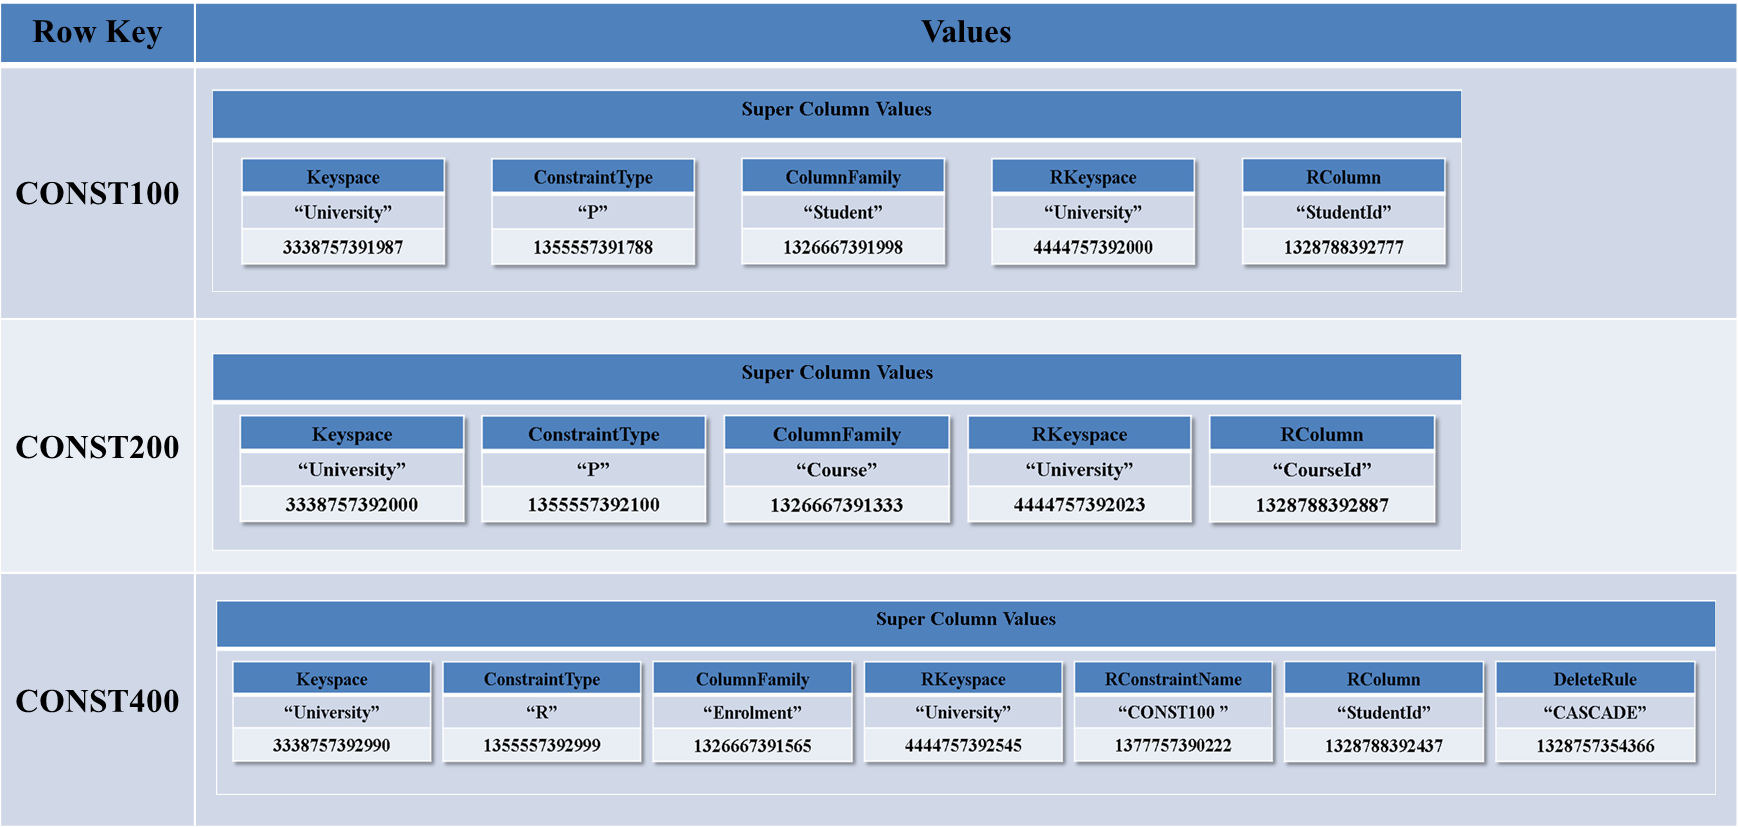
\includegraphics[width=.8\textwidth]{./figure/Solutions/Sol3-MD-ColumnFamily.png}
		\caption{Metadata Column Family in Solution 3}\label{fd:Metadata-Solution3}
	\end{figure}

The different parts of these constraints are saved as separate columns in this
approach and thus no special characters are requireed to identify the various
parts as in Solutions~1 and 2. Thus, for validating referential integruty, the
\ac{API} connects to this column family and retrieves the relevant constraints
for an entity. The different parts are accessed and its values retrived to do
the validation.

This approach is similar to the way dependency information is
stored in traditional \acp{RDBMS}, where metadata holds all the information
about entities and their dependencies and other properties. Commonly such
metadata is maintained separately from the entities in \texttt{System}tables
that can be commonly accessed by the users of the database. 

The design to decouple metadata and the actual data is inspired from the
potential problems and cases where Solutions~1 and 2 could prove to be less
useful. Such cases are when metadata undergoes frequent changes or a column
family has many constraints. When a column family has too many constraints the
value in \texttt{Metadata} column will be too large and accessing as well as
processing the large metadtaa can consume more time. In these designs, to make
changes to metadata it is required that the metadata be changed at every place
it was repeated. This meant that in Solution~1 the \texttt{Metadata} column in
every super column has to be updated every time a constraint is added, removed
or updated. In Solution~2, the top row has to be changed for all the column
famlies that have any alterations  in their constraints.
By decoupling metadtaa from the actual data it is  easier to access and retrieve
the various parts of the constraints since can be searched based on the column
names once the constraint is identified.
More importanlty it is now possible to add or remove constraints for a column
family as it is centrally stored. Any changes to metedata affects only the
\texttt{Metadata} column family and the \ac{API} does not have to access actual
data to perform these changes. 

\section{Solution4:  Metadata Cluster} \label{s:design-sol4}

Similar to Solution 3, metadata in this solution is saved in a separate column
family as shown in Figure~\ref{fd:Metadata-Solution3}. Instead of saving the
metadata as a column family within the same keyspace, it is saved in a separate
Cassandra cluster.This means that the metadata storage is decentralised and separated from the
Cassandra cluster. Metadata  is not as widely replicated as in the previous
solutions since the rpelication of metadata is only within the metadata cluster. 


% The Cassandra cluster is named ‘Test Cluster’ and consists
% of the nodes that have Cassandra with the entity column families (Student,
% Course, and Enrolment). A separate cluster called “Metadata Cluster” consists of
% nodes that have only the metadata column families.
\begin{figure}[h]
	\centering
	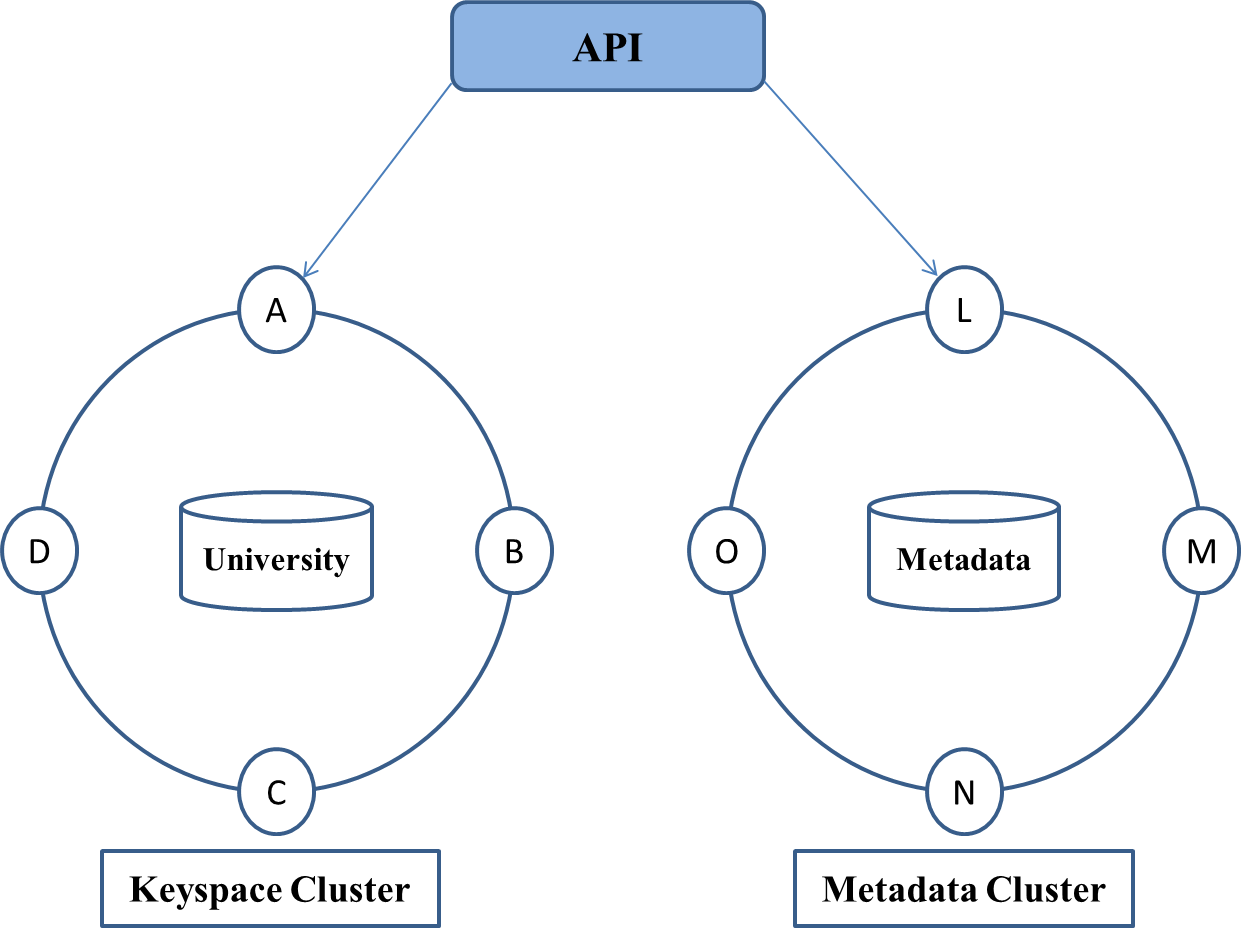
\includegraphics[width=.6\textwidth]{./figure/Solutions/Sol4-cluster-pic.png}
	\caption{Metadata Cluster in Solution
	4}\label{fd:MetadataCluster-Solution4}
	
\end{figure}

The \ac{API} connects to the Metadata cluster as well as the  cluster containing the
keyspace to perform any database operations. Whenever the metadata is
accessed the \ac{API} caches it for processing the
operations on the column famliies and to re-use the metadata. This si also
so that even if the metadata cluster is unresponsive or not active the \ac{API}
can perform operations with the cached metadata. Having metadata in a
persistence layer is effective since metedata is not frequently changed like the
actual data and also saves operational time by not having to connect to the
metadata column family each time  metadata is accessed.


% As of now, ‘Test Cluster’ is the name of the cluster for all the entity column
% families existing on Cassandra nodes. Some of the Cassandra nodes are
% Saddleback, meow, Marrakech etc. located in the ECS labs. To have a separate
% cluster of nodes for Metadata, it was required that the Cassandra configuration
% files were changed. This involved changing the listening port, RPC port, and TCP
% port to different values from that of the ‘Test Cluster’. It was also necessary
% to change the path configurations for the saved caches and log files so that it
% does not overwrite the files of the ‘Test Cluster’.
For example, in Solution 4 the metadata column family \texttt{Metadata} is
inserted into a separate cluster \texttt{MetadataCluster}, while the column
families \texttt{Student}, \texttt{course} and \texttt{Enrolment} are entered
into another cluster.

%  Just as in other solutions, metadata information needs to be checked during any
%  database operations. Every time a referential integrity check is performed, the
%  API connects to the ‘Metadata Cluster’ and retrieves the metadata information.
%  Connection pools are maintained to reuse the connections whenever needed. In
%  order to perform the database operations, the API then connects to the ‘Test
%  Cluster’ on any of its nodes. For example, if an insert operation is invoked on
%  Enrolment, it is necessary to check if the foreign keys for Student and Course
%  column families exist in their respective parent column families. The details
%  of the referenced column families are retrieved from the Metadata column family
%  in the ‘Metadata Cluster’. Once this information is processed, the API connects
%  to the referencing column families in the ‘Test Cluster’ and completes the
%  insert operation.
 Such a design approach is suitable when an application handles multiple
 keyspaces and have to store and maintain metadata for its several keyspaces. In
 these situations it is straightforward and simpler to maintain all the metadata
 in a separate cluster and decoupled form the actual data.  Even if the metadata
 cluster is unresponsive or not active the \ac{API} can perform operations with
 the cached metadata.
 
 This approach is inspired from the way most distributed systems
 save metadata in \ac{MDS} clusters (Lin Xia et al. 2009).
 For better scalability and efficient access of metadata, \ac{MDS} are
 often separate clusters in large distributed environments. In distributed
 systems such clusters  have a master \ac{MDS} and subordinate \acp{MDS}, with
 each server running on a different node. But in this solution such a management
 is not required since in a Cassandra cluster all nodes have the same
 responsibilites and do not have a master-slave configuration.
 
\section{Summary}
The significant difference in the design of all the  solutions is the way each
of the solutions store metedata. While Solution~1 stores metadata with the data
in every super column increasing the redundancy it provides easier access and to the metadata.
Solution~2 addresses reduces the redundancy of metedata and is useful when the
metadata is large for a column family since it consumes lesser space when
compared to Solution~1. Solution~3 separates the metedata from the actual data
and stores all the constraints of all the column famlies in a keyspace together
in a centralised way. This is useful when metadata has to be amended or altered.
Moreover this also removes handling the data each time metadata has to be
accessed. So the operations involving metadata need not have to process the
data. Solution~4 has a similar approach as Solution~3 but saves the metedata
column family in a separate cluster on different nodes. It also introduces
caching the metadata and thus saving oprational time and connections.

The way metadata is retrieved and
processed are different in each of the solutions since the way metadata is
stored is unique in each  solution. Referential integrity validations are
triggered when a \ac{CRUD} operation is performed on a column family. The logic
for validating the referential integrity is consistenst across all the soltuions
and specific methods exist in the \ac{API} to perform these processes. The way
the \ac{API} handles all the \ac{CRUD} operations and the validations that are
triggered during these operations and themetadata retrieval and processing
done in ecah solutions are discussed in detail in
Chapter~\ref{c:Implementation}.
% It also explains how each of the solutions retrieves and processes the metadata.

% The insert, update and delete operations are performed similar to the other
% solutions.


% These methods and all the
% solutions are incorporated  into an experimental \ac{API}, which is
% described in Chapter~\ref{c:Implementation}.

% % 
% \acresetall
% %ब
\chapter{Implementation of Referential Integrity Constraints in NoSQL DBMSs}
\label{c:Implementation}

The four solutions presented in this thesis save the foreign key relationships
between column families as metadata and each solution saves the metadata in its
own unique way.  The design of the four solutions presented in the previous
chapter was shown as an  abstract representation of the way metadata is
stored.
Such metadata is accessed whenever referential integrity
validations are triggered, that is, when \ac{CRUD} operations are invoked on
column families. The relevant  \ac{FK} constraints of a column family and
its associated \ac{PK} constraints are accessed from its metadata and processed
in order to extract the values held in the constraints. 

Since the metadata storage is different in
every solution, accessing and processing the  metadata is different in each
solution as well. 
Specific methods are designed in all the solutions to retrieve and process the
metadata, and these methods along with all the
solutions are incorporated into a single experimental \ac{API}. The
experimental \ac{API} implements the design of the solutions and provides
handlers to execute the \ac{CRUD} operations and referential
integrity validations. 
% It also implements methods to access and process metadata
% in each solution.

This chapter describes  the experimental \ac{API} and
the implementation details of the  four solutions.
Section~\ref{s:implementation-API} presents the experimental \ac{API} and
describes its most relevant components.
Section~\ref{s:implementation-MDinSolutions} describes the approaches taken by
the four solutions to retrieve and process metadata.
% Section~\ref{s:Implementation-Solution1} describes the way Solution~1 accesses and processes metadata.
% Section~\ref{s:Implementation-Solution2} describes how metadata access and
% retrieval are implemented in Solution~2.
% Section~\ref{s:Implementation-Solution3} presents how Solution~3 accesses and
% handles metadata.
% Solution~\ref{s:Implementation-Solution4} explains metadata access and
% processing techniques in Solution~4. 
Lastly, Section~\ref{s:Implementation-summary} presents a summary of the
chapter.
 

%ब
\section{Experimental API}\label{s:implementation-API}

The experimental \ac{API} was designed generically in order to ensure that it
can be used by  applications to maintain dependencies within their keyspaces
irrespective of keyspace schemas or structures of column families.  However,
applications using this \ac{API} still have to supply  the list of referential
integrity constraints as these are not automatically deduced from their
implementation. Instead, the constraints have to be introduced according to the
solution as it is explained in detail in
Section~\ref{s:implementation-MDinSolutions}.

% Thus,   this \ac{API} is made adaptable to different keyspace schemas  that
% can be deployed in column-oriented key-value \acp{DBMS}.

This \ac{API} validates the referential integrity based on the metadata provided
for the application and its column families.   It  provides the implementation of
all the four solutions as well as the required components to successfully
maintain referential integrity in Cassandra.

The  class diagram of the \ac{API} is presented  in
 Figure~\ref{f:classDiagram} alongside with the  classes that belong to 
the University keyspace example.  The design of the \ac{API} follows the
\ac{ER} model and the main components are the entities, entity managers,  and
validation handlers,  all of which are described in the next sections.
 Notice that for the sake of clarity and brevity,   the class diagram only
 contains  the relevant  methods of the classes,  favoring a simpler
explanation of the functioning of the \ac{API}. 

\begin{figure}[h]  
	\centering
	%\includegraphics[width=5cm,    height=5cm]{.  /figure/random.  jpg}
	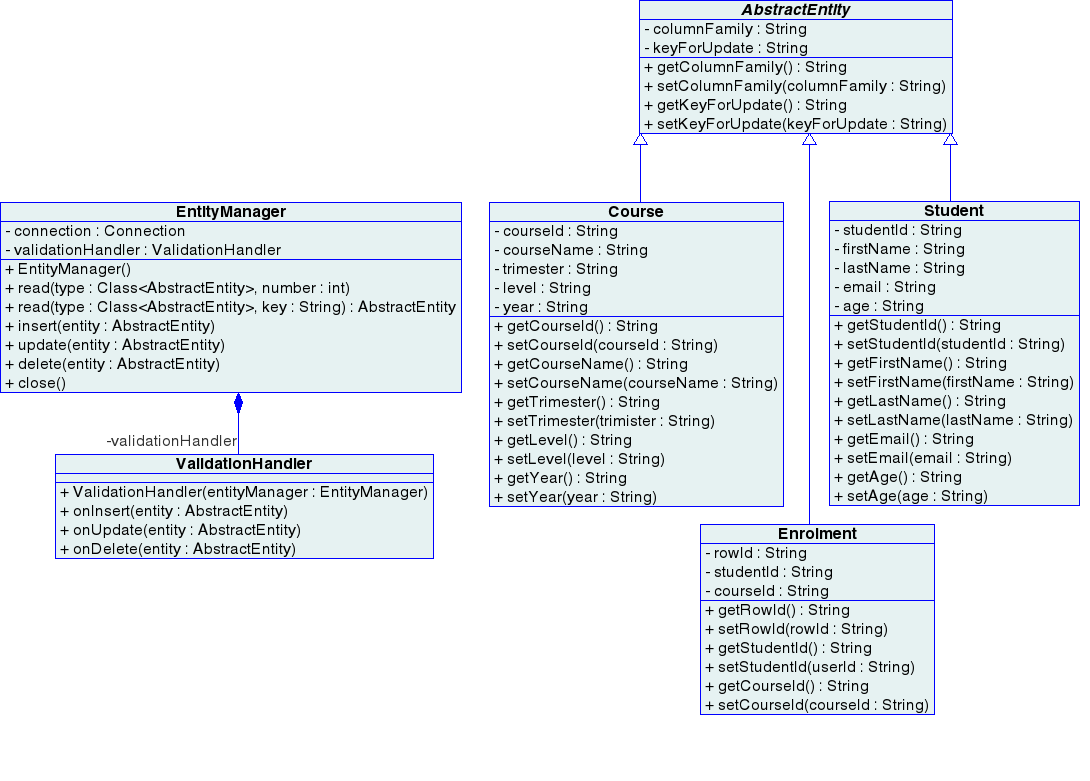
\includegraphics[width=\textwidth]{./figure/Solutions/FinalClassDiagram.png}
	\caption{Class Diagram for the \ac{API}}\label{f:classDiagram}
\end{figure}


	\subsection{Entities} 
	
	An \texttt{Entity} class contains attributes (with respective getters and
	setters) that map to columns within a specific column family.  As such,  the contents of a
	column family can be represented by a list of entity objects.  All entities in
	the \ac{API} extend from the class \texttt{Entity}  to
	aid the \ac{API} towards their management.  Particularly,  the attributes
	that \texttt{Entity} contains  are \texttt{columnFamily} which
	determines the column family to which the entity maps,  and 
	\texttt{keyForUpdate} which shall contain the new value in case the primary key
	of the entity is to be updated. 
	
	For example,   considering the University keyspace example,  \texttt{Enrolment} 
	is an entity class that  maps to the \texttt{Enrolment}  column family,  thus
	containing the attributes \texttt{RowId},  \texttt{CourseId} and
	\texttt{StudentId} which represent its respective columns.  As such,  an
	instance of \texttt{Enrolment} contains the values of one super column.  Likewise, 
	\texttt{Student} and \texttt{Course} are entity classes and their instances 
	map to   super columns in their respective column families. 
% 	For all the solutions in this \ac{API},   entities of the user applications are
% 	designed to extend the abstract class called \texttt{Entity},   which has
% 	information about the  methods for accessing and defining  entities.   For
% 	every column family,  applications derive a class from the
% 	\texttt{Entity} containing attributes. 
	Thus, the \ac{CRUD} operations that are performed on these entities  and are
	handled by the \texttt{EntityManager} class, explained next. 
		 
	\subsection{EntityManager} \label{ss:Implementation-API-EntityManager}

	The  \texttt{EntityManager} class implements  all
	the \ac{CRUD} operations to be performed on the entities.  In order to perform
	these operations,   the \texttt{EntityManager} interacts with the respective
	keyspace the entity belongs.  Moreover,  it ensures to trigger the   referential
	integrity validation process whenever a \ac{CRUD} operation requires it. The
	\texttt{EntityManager} contains an instance of \texttt{ValidationHandler} which
	ensures the validations.
	
	The \texttt{EntityManager},  before performing any operation,  requires a
	connection to the keyspace.  This connection is established using a third-party
	\ac{API} named Hector~\citep{hector}.  Hector  encapsulates the driver-level
	interface provided by Cassandra (known as Thrift) and simplifies the interaction
	with it.  Regarding the \ac{CRUD} operations,  Hector provides  a
	\texttt{Mutator} object which encapsulates the necessary procedures to perform
	such operations and to interact with the Cassandra cluster.
	 
	 Notice that  the \texttt{EntityManager} is able to generically deal with any
	 entity that derives from the \texttt{Entity} class.  It does so by using
	 reflection,  a Java  feature that is able to perform an introspection of an
	 object in runtime and retrieve its attributes and methods. 
% 	  to detect the
% 	 attributes of an object and generically invoking the getters and setters of the entities.  
	 Thus,  the  \texttt{EntityManager} is able to perform all \ac{CRUD} operations
	 on any entity by generically invoking its getter and setter methods.
	 
	 
	
% 	Hector is a high
% 	 level client that wraps the driver-level interface of Cassandra called Thrift. 
% 	 Hector  provides some features that  Thrift does not,  for example,  
% 	 fail-over mechanisms and connection pooling (\todo{cite book}).   
	 % 	 While there
% 	 are other wrappers for Thrift,  Hector was  chosen as  it is one of the
% 	 earliest wrappers and  encapsulates the interaction with the Thrift \ac{API}
% 	 and makes it simpler to access a Cassandra cluster. 	
	
	
	
	
		\subsubsection{Create}
		The \texttt{create} (or \texttt{insert}) operation stores entities in their
		respective column families. This method is provided by the
		\texttt{EntityManager} and it manages to insert these entities into their
		resective  column families which are represented by the entity class.
		For example, all the student entities are inserted into the column family
		\texttt{Student} through the \texttt{EntityManager}.  
		
		The \texttt{insert} operation triggers a referential integrity validation
		whenever a child entity is  inserted in order to ensure that its parent entities
		exist.  The validation is performed by the \texttt{onInsert} method of
		\texttt{ValidationHandler},  which is explained later.  Finally, if the
		\texttt{ValidationHandler} allows it, the \texttt{EntityManager} passes the
		entity details  including row key and column family as
		parameters to the \texttt{addInsertion} method of the Hector \texttt{Mutator}
		object.
			
		\subsubsection{Read}
		The  \texttt{read} operation retrieves  entities from the column family mapped
		by the entity class.		
		This \ac{API} provides three methods for retrieving entities: \texttt{find},
		\texttt{query} and \texttt{read}. The \texttt{find} mehtod retrieves a single
		entity given its class and the value of its primary key. The \texttt{query}
		method retrieves a list of entities given a conditional expression on a
		column  name and a column value. The \texttt{read} method retrieves a list of
		entities representing the contents of the column family.
		
		Notice that, these  operations do not prompt any referential integrity
		validation since entities are only read and their state is not changed,  unlike
		in the other operations.

		
		
		\subsubsection{Update}\label{ss:update}
		The \texttt{update} operation merges  the existing contents of an entity  with
		new contents.   In other words,  the  values of the columns an entity represents
		are updated to new values and committed into the column families.
		
		The \texttt{EntityManager} provides the following three types of updates. 
		
		\begin{description}
			\item [Case A: Update Primary Key]  where the attribute
			\texttt{keyForUpdate} is used to indicate the change in the primary key.
			Before the primary key is updated, and there are child dependencies referencing
			the primary key,  the following steps are performed to complete the
			\texttt{update} operation.
		% In order to do so,  the \texttt{EntityManager} passes the entity to the
		% \texttt{ValidationHandler}  to check for referential integrity,  retrieves the
		% list of child entities that depend on its primary key,  deletes dependencies
		% and the entity,   and update the dependencies Following this,  the steps that
		% are performed are :
\todo{FIX}
			\begin{enumerate}
			  
			  
			\item Check with the \texttt{ValidationHandler} if the entity can be updated.
		
			
			\item Set the primary key of the entity to the \texttt{keyForUpdate} value. 
			
			\item Perform an \texttt{insert} of the entity with the new primary key.
			
			\item Retrieve the list of any child entities that depend on the old primary key
			of the entity.

			\item Update the foreign keys of the list of child entities to match the value
			of the new primary key of the entity.
			
			\item Perform a \texttt{delete} operation on the old entity.
		\item

			\end{enumerate}
		
% 		In all the solutions,   an \texttt{Update} operation triggers a referential
% 		 integrity validation whenever any primary or foreign keys of any entities are
% 		updated. 
% 		The validations are performed by the \texttt{onUpdate} method of the
% 		\texttt{ValidationHandler}. 
			If the update is not a cascaded one, the child entities are not updated to
			the new primary keys. This is explained in Section~\ref{} Notice that such a
			procedure is used to circumvent the restriction of Cassandra to change a primary key.  Once a record has been
			inserted into the column family,  the primary key cannot  be changed.  This is
			known as a tombstone delete,  which prevents deleting a primary key or
			changing it. 
		
		
		
			\item [Case B: Update  Foreign Key]  where  the \texttt{ValidationHandler}
			is used to check if the foreign keys can be updated and
			the respective getter and setter methods of the entity are used to perform the
			changes. 
			
			\item [Case C: Update Attributes]  where a normal update takes place as long as
			the attributes  are not keys or referenced anywhere.
			
		\end{description}
		
		
% 		one in which ,   another in which the foriegn keys are changed
% 		and lastly the one in which attributes that are not keys or referenced anywhere
% 		are changed.  In the former case,  the attribute \texttt{keyForUpdate} is used to
% 		indicate the change in the primary key.  In the case where forieng keys are
% 		updated,   respective getter and setter methods of the  entity are used to
% 		perform the changes.  In both these cases,  referential
% 		integrity needs to be ensured. 
% 		
% % 		it uses the primary key of the entity to update it,  and the other one in which
% % 		uses the especial field \texttt{keyForUpdate} to update the primary as well as
% % 		the rest of the fields. 
% 		 
% 		When the entity to be updated does not contain a change in its keys,  a normal
% 		update takes place using its getter and setter methods.   
		
		
		\subsubsection{Delete}\label{ss:delete}
		The  \texttt{Delete} operation removes  entities from a column
		family.  As mentioned before,  due to the tombstone delete,  the primary key
		will never cease to exist,  but still the values of the columns are emptied.
		Thus, whenever empty keys are read by the \ac{API}, the entities are ignored.
		
		In all solutions,   the \texttt{Delete} operation triggers a referential
		integrity validation every time a parent entity is deleted.   This validation is
		performed by the \texttt{onDelete} method of the \texttt{ValidationHandler}, 
		which is explained in the next section.   Finally,  if the
		\texttt{ValidationHandler} allows it, the \texttt{EntityManager} passes the
		entity information to the \texttt{delete} method of Hector's \texttt{Mutator} object. 
 		
%  		Before a parent entity is deleted,  the \texttt{EntityManager} retrieves the
%  		child entities it depends upon  from he \texttt{ValidationHandler} if the
%  		 referential intergity is not violated.  The \texttt{EntityManager} deletes
%  		the child entities prior to deleting the parent entity. 
		
		\subsection{ValidationHandler}\label{ss:VH}
		The \texttt{ValidationHandler} is used by the \texttt{EntityManager} every time
		an operation triggers  referential integrity validations on any entity.
		The \texttt{ValidationHandler} has access to the \texttt{EntityManager} in order
		to look-up for dependencies and metadata of an entity as soon as  validation is
		invoked on an entity.
% The \texttt{EntityManager} passes the entity and the connection details  to
% the \texttt{ValidationHandler} to perform the validation.
		
		The \texttt{ValidationHandler} contains the  logic for checking whether an
		entity has any dependencies and verifies whether  \texttt{insert},
		\texttt{update} or \texttt{delete} operations  violate  referential integrity or
		not.   In order to ensure that these operations maintain referential integrity
		between entities,  it applies the appropriate referential integrity rules
		explained in Section~\ref{s:referential-integrity}. Similarly,  for
		\texttt{update} and \texttt{delete} operations their respective rules are
		applied.   The referential integrity validation performed by the
		\texttt{ValidationHandler} for each of these operations is discussed next.
		
	\begin{description}
	\item[onInsert:]
		In an \texttt{insert} operation,  a referential integrity validation is
		triggered before an entity is  inserted. The \texttt{ValidationHandler}  checks
		whether the entity has foreign keys and, if so, whether these refer to valid
		parent entities. That is,  it ensures that the foreign keys of the entity to
		insert match primary keys.  Otherwise, an exception is raised stating that the
		referential integrity has been violated. The following checks are performed by
		the \texttt{ValidationHandler}.
		
		\renewcommand{\labelenumii}{\arabic{enumi}. \arabic{enumii}}
		\renewcommand{\labelenumiii}{\arabic{enumi}. \arabic{enumii}. \arabic{enumiii}}
		
		\begin{enumerate}
		\item If the entity has no \ac{FK} constraints
				\begin{enumerate}
		  		\item \texttt{EntityManager} inserts the entity. 
		  		\end{enumerate}
				
		\item Else,  if the entity has \ac{FK} constraints 
		  		\begin{enumerate}
				\item Identify the parent entity class from the \ac{FK} constraint. 
				\item If foreign keys exist as  primary key in the parent entity class
				  		\begin{enumerate}
				  		\item \texttt{EntityManager} inserts the entity. 
				  		\end{enumerate}
				\item Else
				   		\begin{enumerate}
				   		  \item Raise exception. 
				   		\end{enumerate}
				\end{enumerate}   	
		\end{enumerate}
		The implementation of the \texttt{insert} operation is consistent across all the
		solutions.  
		
	\item[onUpdate:] 
		In an \texttt{update} operation,  a referential integrity validation is
		triggered before the state of an entity is changed.  The validation for an
		\texttt{update} operation is different according to whether primary keys,
		foreign keys or just regular attributes are updated.
		
		\begin{description}
		\item[Case A: Update Primary Key] When a  primary key of a
		parent entity is updated,  the \texttt{ValidationHandler} performs the
		following checks. 
		\renewcommand{\labelenumii}{\arabic{enumi}. \arabic{enumii}}
		\renewcommand{\labelenumiii}{\arabic{enumi}. \arabic{enumii}. \arabic{enumiii}}
		%\renewcommand{\labelenumiiii}{\arabic{enumi}. \arabic{enumii}. \arabic{enumiii}. \arabic{enumiiii}}
		\begin{enumerate}
		  \item If the entity has no \ac{FK} constraints 
		  	\begin{enumerate}
		  		  \item \texttt{EntityManager}  updates the entity. 
			\end{enumerate}		  	
		  \item Else if the entity has  \ac{FK} constraints  
		  		\begin{enumerate}		  	
				  \item If the \texttt{DeleteRule} for the \ac{FK} constraint is
				  \texttt{Cascade}
				    	\begin{enumerate}
				    	  \item Use \texttt{EntityManager} to
				    	   update the primary key of the entity and the foreign keys of the
				    	   child entities. 
						\end{enumerate}
				  \item Else,  if the \texttt{DeleteRule}  is
				  \texttt{NoDelete}\footnote{{Notice that \texttt{DeleteRule} is considered as the rules applied on
				  \texttt{update} operations for brevity and simplicity.}}
						\begin{enumerate}
						  \item If the entity has no child entities,  
% 						  		\begin{enumerate}
						  		   \texttt{EntityManager}  updates the entity. 
% 						  		\end{enumerate}
						  \item Else,  if the entity has child entities,  
% 						   		\begin{enumerate}
						    	  Raise exception.  
% 						    	\end{enumerate}
						\end{enumerate}
				\end{enumerate}
		 \end{enumerate}
		 
		For example,   in the University keyspace,   when a
		 \texttt{keyForUpdate} is provided for an existing  \texttt{Student}
		entity,   the \texttt{ValidationHandler}
		checks the metadata and locates the \ac{FK} constraint \texttt{CONST400} as
		seen in Figure~\ref{f:metadataInSolutions}.  Since the \texttt{DeleteRule} is
		\texttt{Cascade},  the \texttt{ValidationHandler} allows the \texttt{update}
		operation to take place as explained in Section~\ref{ss:Implementation-API-EntityManager}. 
			
% 			For example,  when the foreign key \texttt{StudentId} for one of the entities
% 		in \texttt{Enrolment} is given a new value,   then the \texttt{ValidationHandler} 
% 		identifies the parent entity class for its \ac{FK} constraint
% 		\texttt{CONST400} as \texttt{Student}.   If the new \texttt{StudentId} 
% 		exists as a primary key for any
% 		 of the  entities in \texttt{Student} entity class,   the \texttt{update} is
% 		 performed. 
		 
		\item[Case B: Update Foreign Key] When a foreign key of a child entity is
		updated,  the  \texttt{ValidationHandler} checks  the
		metadata and locates its \ac{FK} constraints.  It then follows these steps:
		\begin{enumerate}
		  \item Identify parent entity class from the \ac{FK} constraint. 
		  \item If the new foreign key exists as primary key in the parent entity
		  class
			\begin{enumerate}
				\item \texttt{EntityManager} updates  the foreign key. 
			\end{enumerate}
		  \item Else 
			\begin{enumerate}
				\item Raise exception. 
			\end{enumerate}
		\end{enumerate}
		
		\item[Case C: Update Attributes] When an attribute which is neither a primary
		key nor a foreign key is updated, the \texttt{ValidationHandler} performs no
		validations and allows the \texttt{EntityManager} to update the entity. 
		
		\end{description}
		
		The implementation of the \texttt{update} operation for these cases is
		consistent across all the solutions. 
		
	\item[onDelete:] 
		In a \texttt{delete} operation, a referential
		integrity validation is triggered before an entity is deleted.  The
		\texttt{ValidationHandler} applies the referential integrity delete rule
		and performs the following checks:
		\renewcommand{\labelenumii}{\arabic{enumi}. \arabic{enumii}}
		\renewcommand{\labelenumiii}{\arabic{enumi}. \arabic{enumii}. \arabic{enumiii}}
		
		\begin{enumerate}
% 		  \item Identify existing \ac{FK} constraints on the entity. 
		  \item If the entity has no \ac{FK} constraints 
		  		\begin{enumerate}
				  \item \texttt{EntityManager} deletes the entity. 
				\end{enumerate}
		  \item Else if the entity has \ac{FK} constraints 
				\begin{enumerate}
		  		  \item If \texttt{DeleteRule} is \texttt{Cascade}
		  		 		\begin{enumerate}
		  		 		   \item Use \texttt{EntityManager}
		  		 		   to delete the entity and its child entities. 
		  		 		\end{enumerate}
		  		  \item Else if \texttt{DeleteRule}  is \texttt{NoDelete}
						\begin{enumerate}
						  \item If no child entities exist,
% 						  		\begin{enumerate}
						  		   \texttt{EntityManager} deletes the entity. 
% 						  		\end{enumerate}
						  \item Else if child entities exist,
% 						   		\begin{enumerate}
						    		 Raise exception.  
% 						    	\end{enumerate}
						\end{enumerate}
		  		\end{enumerate}
		\end{enumerate}	
		For example,   in the University keyspace,   if a 
		\texttt{Student} entity is marked for
		deletion,  the \texttt{ValidationHandler} locates the \ac{FK} constraint 
		\texttt{CONST400} referencing \texttt{Student}. 
		Since the \texttt{DeleteRule} is \texttt{Cascade},  
		the child entities are deleted from \texttt{Enrolment} prior to deleting the
		entity from its \texttt{Student} column family.  
	\end{description}
		
%  Since metadata is stored differently in the solutions,  the operation for
% retrieving the metadata in the  \texttt{ValidationHandler} is different for
% each solution in the \ac{API}. 
% For example,   the \texttt{ValidationHandler} for Solution 1 and 2 involves
% parsing the metadata  since it is stored as a \texttt{String} along with the
% actual data while in Solution 3 and 4 it is saved as an entity class. 
	The referential integrity validation logic,  the implementation of the \ac{CRUD}
	operations and the connection settings of Cassandra  are common for
	all the solutions in the \ac{API}.  However,  the metadata access,  retrieval and
	processing are unique to each solution and handled accordingly.  The following
	sections describe how metadata is  
	accessed and processed in the \ac{API}. 
% how metadata is accessed and retrieved and the motivation for the solution's
% design. 

 
	
%ला
\section{Metadata Retrieval Approaches in Solutions}
\label{s:implementation-MDinSolutions}

In every solution,  every time referential integrity validations are triggered
by operations  performed  on  any entity,  the
\texttt{ValidationHandler} requires access to its  metadata. Even when metadata
storage is different in each solution, all of them adopt  
 one of the following two methods for retrieving and processing the
metadata. One method handles metadata as an entity and the other method handles
metadata as text. These approaches and their implementation 
are explained next.


%   metadata of the entity is
% accessed.   This thesis adopts  two fundamental approaches to implement metadata
% in solutions,  and the solutions adopt one or both of the  approaches depending
% on its metadata storage.   The two approaches process,  access and treat metadata
% in  different ways,  where one approach treats metadata as an entity with its
% own respective entity class and the other approach considers metadata as text.  
% 
% The \texttt{Entity} class and the \texttt{ValidationHandler} perform additional
% operations depending on the approach adopted in a solution.   The following
% sections describe these approaches and the way solutions implement these.  

% The referential integrity validation and the
% \ac{CRUD} operations in this solution are implemented as described in
% Section~\ref{s:implementation-API}.     
 
\subsection{Metadata as an Entity} \label{ss:implementation-MDEntityClass}
Solutions~3 and 4 store  metadata in separate column families, either in the
same cluster or in a different one, respectively.  As such, in the \ac{API}, the
metadata column family is mapped by the entity class \texttt{Metadata} which contains the
necessary information for each constraint.  These constraints are inserted 
by the \texttt{EntityManager} the same way as other entities are inserted, only
without performing referential integrity validations. Notice that the
constraints required by an application must be explicitely provided to the
\ac{API}.

 
The \texttt{Metadata} entity class stores the various parts of a constraint as
its attributes and provides their respective getter and setter methods.  Since
all the constraints in a keyspace are stored in the \texttt{Metadata} column
family, a single metadata entity refers to a single constraint. Thus, a list
of \texttt{Metadata} entities contains  all the relevant constraints for an
entity. The class diagram of the \texttt{Metadata} entity class is shown in
Figure~\ref{fi:MetadataEntityClass}.

	\begin{figure}[h] 
		\centering		
		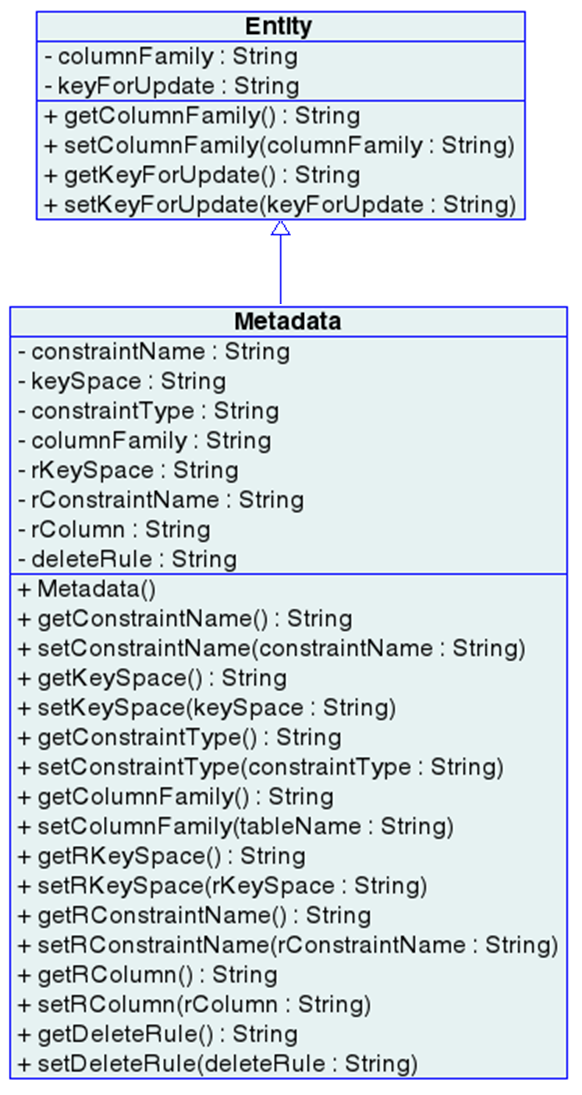
\includegraphics[width=0.4\textwidth]{./figure/Solutions/FinalMetadata.png}
		\caption{Metadata Entity Class}\label{fi:MetadataEntityClass}
	\end{figure}
	
The \texttt{ValidationHandler} retrieves the list of \texttt{Metadata} entities
relevant to the entity upon validation.  It does so by using the
\texttt{EntityManager} to read the constraints from \texttt{Metadata}.  The
\texttt{ValidationHandler} iterates through the list of 
\texttt{Metadata} entities and uses the respective getter methods in order to
retrieve the different attributes of the metadata to complete the validation. 
Notice that, in Solution~4, the list of metadata is maintained in
cache in order to re-use it for future validations of the same entity type.
Thus,  connections to the metadata cluster are avoided each time a validation
is performed.


\subsection{Metadata as Text}\label{ss:implementation-MDText}

Solutions~1 and 2 store metadata as a string of text. Solution~1 saves the
metadata within each entity in its  \texttt{Metadata} column, and
 Solution~2 saves the metadata in  the top row of the respective column
families. Notice that, Solution~2 performs an additional
 search to locate the  top row (\texttt{RowId=`-1'}) where the metadata is
 stored, and then loads it within the  entity.
 
The string of metadata within each entity contains all the constraints
 separated using special characters as explained in Section~\ref{s:design-sol1}.
These special characters serve as delimiters for the \texttt{EntityManager} to
parse and extract the information about the relevant constraints. This
information is then loaded  into the attributes of  an instance of the
\texttt{Metadata} entity class. From then on, metadata is handled as an entity
as explained in the previous section. That is, the \texttt{ValidationHandler}
uses the relevant getter methods of the \texttt{Metadata} entity class to
retrieve  the different attributes necessary to complete the validation.






% Each time an entity is loaded, the
% \texttt{EntityManager} parses its string of metadata using the special
% characters as delimiters, in order to extract each constraint and its associated
% values. 













% \section{Solution 1:  Metadata with Special
Characters}\label{s:Implementation-Solution1}

% \subsection{Metadata Storage}
% 	This solution saves the metadata embedded with the actual data and is stored in
% 	the column family belonging to the actual data. This means that metadata is
% 	included in every super column in a column family as the value of column
% 	\texttt{Metadata}. Since metadata is common for all the entities in an entity
% 	class, every super column contains the same metadata value for this column.For
% 	example, in the University keyspace, metadata in \texttt{Student} is stored in
% 	every super column as seen in Figure~\ref{f:sol1-Student-md}.
% 	
% 		\begin{figure}[H]
% 			\centering
% 			%\includegraphics[width=5cm,   height=5cm]{. /figure/random. jpg}
% 			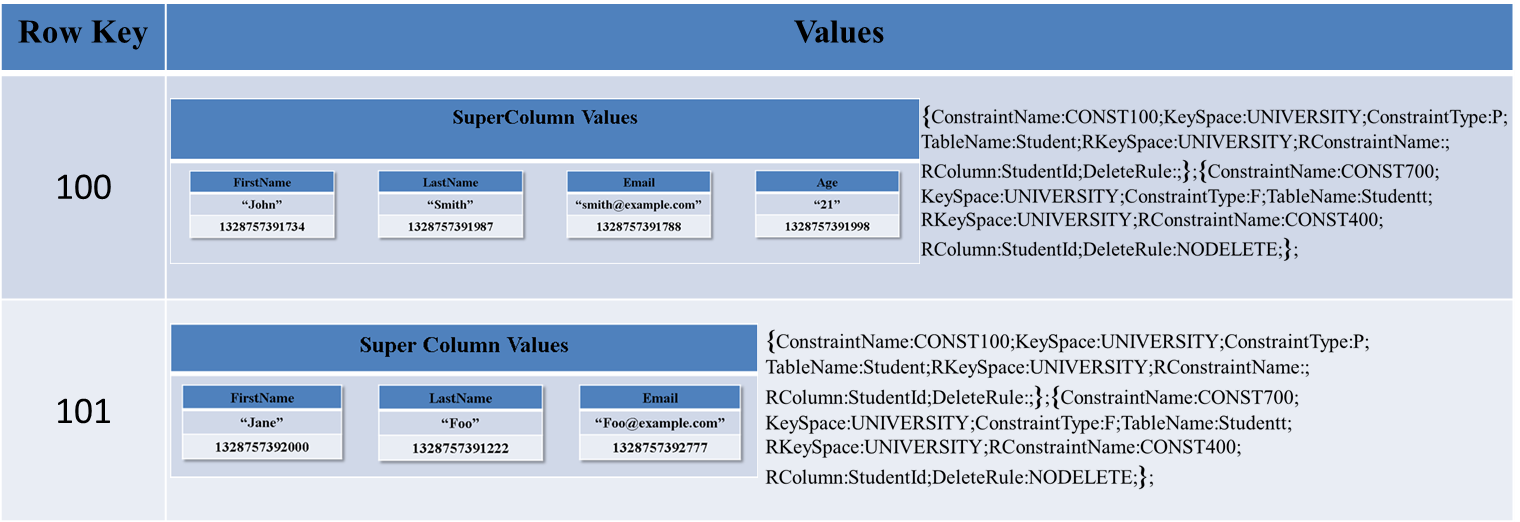
\includegraphics[width=1\textwidth]{./figure/Solutions/Solution1-Student-MD.png}
% 			\caption{Metadata storage in Solution 1}\label{f:sol1-Student-md}
% 		\end{figure}
% 		
% 	In this solution, the structure of the constraints in metadata is as described
% 	in Section~\ref{s:Metadata} and each entity class stores  its \ac{PK}
% 	constraint and related \ac{FK} constraints in the metadata. 
% 	Each entity stores the following constraints as its metadata.
% 	
% 		\begin{itemize}
% 		  \item  \ac{PK} constraint showing the primary key of the column family.
% 		  \item \ac{FK} constraints 
% 				\begin{itemize}
% 					\item In the case of a parent entity the \ac{FK} constraints are the \ac{FK}
% 					constraints of type '\texttt{F}' to identify the child entities when the entity
% 					is being updated or deleted.
% 					\item  In the case of a child entity the \ac{FK} constraint of type '\texttt{R}'
% 					is stored to indicate the parent entities.
% 					\item If an entity is both a parent and a child, then its metadata
% 					stores its \ac{PK} constraint and the \ac{FK} constraints of both types.
% 				\end{itemize}
% 		\end{itemize}
% 		
% 	For instance, \texttt{Student}  is a parent entity with a child dependendent on
% 	it, namely \texttt{Enrolment}. 
% 	Its metadata thus contains its \ac{PK} constraint \texttt{CONST100} and the
% 	\ac{FK} constraint \texttt{CONST700}. Since
% 	\texttt{Enrolment} is a child entity it  stores its \ac{PK} constraint
% 	\texttt{CONST300} and its \ac{FK} constraints \texttt{CONST400} and
% 	\texttt{CONST500}. Similarly, other entities like \texttt{Course} store its
% 	\ac{PK} and respective \ac{FK} constraints.
% 	
% 	Special characters are used within the metadata to separate the constraints and
% 	to identify its different parts. The special characters used in this solution
% 	are '\texttt{\{}', '\texttt{\}}','\texttt{;}' and '\texttt{:}'. The special
% 	characters are used the following way:
% 	
% 	\begin{itemize}
% 	\item Each constraint is enclosed in curly brackets and separated from each
% 	other by the special character '\texttt{;}'. For example,in \texttt{Student}
% 	\texttt{CONST100} and \texttt{CONST700} are enclosed in curly braces and
% 	separated by '\texttt{;}'. Thus, '\texttt{\};}' marks the end of every
% 	constraint in the metadata.
% 
% 
% 	\item The different parts of each constraint are separated by the special character
% 	'\texttt{;}'. For example,  '\texttt{;}' separates the \texttt{ConstraintName}
% 	 and \texttt{Keyspace} and other parts in the constraints \texttt{CONST100} and
% 	 \texttt{CONST700}
% 	 
% 	 
% 	\item Each part and its value are separated by the special character
% 	'\texttt{:}'. For example, \texttt{ConstraintName} is separated from
% 	its value \texttt{CONST100} with a \texttt{:}. This helps in identifying the
% 	name and value for every part while parsing the metadata information
% 	in the \ac{API}.
% 	
% 	\end{itemize}
	
\subsection{Metadata Retrieval/Extraction/Processing}
	In this solution, the metadata is read as a String by the
	\texttt{AbstractEntity} and it is parsed to extract the diffrent parts and its
	values. All the special characters used within the metadata become the
	delimiters for the String parsing and  the different parts and
	its values are converted to tokens. 
	The delimiters used for parsing are:
		\begin{itemize}
		  \item Special characters '\texttt{\{}', '\texttt{\}}' and '\texttt{;}' are
		  the delimiters for extracting each constraint from the metedata.
		  \item Special character '\texttt{;}' is the delimiter for identifying each
		  part within a constraint.
		  \item Special character '\texttt{:}' is the delimiter for extracting the
		  field name and the value from each part of the constraint.
		\end{itemize}
		
	In this solution, an enity class for metadata with the required getter and
	setter access methods is created and used to save the metadata of an entity
	whenevr any operation is invoked on it.
	The \texttt{AbstractEntity} treats metadata just like an entity and sets the
	tokenised values using the metadata entity's setter methods.
	Every time an operation is invoked on an entity the \texttt{EntityManager}
	retreves the metadata from the \texttt{Metadata} column of the entity and loads
	it as text.
		 
	 
	 
\subsection{Metadata Access}
	  
 For referential integrity validation the
	 \texttt{ValidationHandler} accesses each part of the metadata using the
	 relevant setter methods. For instance, to get information of
	the \texttt{DeleteRule} of a constraint on the entity,
	\texttt{ValidationHandler} uses the \texttt{getDeleteRule} method of the
	metadtaa entity class and likewise for all the other different parts
	of the metadata respective getter methods are used.
	 
	 The logic for the referential
	 integrity validation by the \texttt{ValidationHandler} once the String metedata is parsed is the same as described in Section~\ref{ss:VH}.

	In this solution, the metadata is saved  when entities are inserted into the
	column family and thus the metadata is a part of each of the entity.  Since the
	metadata is present as the value in every super column,  accessing the metadata
	information for referential integrity validation is as simple as accessing the
	value itself,  requiring no additional actions or connection to the
	keyspace. Saving the metadata as embedded metadata in this solution is useful
	as entities are replicated across the distributed cluster, making metadata
	easily accessible by every node in the cluster, since it is a part of the
	entity.

	The \ac{API} parses the metadata of an entity by reading any of its
	instances and need not load metadata from any external location.

	On the other hand,  the metadata for an entity would be the same for all its
	instances .  For example,  in the University example,  the metadata
	information for the \texttt{Student} entity is applicable to each of its
	instances,  indicating that each instance  should have a primary key called
	\texttt{StudentID}.
	Similarly,  all \texttt{Course} instances have the same \ac{PK} constraints
	applied on it.  When metadata is saved as a part of the  value,
	every instance of an entity will contain the constraint information
	in it's value.  Since the metadata information and constraints are same for all
	the instances of a single entity ,  this metadata is repeated every time an
	instance of the entity is inserted.  For example,  if
	\texttt{1000} \texttt{Student} instances are inserted,  the metadata for these
	\texttt{1000} instances are saved \texttt{1000} times too, along with these
	instances.  But the metadata is exactly same for all the
	instances \todo{(Figure~\ref{})}.


% 	The distributed nature of cloud \ac{NoSQL} \acp{DBMS} also means that the
% 	metadata is not only repeated several times within the same column family,  but
% 	also across the nodes in the cluster, thus increasing the redundancy of
% 	the metadata.  But such a redundancy and consumption
% 	of space to store the metadata is not a potential issue
% 	in cloud column-oriented key-value \acp{DBMS}, since storage on the cloud is
% 	inexpensive and  does not affect the economic benefits.
% 
% 	Such a storage mechanism is not expected to affect the efficiency of the
% 	cluster negatively as the metadata information is not large in size and is
% 	easily replicated along with the actual data and does not exert any extra
% 	resources in the cluster.  The performance of this solution is analysed  in
% 	Chapter~\ref{}.
% 
% 	Much research has been done in the area of  metadata management in distributed
% 	environments,  where emphasis is laid on the synchronous updates of metadata
% 	storage as well as its efficient storage and access mechanisms(\todo{cite more}
% 	Hackl et al.  2010).
% 	In Hackl et al.  (2010),  metadata management is discussed in the context of
% 	huge file systems, where metadata is stored separately in a suitable \ac{DBMS}
% 	so that such file systems can be managed and administered efficiently without
% 	slowing them down.  To analyse which type of \ac{DBMS} was more suitable for such a
% 	metadata storage,  they conducted various experiments and concluded that
% 	key-value \acp{DBMS} were more efficient in terms of speed,  memory and resource
% 	consumption when compared to popular \acp{RDBMS}.  As a part of their
% 	experiments, they adopted an interesting approach to store metadata in a
% 	key-value \ac{DBMS} ,  namely Tokyo Cabinet,  a popular \ac{NoSQL} \ac{DBMS}
% 	that stores records as simple key-value pairs in data files. Unlike Cassandra,
% 	tokyoCabinet does not involve data types or columns
% 	and so on (\todo{cite}).  In their approach,  metadata about the file system
% 	used in their experiment is inserted as a value which is associated with a unique key and the
% 	different parts of the metadata are separated by semicolons (Hackl et al.  2010).
	
% 
% \section{Solution 2:  Metadata as Top Row}\label{s:Implementation-Solution2}
	
% 	\subsection{Metadata Storage}
% 	This solution saves the metadata embedded with the actual data and exists in
% 	the same column family as the data. This approach is similar to
% 	Solution~1 where metadata is stored within the same column family. But unlike
% 	Solution~1, this solution saves the metadata only once in the column family as a
% 	top row or the first super column in a column family with the unique
% 	\texttt{RowId} '\texttt{-1}'. This top row has only a single column 
% 	\texttt{Metadata}  containign the metadta information and this is  unlike
% 	other super columns which have different columns. This is possible since
% 	Cassandra allows rows to have different number of columns, as described in
% 	Section~\ref{s::key-value-data-model}. Thus, for each entity class, the
% 	metadata exists only once as a single row and is common for all the instances
% 	of the entity.
% 	In the University example  a \texttt{Student} entity has the
% 	metadata  stored as a top row in Figure~\ref{}.
% 		 
% 	\begin{figure}
% 	\todo{ Insert metadata top row figure for Student}
% 	\end{figure}
% 		
% 	The metadata in this solution contains
% 	special characters '\texttt{\{}', '\texttt{\}}','\texttt{;}' and '\texttt{:}'
% 	to distinguish all the constraints and its different parts and values.
% 	The metadata stored for each column family has the following
% 	constraints:
% 	\begin{itemize}
% 	  \item  \ac{PK} constraint showing the primary key of the column family.
% 	  \item \ac{FK} constraints 
% 			\begin{itemize}
% 				\item In the case of a parent entity the \ac{FK} constraints are the \ac{FK}
% 				constraints of type '\texttt{F}' to identify the child entities when the entity
% 				is being updated or deleted.
% 				\item  In the case of a child entity the \ac{FK} constraint of type '\texttt{R}'
% 				would be stored along with the \ac{PK} constraint which indicates its parent
% 				entities.
% 				\item If an entity is both a parent and child entity, then its metadata would
% 				hold its \ac{PK} constraint, and the \ac{FK} constraints of both types.
% 			\end{itemize}
% 	\end{itemize}
% 	
% 	Consider \texttt{Enrolment}  which is a child entity with parent entities
% 	\texttt{Student} and \texttt{Course} (Figure~\ref{}). Its metadata thus
% 	contains its \ac{PK} constraint \texttt{CONST300} and the \ac{FK} constraints
% 	\texttt{CONST400} and \texttt{CONST500}. Since \texttt{Student} is a child
% 	entity it  stores its \ac{PK} constraint \texttt{CONST100} and its \ac{FK}
% 	constraint \texttt{CONST700}. Similarly, \texttt{Course} stores its \ac{PK} and
% 	respective \ac{FK} constraints.
% 
% 	\begin{figure}
% 	\todo{ Insert metadata top row figure for Enrolment}
% 	\end{figure}
% 	Thus, the metadats describes which is the
% 	primary key for the entity and the \ac{FK} constraints show which child entities dependent on the
% 	entity. The \ac{FK} constraints are particularly useful to .
	
	\subsection{Metadata Retrieval}
	Since the metadata holds all the constraints and its various parts, the
	\ac{API} needs to extract each constraint and its different parts to validate
	referetntial integrity for an entity. For this it performs \texttt{String}
	parsing as described in Section~\ref{s:sol1-real} since metedata is read as a
	\texttt{String} while it is retrieved.
	
	In this solution, an enity class
	for metadata with the required getter and setter access methods is created and
	used to save the metadata of an entity whenevr any operation is invoked on it.
	For every operation on an entity the \texttt{AbstractEntity}
	reads its metadata from the top row of the entity class as a \texttt{String}
	and each part of the metadata is tokenised to column names and its values.
	The \texttt{AbstractEntity} treats metadata just like an
	entity and sets the tokenised values using the metadata entity's setter
	methods.
	The parsing of the metadata and its conversion to an entity using the access methods is the same as
	in Solution~1. The special characters become the delimiters for parsing the
	metadata just like in Solution~1
	
	\subsection{Metadata Access}
	The metadata is accessed by the \texttt{ValidationHandler} to
	validate referential integrity for entities. Since the metedata for each entity is
	parsed and converted ot an entity by the \texttt{AbstractEnityt}, 
	the \texttt{ValidationHandler} uses the appropriate getter methods to retrieve
	each part of the metedata. For instance, to get information of
	the \texttt{DeleteRule} of a constraint on the entity,
	\texttt{ValidationHandler} uses the \texttt{getDeleteRule} method of the
	metadtaa entity class and likewise for all the other different parts
	of the metadata respective getter methods are used.
	
% 	\subsection{Motivation for the approach}
% 	The motivation for this solution was to overcome the redundancy of metadata
% 	storage in Solution~1. In solution~1 metedata was stored in every super column
% 	of a column family and replicated across the cluster along with the column
% 	family. Solution~2 reduces this redundancy and centralises the
% 	metedata as a top row within the column family and is common for
% 	all instances in an entity class. This solution also ensures that when changes have to be made ot
% 	the metadata the actual data is not accessed and only the column family of the
% 	data is accessed.  Moreover when metadata is large, it
% 	consumes less space as it is not replicated as widely as in Solution~1. 
% 	In other words, the aim of this design was to reduce the redundancy of metadata
% 	in the column family whilst having metadata accessible to all the nodes by
% 	having it embedded with the actual data.
% 	This involves using a lot of disk space for storing the
% 	metadata, especially considering the number of times an entity class is
% 	replicated over a cluster of nodes. When the number of entity classes and
% 	\ac{FK} constraints between them are large, the size of the metadata also
% 	increases. Such large metadata will involve more parsing operations and when
% 	the metadata is repeated in every super column and widely replicated it is
% 	redundant use of storage space.

% 
% %ब
\section{Solution 3:  Metadata Column Family}\label{s:Implementation-Solution3}

In Solution~3, metadata is saved in a separate column family called
\texttt{Metadata}within the cluster, which contains all the constraints within a
keyspace. To validate referential integrity, the appropriate constraints of an
entity have to be retrieved and accessed from \texttt{Metadata} by the handlers
in the experimental \ac{API}. The way metadata is retrieved, deciphered and accessed
are discussed in the following sections.
 
\subsection{Metadata Retrieval}
In this solution, constraints are inserted into \texttt{Metadata} column family
in the same way as entities are inserted into their respective entity
classes. 
% For example, students are inserted into \texttt{Student} entity
% class. 
Here, constraints are treated as entities of \texttt{Metadata} entity
class. Note that users of the experimental \ac{API} have to provide the
constraints of the entire keyspace to insert them into \texttt{Metadata}. Moreover, 
 constraints are inserted into \texttt{Metadata} using the \texttt{insert}
operation and this operation is designed to prevent referential
integrity validations for metadata entities.

In this solution, \texttt{Metadata} is considered as an entity class and has the
necessary setter and getter access methods for its attributes. The attributes
for this entity class are the different parts of a constraint. The
\texttt{Metadata} entity class is the same as shown in
Figure~\ref{fi:MetadataEntityClass}. Unlike Solutions~1 and 2, Solution~3
performs no additional operations like String parsing  to
retrieve constraint information from the metadata.

\subsection{Metadata Access}

% To ensure referential integrity, the \texttt{ValidationHandler} accesses the
% relevant constraints of an entity.


For the \texttt{ValidationHandler} to perform validations, it is essential that
it accesses only the relevant constraints of an entity from all the constraints
stored in the \texttt{Metadata} entity class. To distinguish the relevant
constraints of an entity, the \texttt{ValidationHandler} iterates through the
constraints of \texttt{Metadata} and identifies the constraint that have the
entity as the value for its \texttt{ColumnFamily}.
Consider Figure~\ref{fd:Metadata-Solution3} which shows a few constraints in
\texttt{Metadata}. To locate the constraints of \texttt{Student} entity class,
the constraints with \texttt{ColumnFamily} containing the value
\texttt{Student} have to be identified, which in this example is constraint
\texttt{CONST100}.
Thus, the relevant \ac{PK} and \ac{FK} constraints of an entity are identified
by the \texttt{ValidationHandler}.

 Once the relevant constraints are
accessed,  the\texttt{ValidationHandler} performs
the necessary validations by accessing the values from the relevant
constraints using \texttt{Metadata} getter methods, similar to Solutions~1 and
2.


 
% 
% %ब
\section{Solution 4:  Metadata Cluster}\label{s:Implementation-Solution4}
In Solution~4, metadata is saved in a separate column family called
\texttt{Metadata} similar to Solution~3, but it is stored and maintained in a
separate cluster. Figure~\ref{fd:MetadataCluster-Solution4} illustrates the
separate clusters used in this solution. To access the metadata of an entity for 
performing validations, the
metadata cluster has to be accessed primarily. The approach to retrieve, process
and access metadata are discussed in the sections below.

\subsection{Metadata Retrieval}
The constraints are treated as entities and inserted into the \texttt{Metadata}
entity class as in Solution~3. Like Solution~3, the constraints
are provided by the users and inserted using the \texttt{insert} operation which
is designed to prevent referential integrity validations for metadata entities.
 To insert constraints into \texttt{Metadata}, a separate
connection is established to the \texttt{MetadataCluster} and to insert the other entities
into their respective entity classes in the keyspace another connection is
maintained to the \texttt{KeyspaceCluster}.

The constraints are retrieved from  \texttt{Metadata}, which 
maintained in the \texttt{MetadataCluster}, using the connection object
established for connecting to this cluster.  \texttt{Metadata}
has the necessary getter and setter methods to access its attributes which are
the different parts of a constraint. Additional operations like string parsing
are not required in this solution although a separate connection is required.

\subsection{Metadata Access}

 
Whenever an operation is invoked on an entity, the \texttt{ValidationHandler}
accesses \texttt{Metadata} and the relevant constraints of the entity are
extracted from \texttt{Metadata} by identifying constraints that have  the entity as the value
for its \texttt{ColumnFamily} field, which is similar to Solution~3.The relevant constraints
are stored as a list and maintained as cache till the operation is completed.
Hence, all the relevant \ac{PK} and \ac{FK} constraints for an entity class are
stored in the cache and reused for future operations on the entities of that
type.% 
% stored as cache by . For all the operations on entities of the entity class, the
% cached metadata is used. A connection is established to the metadata cluster in
% order to access the \texttt{Metadata} column family.  
The \texttt{ValidationHandler} accesses the values form the relevant constraints
using the getter methods of the \texttt{Metadata} and validates referential
integrity for entities.

% In this solution, the relevant constraints of an
% entity are accessed from the \texttt{Metadata} entity class using its getter
%  methods, similar to the previous solutions.  

\section{Summary}\label{s:Implementation-summary}

This chapter presented the implementation details of the experimental \ac{API}
and the way the solutions retrieve and process metadata. The experimental
\ac{API} is composed of a class \texttt{Entity} which maps to columns in the
column families, a class \texttt{EntityManager} which  performs all the
\ac{CRUD} operations on the entities, and a class \texttt{ValidationHandler}
which is in charge of checking and ensuring that referential integrity is
maintained in the keyspace at all times. These classes, while providing the fundamental
operations on generic entities, can also be derived to suit custom
application requirements. 

In order for the \texttt{ValidationHandler} to ensure referential integrity, it
must retrieve the metadata associated to the entity upon validation.  Even when
solutions store the metadata in different ways, retrieving and processing it comes down to  either using a string of text or
using a \texttt{Metadata} entity.
Solution~1 and~2 store the  metadata as text, the former  within the
entities while the latter in the top row of the column family. Hence,
both solutions require the \texttt{EntityManager} to
first parse and extract the necessary information of the constraints, and then .
load these constraints into a list of \texttt{Metadata} entities in order to
simplify its handling.
  Solution~3 and~4 store the metadata in column families, the former within the
  same cluster while the latter uses a dedicated metadata cluster. Since
  metadata has its own column family, each constraint is naturally mapped into
  a \texttt{Metadata} entity. Thus, metadata can be   retrieved by using
  the \texttt{EntityManager} and handling the \texttt{Metadata} as any other
  entity. 

The next chapter presents the experimental design used to evaluate  the
performance of each solution implemented within the \ac{API}.



% parsing of the metadata to extract the constraint values and uses the getter methods of the
% \texttt{Metadata} entity class  to access these values.
% Similarly, Solution~2 also saves metadata as text , but executes an
% additional operation to search and identify the top row in a column family.
% Solution~3 saves metadata as an entity and requires no
% additional operations to process metadata, but has to iterate through the
% \texttt{Metadata} column family to identify the relevant constraints of an
% entity.
% Likewise, Solution~4 saves metadata as an entity and performs a search to
% retrieve the relevant constraints from \texttt{Metadata}, but caches the
% metadata to avoid connecting to the metadata cluster in every operation.

% Similarities exist in solutions that have similar approaches of metadata
% storage. Some of the approaches to extract metadata and 
% Solutions~1 and 2 adopt similar approaches of implementing metadata and they
% have similar metadata retrieval approaches where  these solutions use special characters and
% perform String parsing and treats metadata as an entity class. Solutions~3 and 4
% have a similar metadata storage where metadata is stored away from the actual
% data. Hence their metadata retrieval and access are similar except for the
% additional connection and metadata cache in Solution~4.

% Although approaches to implement metadata are similar in some solutions, every
% solution has a different metadata storage and thus 
% perform some adadopts
% different approaches to extract and process metadata and 
% perform differently when its implementation is evaluated. 

% For example, Solution~2 includes an additional search withint the colum
% family, Solution~3 requires a scan of the \texttt{Metadata} column family to
% locate the ocorrect constraints and Solution~4 requires an additional
% connection.
% The parsing of the metadata and its conversion to an entity using the access
% methods is consistent in Solutions~1 and 2 while. The special characters
% become the delimiters for parsing the metadata just like in Solution~1


%  % As mentioned previously,  cloud column-oriented key-value \acp{DBMS} lack %
% referential integrity constraints to maintain foreign key relationships,  as %
% seen in traditional \acp{RDBMS},  due to its non-relational data model.
% % Moreover,  these cloud \acp{DBMS} do not normalise data nor maintain %
% relationships.
% Traditionally, referential integrity constraints are imposed on data items of
% a database to maintain foreign key relationships. These relationships are
% maintained by correctly identifying and preserving the data dependencies
% existing between the data items.
% % Traditionally, foreign key relationships are % maintained by correctly
% identifying and preserving the data dependencies existing between data items
% in a database.
% % These dependencies are maintained and  validated by imposing referential %
% integrity constraints on data items.
% Most popular traditional \acp{RDBMS} preserve such dependency information in
% their \texttt{System} tables or data dictionaries.  These tables store the
% necessary information  which is required to maintain valid dependencies. The
% information stored in such tables include table names,  primary and foreign
% keys among others.
% This can be seen in popular \acp{RDBMS} like  MS SQL Server,  PostgreSQL,
% Oracle, and so on.
%  For example,  in MS SQL Server 2000, \texttt{sysforeignkeys} is a
% \texttt{System} table which stores the information of all foreign keys of
% every table in a database, and \texttt{sysreferences} stores the mappings of 
% foreign keys to the referenced primary key columns (\todo{\citep{sys:msdn}}).
% Information in these \texttt{System} tables consist of  the names of tables
% and its constraints,  unique identifiers of referenced and referencing
% columns,  among others.
% In PostgreSQL, such information is saved as views which contain the dependency
% information of data items in a database.
% The view \texttt{table\_constraints} contains the information for all the
% constraints in every table owned by the current user. (\todo{\cite{}}).
% Similarly, Oracle uses a \texttt{SYSTEM} meta-database to hold such constraint
% information.
% In general, \texttt{System} tables or views with information about the
% existing dependencies  are looked up by these \acp{RDBMS} whenever referential
% integrity checks are triggered \citep{sys:msdn}.
%   The solutions presented in this chapter save the dependency information as
% metadata. This metadata contains relevant  information about  foreign key
% relationships in keyspaces and primary keys of column families. It is accessed
% whenever an operation is performed on the data and referential integrity needs
% to be validated.
%   This chapter describes  four  solutions  that implement referential
% integrity constraints in a cloud \ac{NoSQL} \ac{DBMS}.
% Section~\ref{s:Metadata} describes the metadata used by the solutions to store
% the dependency information.
% Section~\ref{s:API} describes the design and implementation of the
% experimental API developed to integrate all the four solutions.
% Section~\ref{s:sol1} describes  the first solution, which implements
% referential integrity constraints by saving metadata along with the actual
% data.
% Section~\ref{s:sol2} describes the second  solution where metadata is saved as
% a top row. Section~\ref{s:sol3} describes the third solution which saves
% metadata separate from the actual data.
% Section~\ref{s:sol4}  describes the fourth solution which saves metadata in a
% separate cluster.
% Finally, Section~\ref{s:solutions-summary} presents a brief summary of this
% chapter.
%  \section{Metadata}\label{s:Metadata} Metadata in \acp{DBMS} provide
% information about the data stored within the databases.
% It may contain details related to schemas, constraints,  primary and foreign
% keys, and so on.   As previously mentioned,  most traditional \acp{RDBMS}
% maintain such metadata within their \texttt{System}  tables or data
% dictionaries.
% In Apache Cassandra, the \ac{DBMS} of interest, metadata is stored in a
% keyspace named \texttt{System} and it contains information about the cluster
% and its nodes along with information related to the keyspaces, column
% families, and so on (\todo{cite BOOK}).
% Even when Cassandra has a  \texttt{System} keyspace to store metadata, it is
% read-only and hence it cannot be modified to store additional metadata about
% referential integrity constraints.
% %  As % previously mentioned ,  most traditional \acp{RDBMS} % maintain such
% metadata within their \texttt{System} tables or data dictionaries.
% % Such metadata is decoupled from the actual data and its operations,  so that
% % retrieving the metadata is faster since it does not involve handling the
% actual % data(\todo{cite Duval}).
% % It has been studied that the \ac{DaaS} is moving towards maintaining
% metadata in % the cloud \acp{DBMS},  where commonly this metadata stores
% information about the % nodes in a distributed cluster (\todo{cite
% Bin(2010)}).  For  maintaining the % scalability required in such cloud
% \acp{DBMS}, metadata is often decoupled from % the actual data so that
% accessing metadata does not cause a bottleneck in % performance.  Cassandra
% maintains  metadata about the nodes in a % cluster  in a separate keyspace
% named \texttt{System}, which stores the % properties of every node, for
% example the node tokens,  the name of the % cluster to which  nodes belongs
% to, information about the stored keyspaces and % column families and so
% on(\todo{cite BOOK}).
% % As per the design of Cassandra,  the \texttt{System} keyspace cannot be
% modified % and thus  the metadata for the   solutions cannot be incorporated
% in this % \texttt{System} keyspace.  Hence,  for preserving the metadata in
% each % solution implements a  different strategy In other words, metadata is
% associated % with actual data in different ways.  Associations can be
% classified as % (\todo{cite Duval}):
% Hence,  for preserving the metadata, each solution implements a  different
% strategy in which metadata is associated with actual data. Solutions~1 and~2
% use embedded metadata, that is, metadata is created with the actual data
% (\todo{cite Duval2009}); while solutions~3 and~4 associate metadata separately
% from the actual data.  Notice that, the structure of the metadata is kept the
% same across all the solutions even when  the way of storing and associating
% this metadata is different in each.
%  The role of metadata in  the solutions is primarily to hold the necessary
% information required to maintain referential integrity. The metadata contains
% information about primary keys,   foreign keys,  referenced and referencing
% column family details, constraints, and others.  The constraints considered in
% the solutions can be either \ac{PK} or \ac{FK} constraints. \ac{PK}
% constraints specify which column is the primary key of a column family, while
% \ac{FK} constraints (or referential integrity constraints) determine the
% foreign key relationship between two column families, that is, the column of a
% column family which  is dependent on the primary key  column of another column
% family.  Hence, for each column family with a primary key,  the metadata 
% contains one \ac{PK} constraint  and  as many \ac{FK} constraints as foreign
% key relationships.
% % Notice that, throughout %  the solutions, the structure of metadata
% containing these constraints is % consistent despite.
%  The structure of the metadata is shown in Figure~\ref{f:metadataInSolutions}.
%  This structure contains information about a University keyspace example in
% which  a simple schema is applied for the keyspace. In this example,  the
% details of the students are saved in  the \texttt{Student} column family and
% the course details in the \texttt{Course} column family.
% The enrolment details of students are saved in the \texttt{Enrolment} column
% family by associating students to courses and hence having foreign key
% relationships to both \texttt{Student} and \texttt{Course} column families.
% All the column families have unique primary keys and their \ac{PK} constraints
% are saved in the metadata as presented in Figure~\ref{f:metadataInSolutions},
% while the foreign key relationships between \texttt{Enrolment},
% \texttt{Student} and \texttt{Course} are saved as \ac{FK} constraints.  For
% instance, consider in Figure~\ref{f:metadataInSolutions} the \ac{PK}
% constraint \texttt{CONST100}, for the \texttt{Student} column family, and the
% \ac{FK} constraint \texttt{CONST400} for the foreign key relationship between
% \texttt{Enrolment} and \texttt{Student}.
%  \begin{figure}[h] \centering 
% \newcolumntype{C}{@{\hspace{2.5pt}}>{\scriptsize}c@{\hspace{2.5pt}}}
% \begin{tabular}{CCC CCC CC} \toprule \bfseries ConstraintName & \bfseries
% Keyspace & \bfseries ConstraintType & \bfseries ColumnFamily & \bfseries
% RKeyspace & \bfseries RConstraintName & \bfseries RColumn & \bfseries
% DeleteRule\\
% \midrule CONST100 & University & P & Student & University & & StudentId &\\
% \rc CONST200 & University & P & Course & University & & CourseId &\\
% CONST300 & University & P & Enrolment & University & & RowId &\\
% %   \hline %   \hline \rc CONST400 & University & R & Enrolment & University &
% CONST100 & StudentId & CASCADE\\
% CONST500 & University & R & Enrolment & University & CONST200 & CourseId &
% NODELETE\\
% \rc CONST600 & University & F & Course & University & CONST500 & CourseId &
% NODELETE\\
% CONST700 & University & F & Student & University & CONST400 & StudentId &
% CASCADE\\
% \bottomrule \end{tabular} \caption{Metadata for the
% Solutions}\label{f:metadataInSolutions} \end{figure}   Specifically, the
% structure of the metadata contains:
%  \begin{itemize}  \item \texttt{ConstraintName:} is the name assigned for
% every constraint and it uniquely identifies an existing \ac{PK} or \ac{FK}
% constraint in the metadata.
% For example,  \texttt{CONST100} and \texttt{CONST400} are the
% \texttt{ConstraintNames}.
%  \item \texttt{Keyspace:}represents the name of the Keyspace the constraint
% belongs to.
%  \item \texttt{ConstraintType:} denotes the type of the constraint and the
% possible values are '\texttt{P}', '\texttt{R}' and '\texttt{F}'.
% %   The former referes to  a \ac{PK} constraint while the latter represents  a
% %    \ac{FK} constraint.
% A \ac{PK} constraint is referred by '\texttt{P}' while '\texttt{R}' and
% '\texttt{F}' are two representations of \ac{FK} constraints.
% '\texttt{R}' represents the Referential Integrity Constraint (or the \ac{FK}
% constraint) a child entity has on a parent primary key and '\texttt{F}' shows
% the  existing dependencies on a parent entity.
% For example, \texttt{CONST400} shows that the the parent entity for
% \texttt{Enrolment} is \texttt{Student}. \texttt{CONST700} shows that parent
% entity \texttt{Student} has child dependencies on it. Notice that, the
% constraint type '\texttt{F}' is primarily used to locate the child
% dependencies for a parent when it is deleted or updated.
% %  \begin{itemize} %    \item  '\texttt{P}' represents a \ac{PK} constraint % 
%   \item '\texttt{R}' represents a   \item \texttt{ColumnFamily:} refers to the
% column family this constraint exists in. For example,  the \ac{PK} constraint
% \texttt{CONST100}  exists in column family \texttt{Student} and the column
% family of the \ac{FK} constraint \texttt{CONST400} is \texttt{Enrolment}.
%  \item \texttt{RKeyspace:}is the name of the keyspace on which this constraint
% is applied.  In the example, constraints  are applied in  the keyspace
% \texttt{University}.
%  %   In other words, it indicates which primary key %   is referenced or which
%.
% \item \texttt{RConstraintName:} For \ac{FK} constraints,
% \texttt{RConstraintName} represents the constraint that is referenced. For
% constraint type '\texttt{R}' this represents the referenced \ac{PK} constraint
% and for constraint type '\texttt{F}' it shows  the child dependencies for a
% parent entity. In the example, the \ac{FK} constraint \texttt{CONST400}
% references the \ac{PK} constraint \texttt{CONST100},  which means that
% \texttt{Enrolment} has a foreign key relationship with \texttt{Student}.
% In \texttt{CONST700} this field indicates that \ac{FK} constraint
% \texttt{CONST400} exists for \texttt{Student}. Notice that in a \ac{PK}
% constraint this field is left blank since it has no references to other keys.
%  \item \texttt{RColumn:}  indicates the primary key column on which this
% constraint is applicable.  For \ac{PK} constraints,  this holds the name of
% the primary key column. For \ac{FK} constraints, this field denotes the
% referenced column.  This example shows that the \ac{PK} constraint
% \texttt{CONST100} is applied on the primary key column \texttt{StudentId} of
% \texttt{Student} column family. The \ac{FK} constraint \texttt{CONST400}
% shows that the referenced column is \texttt{StudentId},  indicating that
% \texttt{Enrolment} references  primary key column \texttt{StudentId} of
% \texttt{Student}.
%  \item \texttt{DeleteRule:}stores the type of data manipulation rule
% applicable on this constraint. The possible values are  \texttt{Cascade} and
% \texttt{NoDelete}.  This field is not applicable  for \ac{PK} constraints
% since data manipulation rules are associated with constraints that hold
% dependency information like the \ac{FK} constraints.
%  \end{itemize}  Metadata in the solutions are accessed whenever referential
% integrity validations are triggered to extract information about \ac{FK}
% constraints.
% Specific methods are designed in all the solutions to retrieve and process the
% metadata in order to validate referential integrity.  These methods and all
% the solutions are incorporated  into an experimental \ac{API}, which is
% described in the following section.



%  \section{Limitations}\label{s:lim}
% Transaction
% cascade on one level of nesting
% unique or composite keys
% school network  -->  experimental design




b
% % 
% % 
% \acresetall
% %ब
\chapter{Experimental Design}

\todo{Check number of enrolments, introduce all metadata, and retrieve 
details of cassandra cluster from my computer}

The implementation of the four solutions  introduces referential integrity
constraints and validations in Cassandra, which are 
not provided by this \ac{DBMS} at the moment of writing. In order to evaluate
 the performance of these four solutions, experiments are 
  conducted by using the implemented \ac{API} described in
  Section~\todo{Section}.   The goal of the experiments is to determine how
  each solution affects the performance of  Cassandra in \ac{CRUD}
  operations, especifically in those where referential integrity validations are
  triggered (namely Create, Update and Delete).

The experimentation is performed on the example application presented across
chapters: the University keyspace. In such an application, different constraints
are added and allow to test the performance under such different application
requirements. The performance of the  solutions provided for ensuring
referential integrity  is measured based on response time and throughput.

This chapter is structured as follows.
Section~\ref{sexp:BenchmarkKeyspace} describes the example application 
used for the experiments. Section~\ref{sexp:CassandraCluster} provides the
details of the nodes used in the Cassandra cluster. Section~\ref{sexp:ExperimentalSetup}
describes the experimental setup to evaluate the performance of the solutions.
Section~\ref{sexp:PerformanceIndicators} presents the performance indicators
 considered for measuring the results from the experiments. Finally,
Section~\ref{sexp:Summary} presents a summary of the chapter.


\section{Example application} \label{sexp:BenchmarkKeyspace}
% In order to asses the performance of Cassandra when the four solutions are
% executed,
% In the experiments, the experimental \ac{API} is implemented by loading
% entitites belonging to a prototype keyspace designed for these experiments. The
% prototype keyspace is modelled on a University keyspace that stores the details
% of students and courses along with the enrolment details of the students.The
% class diagram for the University keyspace is shown in
% Figure~\ref{fexp:ClassDiagram}. The entities are saved as the following column
% families in Cassandra.

The  \ac{API} designed and implemented in the previous chapters is validated and
tested by performing \ac{CRUD} operations on an example application
especifically designed for this purpose. This application has been referred to
as the \texttt{University} keyspace in previous chapters, and it contains
different constraints in order to  assess the performance of the \ac{API} and
the solutions on each of them. This application stores the details of students and
 courses along with the enrolment details of the students. The class diagram for
 the University keyspace is shown in Figure~\ref{fexp:ClassDiagram}, and each
 entity is saved into its respective column family in a Cassandra cluster.

	\begin{itemize}
	  \item \texttt{Student} stores the  following attributes of students:
	   \texttt{StudentId} (primary key), \texttt{FirstName}, \texttt{LastName},
	  \texttt{Email} and \texttt{Age}.
	  \item \texttt{Course} stores  the following  attributes of courses:
	  \texttt{CourseId} (primary key), \texttt{CourseName}, \texttt{Trimester},
	  \texttt{Level} and \texttt{Year}.
	  \item \texttt{Enrolment} stores the  relationship between
	  students and courses, that is, it stores the courses each student is enrolled
	  into.  The attributes for \texttt{Enrolment} are \texttt{RowId} (primary
	  key), \texttt{StudentId} and \texttt{CourseId}, where \texttt{StudentId}
	  and \texttt{CourseId} are foreign keys.
	\end{itemize}
	
	\begin{figure}[h] \centering
		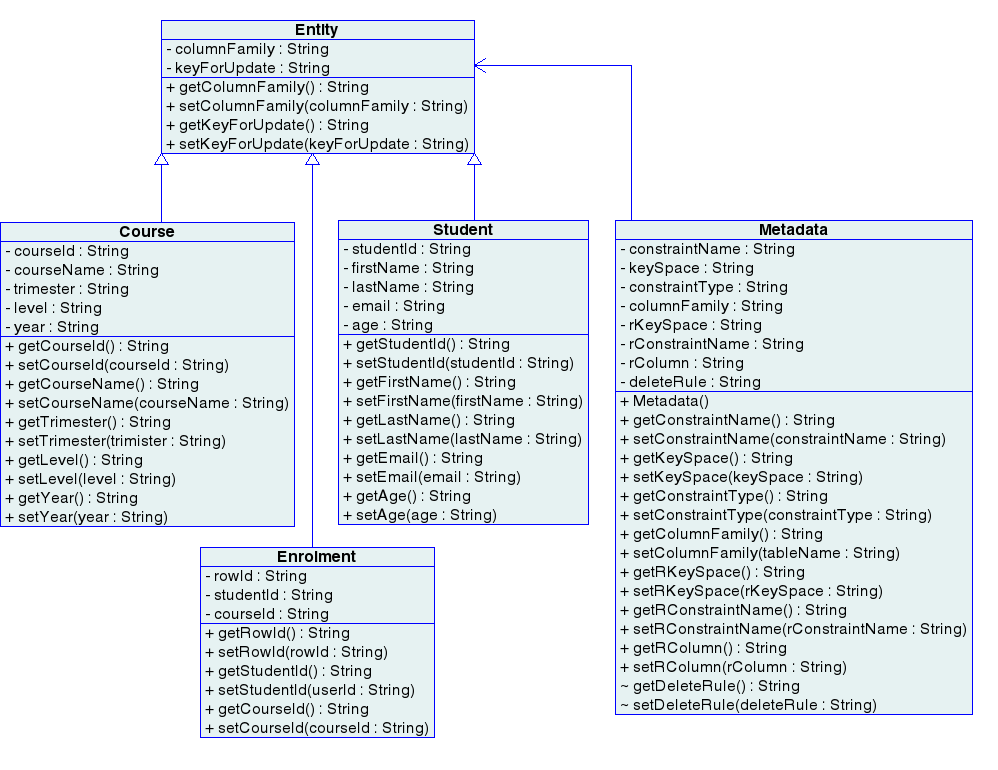
\includegraphics[width=1\textwidth]{./figure/Solutions/classdiagram-experimental.png}
		\caption{Class Diagram for University}\label{fexp:ClassDiagram}
	\end{figure} 

% The constraints for the keyspace are stored in  a  \texttt{Metadata} entity
% class.These constraints are the \ac{PK} and \ac{FK} constraints applicable on each of
% the column families in this keyspace. The list of constraints are the same for
% all the solutions  and are shown in Table~\ref{texp:ListConstraints}.

The list of constraints created for the University keyspace can be seen in
Table~\ref{texp:ListConstraints}. \texttt{CONST100... CONST700} \todo{explain
the purpose of each of them}.


\begin{table}[h] \label{texp:ListConstraints}
\centering
\caption{Metadata}	
	\newcolumntype{C}{@{\hspace{2.5pt}}>{\scriptsize}c@{\hspace{2.5pt}}}
	\begin{tabular}{CCC CCC CC}
		\toprule
		\bfseries ConstraintName & \bfseries Keyspace & \bfseries ConstraintType &
		\bfseries ColumnFamily & \bfseries RKeyspace & \bfseries RConstraintName &
		\bfseries RColumn & \bfseries DeleteRule\\
		\midrule
		CONST100 & University & P & Student & University & & StudentId &\\
		\rc CONST200 & University & P & Course & University & & CourseId &\\
		CONST300 & University & P & Enrolment & University & & RowId &\\
% 		\hline
% 		\hline
		\rc CONST400 & University & R & Enrolment & University & CONST100 & StudentId
		& CASCADE\\
		CONST500 & University & R & Enrolment & University & CONST200 & CourseId &
		NODELETE\\
		\rc CONST600 & University & F & Course & University & CONST500 & CourseId &
		NODELETE\\
		CONST700 & University & F & Student & University & CONST400 & StudentId &
		CASCADE\\
		\bottomrule
	\end{tabular}
\end{table}

% The \texttt{ValidationHandler} in each solution checks these constraints to
% validate referential integrity within this keyspace. The entities are loaded
% generically by the \texttt{EntityManager} for each solution. 
% In the experiment,
% the number of entities inserted for each column family in all the solutions are
% shown in Table~\ref{texp:EntityList}. 
% 	
% 	\begin{table} \label{texp:EntityList}
% 	\centering
% 	\newcolumntype{C} {@{\hspace{2.5pt}}>{\scriptsize}c@{\hspace{2.5pt}}}
% 		\begin{tabular}{CC}
% 			
% 			\toprule
% 			\bfseries ColumnFamily & \bfseries No. of Entities \\
% 			\midrule
% 			Student & 1000 \\
% 			\rc Course & 1000 \\
% 			Enrolment & 10000  \\
% 	% 		\hline
% 	% 		\hline
% 			
% 			\bottomrule
% 		\end{tabular}
% 	\end{table}


\section{Cassandra cluster} \label{sexp:CassandraCluster}
Cassandra is deployed in an homogeneous cluster conformed by 10 nodes. That is,
 all 10 nodes have the same characteristics in software and hardware. These
 nodes emulate a cloud environment in which each node saves
 the data on the local disks of the machines. The characteristics of these nodes
are:


\begin{itemize}
  \item Hardware: \todo{Look on internet the specs of the model}
  	\begin{itemize}
  	  
  	 \end{itemize}
  \item Software: 
  \begin{itemize}
    \item Operating system
    \item Java JDK
    \item Cassandra version
    \item Hector version
  \end{itemize}
\end{itemize}
% Cassandra is deployed in an homogeneous environment The environment to deploy
% cassandra is an homogeneous cluster conformed by 10 nodes. That is, all 10 nodes have the same characteristics in software and
% hardware. These nodes emulate a cloud environment in which each node runs
% Cassandraand saves the data on te local disks of the machines. The
% characteristics of these nodes are:

% 	\begin{table} \label{texp:Nodeconfig}
% 	\centering
% 	\newcolumntype{C} {@{\hspace{2.5pt}}>{\scriptsize}c@{\hspace{2.5pt}}}
% 		\begin{tabular}{CC}
% 			\toprule
% 			\bfseries System configurations\\
% 			\midrule
% 			Linux kernel version & Linux 3.2.4-1-ARCH i686 \\
% 			\rc CPU & Intel(R) Core(TM)2 Duo CPU     E8400  @ 3.00GHz \\
% 			CPU cores & 4  \\
% 			\bottomrule
% 		\end{tabular}
% 	\end{table}
% 
% 
% 
% Linux kernel version: Linux 3.2.4-1-ARCH i686
% 
% CPU: Intel(R) Core(TM)2 Duo CPU     E8400  @ 3.00GHz
% 
% CPU cores: 4


%             total       used       free     shared    buffers     cached
% Mem:          3195       2941        254          0        212       1493

Cassandra configurations:

Version: 0.8.4

Hector Version: 0.8.0-2

Replication strategy:

Partitioner used: Random Partitioner which distrbutes rows in a cluster evenly.
This is the default configuration setting when Cassandra is installed.

The configurations on all the modes are set to the default values in the yaml
configuration file.

The first node is started as a seed node and has the Auto Bootstrap option set
to true. This allows other nodes with this ndoe as its seed to migrate data from
the seed node while data partitioning. For the rest of the nodes tihs options is
set to false.Hinted Handoff is enabled on all nodes.

\begin{itemize}
  \item Hardware
  \item Software
\end{itemize}




%ब
\section{Experimental setup}\label{sexp:ExperimentalSetup}

The experimentation is based on performing \ac{CRUD} operations upon artificial
data created for the University example application. Since it is not a
controlled environment, the experimentation involves performing several runs
where data is inserted, updated, and deleted on the Cassandra cluster. The
environment is not controlled as variables like network latency, parallel
processes in the nodes, and other variables affect the performance.

On each run,  the time required for each operation is recorded in order to assess
its response time for each solution. Additionally,  

 Notice that, each operation on the
artificial data is performed in a batch,   and entities from each column family
are randomly sorted before any operation takes place.  Random sorting is performed in order to
prevent the results to be biased from possible optimization made by Cassandra in
terms of indexes or other criteria. 
		
The artificial data is made up of  students,   courses,  and 
enrolments which is the result of assigning 10 different courses to each
student.  Courses are assigned by dividing the number of courses
into 100 groups of 10 courses each,  and assigning a group for each student. 
Notice that such an assignment involves that X students have the same courses
assigned.  The quantity of records to be inserted for each entity was chosen
considering an overall reasonable time for completing the experimentation of all
solutions. 
		
The format of the artificial data created is as follows.  
	\begin{itemize}
	  
		  \item \texttt{Student} has a
		unit-increasing \texttt{StudentId},  which is merged into the fields \texttt{FirstName}
		 and \texttt{LastName} as "First Name (StudentId)" and "Last Name
		(StudentId)".  \texttt{Email} is composed in a similar way as
		``First. Last@email. (StudentId). com'' and \texttt{Age} is a random number. 
		
		\item  \texttt{Course} has a unit-increasing \texttt{CourseId} which is
		appended to the prefix "COMP".  It also has a composed \texttt{CourseName} as
		in \texttt{Student} (merging id and field).  \texttt{Trimester},  \texttt{Level}
		and \texttt{Year} are randomly generated numbers. 
		
		\item  \texttt{Enrolment} contains a unit-increasing \texttt{RowId},  and the
		respective foreign keys of student and course,  which are \texttt{StudentId}
		and \texttt{CourseId}. 
		
	\end{itemize}

		
The order of the operations performed on the data is as follows.  \textbf{Create}
inserts all the entities for \texttt{Student},  \texttt{Course} and
\texttt{Enrolment}.  \textbf{Update} performs changes on the primary keys of
students and courses,  and on the foreign keys of \texttt{Enrolment} (the one
relative to courses,  specifically).  Finally,  \textbf{Delete} removes all the
\texttt{Student},  \texttt{Course} and \texttt{Enrolment} entities. 
Notice that the primary keys in every column family are different in each run
(create,  update,  delete) in order to avoid introducing biases to the results as
product of the tombstone delete paradigm that Cassandra utilizes.  That is,  since
Cassandra does not completely  remove the primary keys of the inserted entities
(tombstone delete),  reinsertion  using the same primary key might yield faster
times as the key already exists.  After each run,  all column families
(\texttt{Student},  \texttt{Course},  and \texttt{Enrolment}) are emptied and
ready for the next run.   The details  of the \ac{CRUD} operations are explained
further in the following sections. 
		

	
\subsection{Create} The \texttt{Create} operation inserts all the
\texttt{Student},  \texttt{Course} and \texttt{enrolment} entities in that
precise order due to the nature of the referential integrity constraints
presented in Section~\ref{s:ed:ri}.  The time required to insert all of the
entities in their respective column families  is recorded.  In the
\texttt{Student} and \texttt{Course} column families,  \texttt{Create} does not
trigger any referential integrity validation as these entities do not contain
foreign keys. 
Contrarily,  \texttt{Create} on \texttt{Enrolment} triggers foreign key
validation checks on both \texttt{Student} and \texttt{Course} column families. 
		
\subsection{Update} The \texttt{Update} operation is performed after the
creation of all entities. 
First,  an attempt to update the primary key of each \texttt{Course} entity is
made.  This triggers referential integrity validations that result in exceptions
thrown as the \texttt{DeleteRule} for all \texttt{Course} entities is
\texttt{NoDelete}.  Hence,  the times recorded for updating the \texttt{Course}
column family represent the time required to identify a constraint violation and throw
the respective exceptions. 
					
Next,  the \texttt{Enrolment} column family is updated.  In this case,  the
\texttt{CourseId} for each \texttt{Enrolment} entity is changed to a different
one,  ensuring that the distribution of courses and students remains the same. 
The update on the \texttt{Enrolment} column family triggers referential
integrity validation checks to ensure that the course to which every
\texttt{Enrolment} entity is being updated actually exists in \texttt{Course}
column family. 
					
Finally,  the primary key for each \texttt{Student} entity is updated to a new
integer value that previously  never existed in the column family.  Given the
\texttt{Cascade} \texttt{DeleteRule} for \texttt{Student},  this operation
triggers a cascaded update on the
\texttt{Enrolment} column family.  
%  by respectively updating the student foreign
% key,  \texttt{StudentId} in all its existing \texttt{Enrolment} entities. 
All the dependant \texttt{Enrolment} entities of this \texttt{Student} entity
are respectively updated on its foreign key \texttt{StudentId}. 
		
\subsection{Delete} The deletion of entities occurs first on the
\texttt{Enrolment} column family,  where all of its records are deleted without
requiring referential integrity checks as this is a child entity.  The times are
recorded for each \texttt{Delete} operation and then all of the entities are
reinserted with the same primary keys in order to assess the cascaded delete of
\texttt{Student} entities next. 
				
Secondly,  all  the \texttt{Student} entities are deleted from the
\texttt{Student} column family.  Given the \texttt{Cascade} \texttt{DeleteRule} of these entities,  the
\texttt{ValidationHandler} ensures to delete first all of the child entities
before deleting a \texttt{Student} entity. 
Hence,  the times recorded for this operation measure the time required for
performing a cascaded delete on the student dependencies in enrolment.  Notice
that the dependencies exist at this point as they will have been reinserted into
\texttt{Enrolment} in the previous step. 
				
Finally,  all the \texttt{Course} entities are deleted.  Despite the courses
having a \texttt{NoDelete} rule,  notice that at this point the
\texttt{Enrolment} column family is empty,  so courses can be deleted as there
are no child dependencies.  Thus,  the times recorded for this operation measure
referential integrity validation as well as the \texttt{Delete} operation
of the respective entity.  After this final operation,  all column families are
emptied but all the primary keys still exist due to Cassandra's tombstone
delete.  However,  the whole keyspace is ready for the next batch of operations as
the primary keys of all column families will be different. 
	
	



%ब
\section{Performance Indicators} \label{sexp:PerformanceIndicators}
% Performance of database systems is commonly measured in terms of the
% \textit{Response time} and \textit{Throughput}. 

In this thesis,  response time and throughput are the measures used to gauge the
performance of the four solutions while referential integrity validation is
implemented using the \ac{API}. 
Response time refers to the time  a database system takes to process an
operation and produce results to the end user(\todo{cite Demurjian, 
Berkely, serverside, }).  
% Measuring response time for a
% database operation is similar to a black-box evaluation because it is measured 
% without considering the internal functioning  of the database system.  According
% to (\todo{cite Demurjian}) such an evaluation is ideal for a complete database
% system to measure its performance and to give the users details about its 
% efficiency and speed in performing operations.  
Response time for each of the  operations that trigger such a validation from
all the solutions are measured during the experiments. 
This included the time involved to access and retrieve metadata for the entities
and also the time for validating referential integrity by the
\texttt{ValidationHandler}.  
% The response time of Cassandra when such validations
% are not in place is also measured and considered as a baseline with which to
% analyse the solutions.  Such a comparison determines the degree of change in
% speed of Cassandra when such overheads are introduced and gives users useful
% information about how each solution affects the performance of the database
% system. 

The second performance measure used is \textit{Throughput} which is another
classical and commonly used measure of database performance (\todo{cite
BerkleyDB}).  Throughput measures the number of operations processed by the
database system in a unit of time.  In the experiments the throughput of all the
operations triggering referential integrity validation across all solutions is
measured as operations per second.  A single operation stands for each time an
entity is inserted or updated or deleted. Note that only the operations that
introduce the referential integrity validation are measured and thus
\texttt{read} operations are not measured in terms of response time or
throughput. 

% For example,  inserting 1000 students means that 1000 \texttt{insert}
% operations are processed by Cassandra. 
Notice that external variables such as network latency,  simultaneous processes
in the operating systems of each node,  and other variables are not considered
for the analysis of results.  Even when they are present,  it is expected that
results will not be biased by them.  Nonetheless,  the experiments will be
performed at night time over weekends as this is the time when the cluster is
least used,  thus reducing the presence of such variables and hence their impact
by biasing the results. 

In the experiments,  response time and throughput are measured by logging the
time involved to complete each operation in all the solutions. 
For this,  the  real time is recorded before and after every validation.  When all
the iterations of the experiment are completed,  the time
measurements are written to an output log file. 

The traditional TPC benchmarks are not considered as performance measures in
this experiment  because these benchmarks are centred around transactions and
OLTP workloads.  The principal metrics for these benchmarks are the transaction
rate,  query per hour,  cost indicators of a system,  among others,  which are
suitable indicators for \ac{DBMS} with ACID properties~\citep{TPC}.  Hence,  for
assessing Cassandra which lacks SQL queries and  ACID properties,  these
benchmarks are not suitable indicators of performance. 
%  it is
% essential to measure it in terms of what is critical to application  using Cassandra.  In this experiment it is critical to
% measure the difference in time for an operation to complete in Cassandra when
% referential integrity validation is activated or not activated. 


% These operations which trigger referential integrity validation for an entity
% namely the \texttt{insert},  \texttt{update},  \texttt{delete} operations are
% were measured in terms of the throughput in the experiments.  Throughout
% commonly referes to the number of operations performed

% It has to be noted that the operations are prone to  external factors like
% network latency,  bandwidth,  network routing,  network workload among others
% which typically affect a network consisting of several machines and users. 
% This is because the Cassandra cluster used in the experiments is deployed over
% a network that is used by many users concurrently thus exposing the operations
% to such factors.  Identifying such factors and analysing them is beyond the
% scope of this thesis and the analysis is strictly in terms of how the metadata
% storage and referential integrity validation affects Cassandra's performance. 
% It is a general practise for applications to incorporate code within
% applications to log the timestamps for transactions in traditional
% \acp{DBMS}~\citep{IBMPerformance}. 


% In order to determine the response time and throughput,  the output log files are
% are analysed using R.  (\todo{explain how it is imported to R and graphs
% produced--SOS Juan!})





\section{Summary} \label{sexp:Summary} 

This chapter  presented the experimental design to evaluate the performance of
each  solution and the experimental \ac{API} itself using the prototype keyspace
that is used as an example across this thesis.  The experimental design involves
assessing the performance of the CRUD operations on the different solutions
proposed for referential integrity. 
The analysis of results is to be based on response time and throughput,  two
performance indicators that serve as guidelines for assessing the trade-offs
between the different solutions proposed. 
	
	
The next chapter presents the results and their discussions of the experimental
design presented in this chapter
 








% \acresetall
% \section{Cassandra} \label{s:Cassandra}

Cassandra is a distributed data storage system initially developed by Facebook
(\todo{cite BOOK}) for satisfying the needs of large web applications, where
scalability and response time to user requests are critical. It's development is
now undertaken by Apache (Gunda, 2010) and is being used by many large web
applications and large organisations like Facebook, Twitter, Cisco, Digg, Reddit
etc (\todo{cite BOOK}). 

Cassandra is based on the column-oriented key value data model and stores data
in tables that have columns, super column family rows, row keys etc.
These have been explained in Section~\ref{s:key-value-data-model}

Cassandra is run as a single Java process run on a machine and is specifically
designed to work efficiently across different machines and across multiple data
centers, even data centers that are geographically distributed. The details of
the distributed nature is abstracted from  the user and the it appears to the
user that everything is stored on a single machine. This distributed nature
makes Cassandra better utilised when it is run on multiple machines in a cluster
(\todo{Perham, 2010a, BOOK}).

A cluster can be considered as the outermost structure in the data model
of Cassandra. All the machines operating together on which a Cassandra database
relies for holding its data  forms a cluster or ring of nodes
(Figure~\ref{f:cluster}).In such a cluster, all the machines or nodes are
connected to each other and each node is aware of all their peers in the
cluster.

\begin{figure}[h]
	\centering
	%\includegraphics[width=5cm,   height=5cm]{. /figure/random. jpg}
	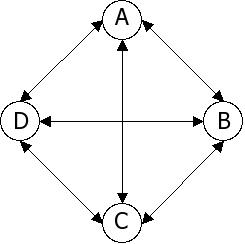
\includegraphics[width=.3\textwidth]{./figure/Solutions/Cassandra-cluster.png}
	\caption{A cluster of nodes in Cassandra}\label{f:cluster}
\end{figure}

Distributed system are prone to conflicts as many users could be issuing
requests on data items from any of the nodes. Any distributed system should
carefully consider conflict resolution and adopt design approaches which would
resolve such conflicts efficiently. Conflicts arise either at read or write operations.
The design approach should either make the system resolve such conflicts either
during one of these operations, deciding the system be either readable at all
times or writable. Cassandra optimises its performance by adopting the design
approach of resolving conflicts during read operations, making Cassandra always
writable.

All nodes in a Cassandra cluster applies the same architectural features
fundamental to Cassandra like bootstrapping, load balancing, replicating and partitioning data,
failure detection mechanisms etc. Some of the key architectural concepts are
explained in the following sub-section.



\subsection{Architecture} \label{ss:Cassandra-architecture}

Cassandra adopts a lot of its architectural concepts from other popular
distributed key-value data storage systems on the cloud, like Google's Bigtable
and Amazon's Dynamo. Overtime these adopted concepts evolved and developed new
features , some of which became specific to Cassandra's architecture. These
architectural concepts gave Cassandra its popular features like elastic
scalability, fault tolerance, high availability and high performance Cassandra's
architecture involves many sophisticated and complex theoretical as well as
mathematical concepts, some of which are discussed below. Discussing every
concept is beyond the scope of this research.

% The nodes in a cluster communicate with each other using the P2P communication
% protocol, Gossip. This protocol involves many complex mathematical models and
% help in significantly reducing the time taken to propagate requests from node to
% node (Raja, 2010).This protocol broadcasts any membership changes to all the
% nodes and allows nodes to reconcile such changes with its peer nodes.
% Using Gossip, nodes thus update their routing information about other nodes
% periodically. This also allows nodes to perform load balancing operations, i.e.,
% some workload is given to other nodes, when a node fails or has a high workload.



\begin{description}
\item[Peer-Peer Distribution Model:] Within a Cassandra cluster, all the nodes
are considered equal or identical in sharing responsibilities and
performing operations, in other words, all nodes are configured as peers and no
single node is a master or slave.  This is unlike traditional\acp{DBMS} that
are distributed, where nodes are configured such that they have different
responsibilities and roles. For example, some or one of the nodes is a master
and others are slaves.
Such a centralised configuration improves reading data, as data can be read from
any of the slave nodes, but write requests are always sent to the master node. This model
thus puts a lot of additional load on the master and also is prone to failure if
the single master node is offline. 

The peer-peer model in Cassandra is decentralized and  provides high data
availability since failure of some of the nodes does not affect the service of
the cluster, as other nodes can carry out the same operation or role. Similarly
this model makes new node additions to the cluster easy. Since nodes are
similar, no specific role has to be assigned to the new nodes, they just have to
be added to the cluster. Addition of nodes invokes the bootstrapping process,
which is explained later.

In a Cassandra cluster nodes use the peer-peer communication protocol called
Gossip for relaying information within the ring. Nodes sent state information at
regular time intervals using the gossiper so that other nodes in the ring can
know their status.

This is essential for failure detection in Cassandra. A gossip session is
initiated with a random node within the cluster during regular intervals where the initiator node  sends a
\texttt{sync} message to another node. If  the recipient node is active it would
return an \texttt{ack} message to the gossiper or the initiator. The initiator
then sends a second \texttt{ack} message to acknowledge the transmission and the
gossip session is completed. If the recipient node does not send an \texttt{ack}
message it is marked as dead and this information is logged.

When a node is found to be offline, after a gossip session, Cassandra implements
the \textit{hinted handoff} feature, to ensure that the operations that were
sent to the failed node are not lost (Figure~\ref{f:hinted handoff}). If a write request
was sent to the failed node, the node that now receives it would create a small
hint message with the information about the write request. This recipient node would use gossip
sessions to check the status of the failed node so that it can give the hint to
the failed node once it is alive again. A hinted handoff acknowledgement is
considered a successful write operation if the consistency level set by the
user, discussed under Eventual Consistency, is low., otherwise it is not
considered as successful and these hinted writes will not be readable. The hinted
handoff feature can be disabled in Cassandra if needed, depending on the suitability of the application using Cassandra.
\begin{figure}[h] 
	\centering
	%\includegraphics[width=5cm,   height=5cm]{. /figure/random. jpg}
	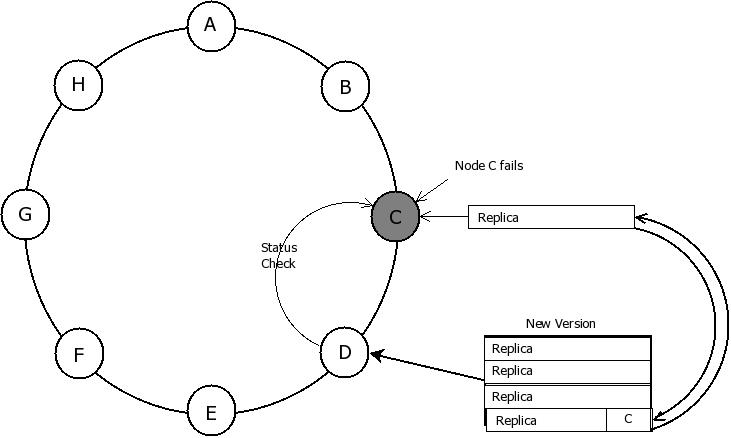
\includegraphics[width=.6\textwidth]{./figure/Solutions/Hinted-handoff.png}
	\caption{Hinted handoff in Cassandra}\label{f:hinted handoff}
\end{figure}

\item[Bootstrapping:] When a node starts for the first time, it checks its
configuration files to retrieve the location information of some of the
initial contact nodes or seed nodes.  It then chooses a random token, which is a
random value, for its position in the cluster and this token information of the
new node is gossiped to the other nodes in the cluster. This enables nodes to
have the routing information of all the peers in a cluster to send requests.
This is illustrated in Figure~\ref{f:bootstrap}, where \texttt{H} is a new node
joining the cluster after checking its configuration files and getting a token to join
the cluster. Its state information is then gossiped through the cluster. Node
\texttt{F} splits its ranges and send it to \texttt{H}, making \texttt{H}
responsible for the keys of that range.

\newpage

\begin{figure}[H]
	\centering
	%\includegraphics[width=5cm,   height=5cm]{. /figure/random. jpg}
	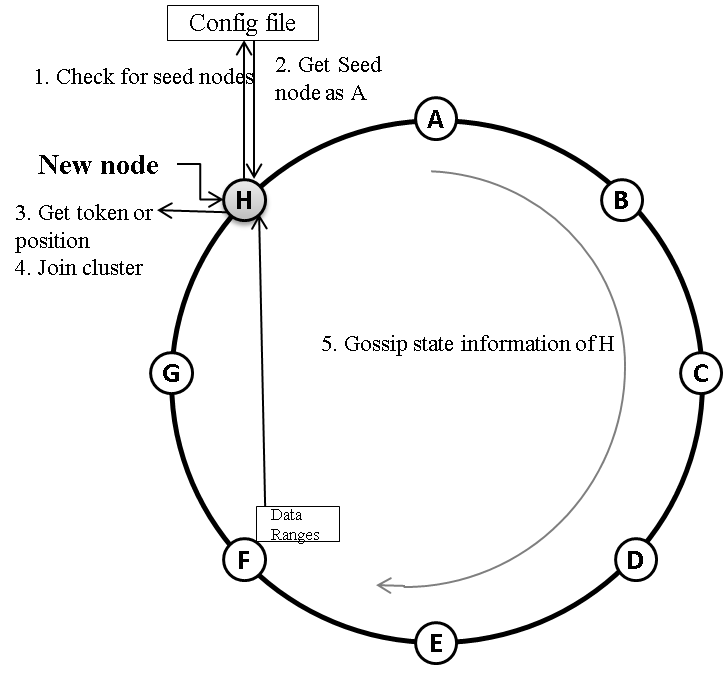
\includegraphics[width=.6\textwidth]{./figure/Solutions/Bootstrapping.png}
	\caption{Bootstrapping in Cassandra}\label{f:bootstrap}
\end{figure}

The token assigned to a new node would help balance the load of an overloaded
node, as some of the operations are transferred to the new node after all nodes
in the cluster know of its existence.  The new node thus is assigned a range
which belonged to another node. The bootstrapping algorithm renders Cassandra
the architectural feature of elastic scalability where adding new nodes is
simple and does not affect other nodes or operations in the cluster. This also helps in load balancing and ensuring that
the cluster has no bottlenecks of overloaded nodes clogging the cluster. To achieve
elastic scalability data has to be dynamically partitioned between the nodes,
which is explained next.

\item[Partitioning Data:] For  elastic scalability and efficient load balancing
Cassandra adopts the consistent hashing used by Amazon's Dynamo to partition
data over the nodes.(\todo{DeCandia et al.(2007)}). In consistent hashing, after
a node is assigned a place in a cluster, data objects that are identifiable by
their keys, are assigned to the node. Each data object's key is hashed and the
data object is sent
to the node that is larger than this hashed value (Figure~\ref{f:consistent
hashing}). This node is called the coordinator node for those keys stored on it.

\begin{figure}[h]
	\centering
	%\includegraphics[width=5cm,   height=5cm]{. /figure/random. jpg}
	\includegraphics[width=.6\textwidth]{./figure/Solutions/Consistent-hashing-Cassandra.png}
	\caption{Consistent hashing in Cassandra}\label{f:consistent hashing}
\end{figure}

Partitioning data helps in load balancing as well as scalability of a cluster to
distribute workload to new nodes without affecting the performance of the
entire cluster. Additionally, in Cassandra better performing nodes are assigned
multiple points in the ring, making them virtual nodes and these nodes are assigned
  workloads from failed nodes or overloaded nodes. 

  \item  [Replication strategy]: For data to be always available to
  the users at all times, irrespective of failures, Cassandra uses a
  replication strategy. This involves replicating every object
  across several nodes by replicating a data item to N number of hosts, where N
  is the number of replicas that the user specifies. After consistent
  hashing, data items are assigned their coordinator nodes and these  nodes
  replicate the assigned objects (DeCandia et al., 2007). After saving the data
  items on locally, the coordinator nodes replicates the data items to N-1
  hosts. A preference list contains routing information about all the
  coordinator nodes that are responsible for storing a key (Figure~\ref{f:
  preference-list})which makes every node in the ring aware of which nodes are
  responsible for a key.
 
\begin{figure}[h]
	\centering
	%\includegraphics[width=5cm,   height=5cm]{. /figure/random. jpg}
	\includegraphics[width=.4\textwidth]{./figure/Solutions/Preference-list.png}
	\caption{A preference list example}\label{f: preference-list}
\end{figure}

Such a replication strategy makes Cassandra highly available as data items are
available from any node in the cluster and node failures do not
affect  data availability. All the nodes would know what ranges of key a
peer node is responsible for from the preference list and this helps in routing
requests to the correct nodes. 

Users can set the level of replication they would prefer, by setting the
replication factor to the number of nodes the users would like to use for
replication. In other words, replication factor tells the cluster how many
copies to save of a single data item. Setting the replication factor to a large
number would help in higher consistency of data items, but replicating data
items to a large number of nodes, each time there is an operation on it,  can
adversely affect the performance.

  \item [Eventual Consistency]:Consistency refers to the ideal scenario where
  all users read the same value of a data item, even when concurrent update
  operations are done on the data item.As mentioned previously, Cassandra opts
  for '\texttt{A}' and '\texttt{P}' of the CAP theorem and allows users to
  determine the level of consistency they would prefer by letting the users set
  the consistency level, which would tell the cluster how many
  replicas should acknowledge operations done on them, for the replicas to be
  considered consistent and up to date. Low consistency levels are considered
  better for performance as higher consistency levels involve more time
  since nodes have to wait to receive acknowledgements from more replicas.
  Letting the users decide the consistency level and replication factor means
  the amount of consistency is ascertained by the users. 

  To ensure the consistency between the nodes that the user sets in the
  consistency level, Cassandra uses the eventual consistency model, which is
  different from the commonly used strict consistency model in traditional
  \acp{DBMS} .
  Strict consistency models ensure that a read operation always returns the most
  update values. This is practical only in situations where the system using
  such a model is dependant on a single machine, where the operations are
  performed sequentially. But in distributed systems, where more machines are
  used, this leads to various conflicts when more than one user is involved. For
  distributed systems a weaker form of consistency, called eventual consistency
  is considered better (\todo{cite BOOK and marked papers}).
  
   Eventual consistency is where every replica agrees to the most recent value
   after a certain point in time and allows updates to be propagated to all the
   replicas asynchronously (Figure~\ref{f: eventual consistency}) (Henry, 2008). Thus, all replicas
   would be consistent eventually after a certain period of time, generally a small number of
   milliseconds \todo{cite book}.
   This requires that the replicas update the values in an order. Eventual
   consistency is useful when a distributed system has to scale greatly.
   If $N$ is the number of nodes containing replicas or the
  replication factor, $W$ is the number of replicas that should
  acknowledge a write operation and $R$ is the number of replicas
  that have to be contacted for a read operation (or the consistency level),
  then eventual consistency can be summarized as:%\\*
  
  \begin{equation}
  	W + R <= N \nonumber  
  \end{equation}
  
  This means that the consistency is not strict as the number of nodes to be
  contacted for a write or read operation is lesser than the number of nodes
  that hold the replicas.
  
  Cassandra performs \textit{read repairs} to make replicas of data consistent
  with the latest versions. Data inconsistencies are determined after checking
  the timestamps of the replicas by the node.  When during a read operation a
  node finds out that the replicas it received from a node  was not consistent with
  replicas on newer nodes, a read repair is performed on the node with the
  outdated replicas. This means that the older
  nodes are sent a write operation with the latest data. 
  
  \begin{figure}[H]
\centering
	% \includegraphics[width=5cm,   height=5cm]{. /figure/random. jpg}
\includegraphics[width=.7\textwidth]{./figure/Solutions/Eventual-consistency-Cassandra.png}
	\caption{Eventual Consistency in Cassandra}\label{f: eventual consistency}
\end{figure}
   This time delay in updating all replicas could translate to latency in a
   large cluster of
  Cassandra nodes, where consistency level and replication factor is high. 
  
% 	  \begin{center}
% 	  \textbf{\texttt{\emph{W} + \emph{R}} \textless = \texttt{\emph{N}}}
% 	  \end{center}
  
  In Cassandra, users have two options while deciding the consistency level:
  single read and the quorum read. In a single read, the first data or replica
  that a node receives from another node is returned as a response to user's
  read request (Figure~\ref{f:singleread}). In a  quorum read, the node that
  receives a read request collects   replicas of data from majority of the available nodes in
  the cluster and returns the most updated data to the user (Figure~\ref{f:quorumread}).
  Quorum reads are slower when compared to single reads, but these prevent stale
  data to be returned.
  
    
  		 \begin{figure}[H]
			\centering
			% \includegraphics[width=5cm,   height=5cm]{. /figure/random. jpg}
			\includegraphics[width=.5\textwidth]{./figure/Solutions/Single-Read-Cassandra.png}
		
			\caption{Single Read in Cassandra}\label{f:singleread}
		\end{figure}
 
		 \begin{figure}[H]
			\centering
			\includegraphics[width=.4\textwidth]{./figure/Solutions/Quorum-read-Cassandra.png}
		
			\caption{Quorum Read in Cassandra}\label{f:quorumread}
		\end{figure}


  
  \item [\ac{SEDA}:] \ac{SEDA} is a concurrency model designed for concurrent
  Internet services, which allows a single operation starting within a single
  thread to let the thread pass the operations to other threads. The work is
  divided into stages, where a stage comprises of an incoming queue, event
  handler and an associated thread pool. This thread pool decides which stages
  to be executed. This is unlike conventional applications where operations are
  run in a single thread. Such a concurrency model helps Cassandra enjoy great
  increase in performance as a stage can be
  controlled by different thread pools that also help in managing the available
  resources like disk space, network bandwidth for the stage to complete the
  work. Work that is divided into stages are mostly the operations like read,
  gossip, load balancing and the like.
  
\end{description}
\subsection{ Write and Read operations}
When users wish to write data into Cassandra tables, they send a write request
to a random node in the cluster (Figure~\ref{f:writeRead}). This node acts as the proxy
and writes the data to the whole cluster, thus efficiently replicating the data.
A user can set the number of nodes that should have the
replicated data copied on it and these replicas are saved on to nodes in the
same data centre and on other nodes in the other data centres. These nodes would act
as proxies when they receive requests from users (Perham, 2010a). This way even
if nodes fail, data is recoverable from other nodes.
		

Similarly, when a user makes a read request to a node, the node acts as a proxy
node and forwards the request to all the other nodes in the cluster
(Figure~\ref{f:singleread}).
As mentioned before, the level of consistency is specified by the user, i.e.,
single or quorum read. Nodes return data to the user after checking the versions
of the replicas and send the latest replica to the user and perform read repairs
on other nodes in the cluster (Perham, 2010b).
The technical details of how to read and write into Cassandra is discussed in
the following chapter.

\begin{figure}[H]
			\centering
			\includegraphics[width=.45\textwidth]{./figure/Solutions/Write-Request-Cassandra.png}
						\caption{A write and read operation in Cassandra}\label{f:writeRead}
		\end{figure}


 
% 
\acresetall
%ब
\chapter{Results and Discussions}
Performance of database systems is commonly measured in terms of the
\textit{Response time} and \textit{Throughput}(\todo{cite Demurjian, Berkely}).
Response time refers to the time  a database system takes to process an
operation and produce results to the end user . Measuring response time for a
database operation is similar to a black-box evaluation because it is measured 
without considering the internal functioning  of the database system. According
to (\todo{cite Demurjian}) such an evaluation is ideal for a complete database
system to measure its performance and to give the users details about its 
efficiency and speed in performing operations. In this thesis, response time and
throughput are the measures used to gauge the performance of Cassandra
while referential integrity validation is implemented using the \ac{API}.

Response time for each of the  operations that trigger such a validation from
all the solutions are measured during the experiments. This included the
time involved to access and retrieve metadata for the entities and also the time for
validating referential integrity by the \texttt{ValidationHandler}. The response
time of Cassandra when such validations are not in place is also measured and considered as a
baseline with which to analyse the solutions. Such a comparison  determines the degree of
change in speed of Cassandra when such overheads are introduced and gives 
users useful information about how each solution affects the performance of
the database system.

The second performance measure used is \textit{Throughput} which
is another classical and commonly used measure of database performance
(\todo{cite BerkleyDB}).
Throughput measures the number of operations processed by the database system in a unit of
time. Across all solutions in the experiments, the throughput for all the
operations triggering referential integrity validation  is measured
as operations per second.
A single operation stands for each time an entity is inserted, updated or
deleted. Note that only the operations that
introduce the referential integrity validation in Cassandra is measured and thus
\texttt{read} operations are not measured in terms of response time or
throughput.

It has to be noted that the operations are prone to  external factors like
network latency, bandwidth, network routing, network workload among others which
typically affect a network consisting of several machines and users. This is
because the Cassandra cluster used in the experiments is deployed over a
network that is used by many users concurrently thus exposing the operations to
such factors. Identifying such factors and analysing them is beyond the scope of
this thesis and the analysis is strictly in terms of how the metadata storage
and referential integrity validation affects Cassandra's performance.

 The results from the experiments were used to
analyse the performance of the four solutions with respect to  response
time and throughput and this is discussed in the following sections.
Section~\ref{sr:baseline} presents the results for the baseline experiment where 
% no referential validation checks are implemented
% and t
the operations performed on the entities are just as it would be performed in
Cassandra. Section~\ref{sr:insert} analyses the results of all the solutions
for the \texttt{insert} operation. Section~\ref{sr:update} presents the analysis
for the \texttt{update} operation for all the solutions. Section~\ref{sr:delete}
discusses the results of the solutions for the \texttt{delete} operation. 






\newcommand{\Width}{0.5\textwidth}
\newcommand{\TB}[1]{\textbf{#1}}

\section{Overview}


\todo{add to tables the unit (seconds, entities per second)}

\todo{Present tables and what they mean}

\todo{Explain why solution 4 is generally better except for update and delete
student}


\subsection{NEW TABLES}
\begin{table}[h]
\centering
\caption{Response time}\label{t:}
\begin{tabular}{ccccccc}
\toprule
&&\textbf{Baseline} & \textbf{Solution1} & \textbf{Solution2} & \textbf{Solution3} & \textbf{Solution4}\\
\midrule
\multirow{3}{*}{\textbf{insert}} & \textbf{s} & 0.088 (0.066) & 0.119 (0.034) & 0.133 (0.013) & 0.422 (0.024) & 0.062 (0.002)\\
 & \textbf{c} & 0.080 (0.038) & 0.111 (0.014) & 0.129 (0.007) & 0.423 (0.032) & 0.061 (0.004)\\
 & \textbf{e} & 0.638 (0.154) & 2.571 (0.238) & 2.727 (0.513) & 6.997 (0.248) & 1.773 (0.082)\\
\midrule
\multirow{3}{*}{\textbf{update}} & \textbf{s} & 0.143 (0.017) & 4.052 (0.471) & 3.982 (0.572) & 9.304 (0.364) & 2.804 (0.080)\\
 & \textbf{c} & 0.143 (0.011) & 0.952 (0.420) & 0.650 (0.014) & 1.354 (0.303) & 0.510 (0.025)\\
 & \textbf{e} & 0.949 (0.306) & 2.710 (0.065) & 2.679 (0.090) & 7.203 (0.218) & 1.964 (0.102)\\
\midrule
\multirow{3}{*}{\textbf{delete}} & \textbf{s} & 0.060 (0.004) & 1.620 (0.411) & 1.749 (0.215) & 5.154 (0.196) & 1.051 (0.149)\\
 & \textbf{c} & 0.053 (0.007) & 0.434 (0.052) & 0.441 (0.012) & 0.770 (0.025) & 0.352 (0.018)\\
 & \textbf{e} & 0.577 (0.046) & 0.850 (0.022) & 1.205 (0.238) & 4.335 (0.250) & 0.569 (0.162)\\
\bottomrule
\end{tabular}
\end{table}



\begin{table}[h]
\centering
\caption{Response time ratio}\label{t:}
\begin{tabular}{ccccccc}
\toprule
&&\textbf{Baseline} & \textbf{Solution1} & \textbf{Solution2} & \textbf{Solution3} & \textbf{Solution4}\\
\midrule
\multirow{3}{*}{\textbf{insert}} & \textbf{s} & 0.09 & 1.34 & 1.51 & 4.78 & 0.70\\
 & \textbf{c} & 0.08 & 1.38 & 1.60 & 5.26 & 0.76\\
 & \textbf{e} & 0.64 & 4.03 & 4.27 & 10.97 & 2.78\\
\midrule
\multirow{3}{*}{\textbf{update}} & \textbf{s} & 0.14 & 28.32 & 27.84 & 65.04 & 19.60\\
 & \textbf{c} & 0.14 & 6.67 & 4.56 & 9.48 & 3.57\\
 & \textbf{e} & 0.95 & 2.85 & 2.82 & 7.59 & 2.07\\
\midrule
\multirow{3}{*}{\textbf{delete}} & \textbf{s} & 0.06 & 27.03 & 29.20 & 86.02 & 17.54\\
 & \textbf{c} & 0.05 & 8.25 & 8.38 & 14.66 & 6.69\\
 & \textbf{e} & 0.58 & 1.47 & 2.09 & 7.51 & 0.99\\
\bottomrule
\end{tabular}
\end{table}






\begin{table}[h]
\centering
\caption{Throughput}\label{t:}
\begin{tabular}{ccccccc}
\toprule
&&\textbf{Baseline} & \textbf{Solution1} & \textbf{Solution2} & \textbf{Solution3} & \textbf{Solution4}\\
\midrule
\multirow{3}{*}{\textbf{insert}} & \textbf{s} & 13582 (3243) & 8802 (1323) & 7556 (600) & 2378 (127) & 16113 (579)\\
 & \textbf{c} & 13717 (2866) & 9114 (839) & 7772 (375) & 2376 (166) & 16455 (1076)\\
 & \textbf{e} & 16212 (2257) & 3918 (302) & 3769 (548) & 1431 (48) & 5652 (241)\\
\midrule
\multirow{3}{*}{\textbf{update}} & \textbf{s} & 7077 (723) & 250 (23) & 255 (27) & 108 (4) & 357 (10)\\
 & \textbf{c} & 7046 (519) & 1212 (369) & 1539 (33) & 761 (101) & 1965 (93)\\
 & \textbf{e} & 11327 (2500) & 3692 (87) & 3737 (124) & 1389 (41) & 5105 (232)\\
\midrule
\multirow{3}{*}{\textbf{delete}} & \textbf{s} & 16754 (1005) & 640 (89) & 578 (53) & 194 (7) & 965 (97)\\
 & \textbf{c} & 19415 (2755) & 2332 (217) & 2271 (61) & 1299 (41) & 2850 (129)\\
 & \textbf{e} & 17424 (1243) & 11773 (301) & 8511 (1084) & 2314 (124) & 18333 (2685)\\
\bottomrule
\end{tabular}
\end{table}



\begin{table}[h]
\centering
\caption{Throughput inverse ratio}\label{t:}
\begin{tabular}{ccccccc}
\toprule
&&\textbf{Baseline} & \textbf{Solution1} & \textbf{Solution2} & \textbf{Solution3} & \textbf{Solution4}\\
\midrule
\multirow{3}{*}{\textbf{insert}} & \textbf{s} & 13582 & 1.54 & 1.80 & 5.71 & 0.84\\
 & \textbf{c} & 13717 & 1.51 & 1.76 & 5.77 & 0.83\\
 & \textbf{e} & 16212 & 4.14 & 4.30 & 11.33 & 2.87\\
\midrule
\multirow{3}{*}{\textbf{update}} & \textbf{s} & 7077 & 28.36 & 27.76 & 65.75 & 19.83\\
 & \textbf{c} & 7046 & 5.82 & 4.58 & 9.26 & 3.59\\
 & \textbf{e} & 11327 & 3.07 & 3.03 & 8.15 & 2.22\\
\midrule
\multirow{3}{*}{\textbf{delete}} & \textbf{s} & 16754 & 26.19 & 28.98 & 86.24 & 17.36\\
 & \textbf{c} & 19415 & 8.33 & 8.55 & 14.94 & 6.81\\
 & \textbf{e} & 17424 & 1.48 & 2.05 & 7.53 & 0.95\\
\bottomrule
\end{tabular}
\end{table}

 
\clearpage
\subsection{OLD TABLES}

\newcolumntype{B}{>{\columncolor{light-gray}}c} 
\begin{table}[h]
 \centering
\caption{Response time}\label{t:}
\begin{tabular}{ccBcccc}
\toprule
&&\textbf{Baseline} & \textbf{Solution1} & \textbf{Solution2} & \textbf{Solution3} & \textbf{Solution4}\\
\midrule
\multirow{3}{*}{\textbf{insert}} & \textbf{s} & 0.624 (0.138) & 0.714 (0.029) &
1.140 (0.057) & 3.444 (0.070) & \TB{0.686 (0.039)}\\
 & \textbf{c} & 0.630 (0.069) & 0.721 (0.027) & 1.181 (0.087) & 3.447 (0.096) &
 \TB{0.684 (0.030)}\\
 & \textbf{e} & 5.708 (0.310) & 16.883 (0.278) & 34.220 (1.399) & 55.359 (0.351)
 & \TB{15.340 (0.276)}\\
\midrule
\multirow{3}{*}{\textbf{update}} & \textbf{s} & 1.254 (0.051) & \TB{32.312
(1.207)} & 67.080 (1.386) & 113.579 (1.495) & 48.000 (1.537)\\
 & \textbf{c} & 1.376 (0.099) & \TB{7.559 (0.297)} & 10.885 (0.384) & 19.279
 (0.252) & 7.580 (0.288)\\
 & \textbf{e} & 7.237 (0.425) & 18.228 (0.276) & 35.673 (1.402) & 56.762 (0.420)
 & \TB{16.694 (0.386)}\\
\midrule
\multirow{3}{*}{\textbf{delete}} & \textbf{s} & 0.592 (0.022) & \TB{10.798
(0.409)} & 18.952 (0.600) & 42.544 (0.619) & 35.919 (0.576)\\
 & \textbf{c} & 0.627 (0.023) & 3.602 (0.092) & 4.828 (0.118) & 6.745 (0.120) &
 \TB{3.324 (0.079)}\\
 & \textbf{e} & 5.847 (0.294) & 5.904 (0.359) & 12.282 (0.650) & 35.070 (0.472)
 & \TB{5.879 (0.240)}\\
\bottomrule
\end{tabular}
\end{table}



\begin{table}[h]
 \centering
\caption{Response time ratio}\label{t:}
\begin{tabular}{ccBcccc}
\toprule
&&\textbf{Baseline} & \textbf{Solution1} & \textbf{Solution2} & \textbf{Solution3} & \textbf{Solution4}\\
\midrule
\multirow{3}{*}{\textbf{insert}} & \textbf{s} & 0.62 & 1.14 & 1.83 & 5.52 &
\TB{1.10}\\
 & \textbf{c} & 0.63 & 1.14 & 1.87 & 5.47 & \TB{1.09}\\
 & \textbf{e} & 5.71 & 2.96 & 6.00 & 9.70 & \TB{2.69}\\
\midrule
\multirow{3}{*}{\textbf{update}} & \textbf{s} & 1.25 & \TB{25.76} & 53.48 &
90.55 & 38.27\\
 & \textbf{c} & 1.38 & \TB{5.49} & 7.91 & 14.01 & 5.51\\
 & \textbf{e} & 7.24 & 2.52 & 4.93 & 7.84 & \TB{2.31}\\
\midrule
\multirow{3}{*}{\textbf{delete}} & \textbf{s} & 0.59 & \TB{18.24} & 32.02 &
71.88 & 60.68\\
 & \textbf{c} & 0.63 & 5.74 & 7.70 & 10.76 & \TB{5.30}\\
 & \textbf{e} & 5.85 & 1.01 & 2.10 & 6.00 & \TB{1.01}\\
\bottomrule
\end{tabular}
\end{table}






\begin{table}[h]
 \centering
\caption{Throughput}\label{t:}
\begin{tabular}{ccBcccc}
\toprule
&&\textbf{Baseline} & \textbf{Solution1} & \textbf{Solution2} & \textbf{Solution3} & \textbf{Solution4}\\
\midrule
\multirow{3}{*}{\textbf{insert}} & \textbf{s} & 1634 (157) & 1403 (56) & 880
(41) & 290 (6) & \TB{1463 (71)}\\
 & \textbf{c} & 1598 (108) & 1389 (52) & 851 (61) & 290 (7) & \TB{1465 (62)}\\
 & \textbf{e} & 1756 (70) & 592 (9) & 293 (12) & 181 (1) & \TB{652 (11)}\\
\midrule
\multirow{3}{*}{\textbf{update}} & \textbf{s} & 798 (30) & \TB{31 (1)} & 15 (0)
& 9 (0) & 21 (1)\\
 & \textbf{c} & 730 (43) & \TB{132 (5)} & 92 (3) & 52 (1) & 132 (5)\\
 & \textbf{e} & 1385 (62) & 549 (8) & 281 (11) & 176 (1) & \TB{599 (13)}\\
\midrule
\multirow{3}{*}{\textbf{delete}} & \textbf{s} & 1692 (61) & \TB{93 (3)} & 53 (2)
& 24 (0) & 28 (0)\\
 & \textbf{c} & 1597 (57) & 278 (7) & 207 (5) & 148 (3) & \TB{301 (7)}\\
 & \textbf{e} & 1714 (80) & 1700 (95) & 817 (45) & 285 (4) & \TB{1704 (64)}\\
\bottomrule
\end{tabular}
\end{table}



\begin{table}[h]
\newcommand{\B}[1]{\colorbox{light-gray}{#1}}
 \centering
\caption{Throughput inverse ratio}\label{t:}
\begin{tabular}{ccBcccc}
\toprule
&&\textbf{Baseline} & \textbf{Solution1} & \textbf{Solution2} & \textbf{Solution3} & \textbf{Solution4}\\
\midrule
\multirow{3}{*}{\textbf{insert}} & \textbf{s} & 1634 & 1.17 & 1.86 & 5.63 &
\TB{1.12}\\
 & \textbf{c} & 1598 & 1.15 & 1.88 & 5.51 & \TB{1.09}\\
 & \textbf{e} & 1756 & 2.96 & 6.00 & 9.72 & \TB{2.69}\\
\midrule
\multirow{3}{*}{\textbf{update}} & \textbf{s} & 798 & \TB{25.77} & 53.54 & 90.67
& 38.29\\
 & \textbf{c} & 730 & \TB{5.51} & 7.93 & 14.06 & 5.52\\
 & \textbf{e} & 1385 & 2.52 & 4.93 & 7.86 & \TB{2.31}\\
\midrule
\multirow{3}{*}{\textbf{delete}} & \textbf{s} & 1692 & \TB{18.24} & 32.03 &
71.96 & 60.75\\
 & \textbf{c} & 1597 & 5.75 & 7.71 & 10.77 & \TB{5.31}\\
 & \textbf{e} & 1714 & 1.01 & 2.10 & 6.01 & \TB{1.01}\\
\bottomrule
\end{tabular}
\end{table}





\newpage
\section{Insert}

	\subsection{Student}
		\begin{figure}[H]
			\subfigure[Response time]
			{\includegraphics[width=\Width]{figure/result/barplot-insert_student-rt.pdf}}
			\subfigure[Throughput]
			{\includegraphics[width=\Width]{figure/result/barplot-insert_student-tp.pdf}}
			\caption{Performance inserting students}\label{f:rd:insert-user}
		\end{figure}
\newpage
	\subsection{Course}
		\begin{figure}[H]
			\subfigure[Response time]
			{\includegraphics[width=\Width]{figure/result/barplot-insert_course-rt.pdf}}
			\subfigure[Throughput]
			{\includegraphics[width=\Width]{figure/result/barplot-insert_course-tp.pdf}}
			\caption{Performance inserting courses}\label{f:rd:insert-course}
		\end{figure}	
\newpage	
	\subsection{Enrolment}
		\begin{figure}[H]
			\subfigure[Response time]
			{\includegraphics[width=\Width]{figure/result/barplot-insert_enrolment-rt.pdf}}
			\subfigure[Throughput]
			{\includegraphics[width=\Width]{figure/result/barplot-insert_enrolment-tp.pdf}}
			\caption{Performance inserting enrolments}\label{f:rd:insert-enrolment}
		\end{figure}
		
\clearpage
\newpage
\section{Update}

	\subsection{Student}
		\begin{figure}[H]
			\subfigure[Response time]
			{\includegraphics[width=\Width]{figure/result/barplot-update_student-rt.pdf}}
			\subfigure[Throughput]
			{\includegraphics[width=\Width]{figure/result/barplot-update_student-tp.pdf}}
			\caption{Performance updating students}\label{f:rd:update-user}
		\end{figure}
\newpage	
	\subsection{Course} 
		\begin{figure}[H]
			\subfigure[Response time]
			{\includegraphics[width=\Width]{figure/result/barplot-update_course-rt.pdf}}
			\subfigure[Throughput]
			{\includegraphics[width=\Width]{figure/result/barplot-update_course-tp.pdf}}
			\caption{Performance updating courses}\label{f:rd:update-course}
		\end{figure}	
\newpage	
	\subsection{Enrolment}
		\begin{figure}[H]
			\subfigure[Response time]
			{\includegraphics[width=\Width]{figure/result/barplot-update_enrolment-rt.pdf}}
			\subfigure[Throughput]
			{\includegraphics[width=\Width]{figure/result/barplot-update_enrolment-tp.pdf}}
			\caption{Performance updating enrolments}\label{f:rd:update-enrolment}
		\end{figure}
\clearpage
\newpage
\section{Delete} 

	\subsection{Student}
		\begin{figure}[H]
			\subfigure[Response time]
			{\includegraphics[width=\Width]{figure/result/barplot-delete_student-rt.pdf}}
			\subfigure[Throughput]
			{\includegraphics[width=\Width]{figure/result/barplot-delete_student-tp.pdf}}
			\caption{Performance deleting students}\label{f:rd:delete-user}
		\end{figure} 
\newpage	  
	\subsection{Course}
		\begin{figure}[H]
			\subfigure[Response time]
			{\includegraphics[width=\Width]{figure/result/barplot-delete_course-rt.pdf}}
			\subfigure[Throughput]
			{\includegraphics[width=\Width]{figure/result/barplot-delete_course-tp.pdf}}
			\caption{Performance deleting courses}\label{f:rd:delete-course}
		\end{figure}	
\newpage	 
	\subsection{Enrolment}
		\begin{figure}[H]
			\subfigure[Response time]
			{\includegraphics[width=\Width]{figure/result/barplot-delete_enrolment-rt.pdf}}
			\subfigure[Throughput]
			{\includegraphics[width=\Width]{figure/result/barplot-delete_enrolment-tp.pdf}}
			\caption{Performance deleting enrolments}\label{f:rd:delete-enrolment}
		\end{figure}
		


	
% 
% % 
% \acresetall
% %ब 
\chapter{Results and Discussions}
% The results and discussion for each solution considers the time taken for
% operations to complete on each of the entities  as described in the University
% example adopted for the experiments.

% Performance of database systems is commonly measured in terms of the
% \textit{Response time} and \textit{Throughput}(\todo{cite Demurjian, Berkely}).
% Response time refers to the time  a database system takes to process an
% operation and produce results to the end user . Measuring response time for a
% database operation is similar to a black-box evaluation because it is measured 
% without considering the internal functioning  of the database system. According
% to (\todo{cite Demurjian}) such an evaluation is ideal for a complete database
% system to measure its performance and to give the users details about its 
% efficiency and speed in performing operations. In this thesis, response time and
% throughput are the measures used to gauge the performance of Cassandra
% while referential integrity validation is implemented using the \ac{API}.
% 
% Response time for each of the  operations that trigger such a validation from
% all the solutions are measured during the experiments. This included the
% time involved to access and retrieve metadata for the entities and also the time for
% validating referential integrity by the \texttt{ValidationHandler}. The response
% time of Cassandra when such validations are not in place is also measured and considered as a
% baseline with which to analyse the solutions. Such a comparison  determines the degree of
% change in speed of Cassandra when such overheads are introduced and gives 
% users useful information about how each solution affects the performance of
% the database system.
% 
% The second performance measure used is \textit{Throughput} which
% is another classical and commonly used measure of database performance
% (\todo{cite BerkleyDB}).
% Throughput measures the number of operations processed by the database system in a unit of
% time. In the experiments the throughput for all the operations
% triggering referential integrity validation across all solutions is measured
% as operations per second.
% A single operation stands for each time an entity is inserted or updated or
% deleted. 
% % For example, inserting 1000 students means that 1000 \texttt{insert}
% % operations are processed by Cassandra. 
% Note that only the operations that
% introduce the referential integrity validation in Cassandra is measured and thus
% \texttt{read} operations are not measured in terms of response time or
% throughput.
% % These operations
% % which trigger referential
% % integrity validation for an entity
% % namely the \texttt{insert}, \texttt{update}, \texttt{delete} operations are
% % were measured in terms of the throughput in the experiments. Throughout commonly
% % referes to the number of operations performed
% 
% It has to be noted that the operations are prone to  external factors like
% network latency, bandwidth, network routing, network workload among others which
% typically affect a network consisting of several machines and users. This is
% because the Cassandra cluster used in the experiments is deployed over a
% network that is used by many users concurrently thus exposing the operations to
% such factors. Identifying such factors and analysing them is beyond the scope of
% this thesis and the analysis is strictly in terms of how the metadata storage
% and referential integrity validation affects Cassandra's performance.

 The results from the experiments were used to
analyse the performance of the four solutions with respect to  response
time and throughput and this is discussed in the following sections.
Section~\ref{sr:baseline} presents the results for the baseline experiment where 
% no referential validation checks are implemented
% and t
the operations performed on the entities are just as it would be performed in
Cassandra. Section~\ref{sr:insert} analyses the results of all the solutions
for the \texttt{insert} operation. Section~\ref{sr:update} presents the analysis
for the \texttt{update} operation for all the solutions. Section~\ref{sr:delete}
discusses the results of the solutions for the \texttt{delete} operation. 


\section{Baseline}\label{sr:baseline}
The performance of Cassandra when referential
integrity validation is introduced using any of the solutions is compared with a
a base experiment where the operations on the entities do not trigger any
such validations. Such a baseline is useful to determine the
performance of the database system when validations are imposed using the
\ac{API} and to analyse the performance of the solutions.
% baseline experiment has no referential integrity validation introduced and
In the baseline experiment, the operations on the entities represent how
data is inserted into Cassandra without referential integrity validations. The
results in terms of response time for the baseline experiment is presented as
a bar-plot in Figure~\ref{fr:Solution0-barplot}. The analysis of
the performance of each operation on an entity is discussed as follows.
% The results are analysed in the
% following 

% The factors measured were the time involved to complete each operation for every
% entity, where the operations considered were the ones that invoked referential
% integrity validation, namely, \texttt{insert}, \texttt{update} and
% \texttt{delete}. These were measured for the entities in the University example,
% namely \texttt{Student}, \texttt{Course} and \texttt{Enrolment}.
% The results are plotted as a histogram in Figure~\ref{}
	
\begin{figure}[h] \centering
\includegraphics[width=.8\textwidth]{./figure/result/Solution0-barplot.png}
		\caption{Baseline}\label{fr:Solution0-barplot}
	\end{figure}
	
% Present results.
% 	The potential reasons for the variance of time for the completion of each
% 	operations on the different entities are summarised next.
	\begin{description}
	\item[Insert] The results from the baseline experiment show that the time for
	inserting entities into the \texttt{Student} and \texttt{Course} column families 
	are similar. This is because the number of entities inserted into these
	column families are exactly the same.
% 	\texttt{1000} instances of \texttt{Student} and \texttt{Course} are inserted
% 	into the respective column families in the baseline experiment. 
	The time taken
	to insert the \texttt{Enrolment} entities into the \texttt{Enrolment} column family
	is higher by approximately \texttt{4} seconds. This is because
	\texttt{Enrolment} has more entities than the other column families, to be
	specific it has \texttt{10,000} instances which is 10 times more entities than
	\texttt{Student} and \texttt{Course}.
% 	Hence, the \texttt{insert} operation takes more time to insert entities into \texttt{Enrolment} column family, especially considering its
% 	replication across \texttt{10} nodes, which would add to the time in
% 	completing the operation.
	
	\item[Update] The time for updating the primary keys in \texttt{Student} and
	\texttt{Course} are comparable to each other. Although the number of entities
	updated are the same, the small difference is owing to external variables
	(e.g. network latency, high network traffic). Similar to the \texttt{insert}
	operation, updating the \texttt{Enrolment} entities takes significantly more
	time, which is again due to the higher number of entities held within this
	column family. 
	
	The  response time of the \texttt{update} operation on
	\texttt{Enrolment} is higher when compared to the response  time of
	\texttt{insert} operation on the same. This is mainly due to the additional
	computational resources consumed to ensure the existence of an entity before
	updating it to new values.
	
	\item[Delete] The time involved for completion of the \texttt{delete} operation
	on all the entities from \texttt{Student} and \texttt{Course} column families
	are similar to each other owing to the same number of entities. The time
	involved for the \texttt{delete} operation to delete all the entities in
	\texttt{Enrolment} is higher just as in other operations. This is again due to
	the larger number of entities present in \texttt{Enrolment}.
	
	Performance of the \texttt{delete} operation is similar to the\texttt{insert}
	operation in terms of time taken for completion and the processes involved. This
	means that unlike \texttt{update} both \texttt{delete} and \texttt{insert} do
	not involve additional operations and simply adds or removes entities from the
	column families. It should also be noted that external factors affect the
	performance of the operations.
	
	\end{description} 

	
	
% 	Explain Insert. Why student and course similar. Why enrolment much higher.
% 	

	In general, all the operations take more time to complete on the
	\texttt{Enrolment} column family due to its larger number of entities 
	when compared to \texttt{Student} and \texttt{Course} column families. The
	\texttt{update} operation consumes more time due to the additional search
	involved to locate the previous state of the entity prior to updating it to new
	values. Notice that the time involved to complete \texttt{insert} and
	\texttt{delete} entities form all the three column families are similar.
	
	The following sections analyse the performance of each solution  in
	terms of how its referential integrity validation in each of the
	\texttt{insert}, \texttt{update} and \texttt{delete} operation and its
	metadata storage affect the performance.
	
\section{Insert}\label{sr:insert}
An \texttt{insert} operation triggers a referential integrity validation
whenever a child entity containing foreign keys is inserted where the
\texttt{ValidationHandler} validates that the foreign keys exist as primary keys in the parent
entities. 
% This dependency information is retrieved from the metadata saved in
% each solutions. 
In the experiments, the time taken to insert all the
entities are recorded thus also measuring the time involved for validating
referential integrity for each entity. Across all the solutions in the
experiments, the \texttt{insert} operation triggers such a validation when the
\texttt{Enrolment} entities are inserted since it is a child entity containing
foreign keys of \texttt{Student} and \texttt{Course} entities.
%  As mentioned in
% Section~\ref{s:exp:setup} the number of entities inserted into the
% \texttt{Enrolment} column family is the same for all solutions and the baseline
% experiment.
% Despite the same number of entities and similar validation performed, 
The response time and throughout of the \texttt{insert} operation in all the
solutions and the baseline experiment are plotted in
Figure~\ref{fr:insert-result}.
% 	\begin{figure}[H] \centering
% 	\includegraphics[width=.8\textwidth]{./figure/result/op-insert-barplot.png}
% 		\caption{}\label{fr:response-insert}
% 	\end{figure}
	
	
	
	
	
	
	
	
The results of all the solutions as seen in Figure~\ref{fr:insert-result} with
respect to response time  is discussed as follows based on the different
entities on which the \texttt{insert} operation is applied.
\subsection{Response Time}
\begin{itemize}
  \item The results show that the response time of all
  the solutions to insert entities into \texttt{Student} and \texttt{Course}
  column families is similar and always lesser than 5 seconds. This is because
  no referential integrity validation is invoked when parent entities are
  inserted as these do not contain any foreign keys. Note that the metadata for
  any entity is accessed and checked by the \texttt{ValidationHandler}
  to determine if it has dependencies or not. It is during this
  check that it is determined if an entity is a parent or child. 
  So across all solutions even when parent entities \texttt{Student} and
  \texttt{Course} are inserted their metadata is accessed.
  
  Solutions~1, 2  and 4 have approximately similar response times since the metadata 
  access for these solutions are easier as metadata is a part of the entity and 
  no additional connection to a metadata column family is required. Solution~3
  takes slightly longer than the rest of the solutions and this is because of the way
  the metadata is accessed for the entities in this solution. 
% irrespective of whether an entity is a parent or child the
% \texttt{ValidationHandler} performs the same check the metedata of the entity
% for all the solutions. It is when this check is made it is clear if the entity
% is a parent or child. 
  In this solution accessing the metadata for every 
  \texttt{Student} and \texttt{Course} entity causes the slower
  response time since a different \texttt{Metadata} column family has to be
  accessed using the connection object. This is because metadata is not cached
  for re-use in this solution. Unlike this, Solution~4 caches  metadata for
  entities and re-uses it thus saving time by not having to access a separate
  column family for each entity insertion.
  
  When compared to the baseline experiment the insertion of parent entities
  in all the solutions, except Solution~3, take similar response times despite
  the initial metadata access. Solution~3 takes only a few seconds
  longer to complete the operation when compared to the baseline.
  


  \item The response time involved for inserting the \texttt{Enrolment}
  entities differs across solutions. Since these entities have existing \ac{FK}
  constraints in their metadata indicating they are dependent on a parent
  entity, referential integrity validations are triggered. The results in
  Figure~\ref{fr:insert-result} show that Solutions~1 and 4 take approximately 15 seconds to
  insert  \texttt{Enrolment}entities and take the least time when compared
  to the other solutions.  Solution~2 takes lesser than 35 seconds while
  Solution~3 takes longer than the rest of the solutions 
  This is mainly due to the way metadata is accessed and read from  a different
  \texttt{Metadata} column family in this solution. In the rest of the solutions the 
  metadata is either a part of the entity, making the access easier or it is
  cached as in Solution~4 thus requiring no extra connections to a column family. 
  
  As seen in the baseline experiment inserting \texttt{Enrolment} entities  has
  a higher response time in the solutions. But the response time for this
  operation on \texttt{Enrolment} is higher in the solutions when compared to
  the baseline experiment. This means that referential integrity validation in
  each solution increases the response time slightly, depending on the way the
  metadata is accessed for the entities in the solutions. Moreover, the entities
  inserted into the \texttt{Enrolment} column family is ten times more than the
  other column families.
% The validation involves accessing the columns of the  column family in this
% solution to get each value of the constraint.
\end{itemize}

Generally, the response time for inserting child entities is higher across the
solutions when compared to the response time for inserting parent entities. In
the baseline experiment this was solely because of the larger number of entities
in the child entity class, while in the solutions it was due to the referential
validation triggered while inserting child entities and also the larger number
of entities. Inserting parent entities is similar in the baseline
experiment and the solutions despite the metadata access present in the
solutions. This is so because no additional validations are triggered in the
solutions. 


\subsection{Throughput}

To summarise this operation, the results show that Solutions~1 and 4 perform
similarly with respect to inserting child and parent entities and are faster
 than the rest of the solutions while Solution~3 is the slowest for both the
 cases. the different response times for the solutions are owing to the
 different styles of metadata storage as explained previously.

%  It can be that the response time  
%  On the other hand, Solution~4 caches the metadata information for entities and
%  does not need to connect to the metadata column family each time any operaion
%  is triggered on an entity. Solutions~1 and 2 take approximately the same time
%  and the metadata access for these solutions are easier as it comes as a part of
%  the entity and no additional connetion to the metadata is required. 
%  
% 
% On the other hand the time consumed to insert \texttt{Enrolment} entities varies
% across the solutions since there is referential integrity validation where
% metadata constraints are read and validated.

		
% Performing the \texttt{insert} operation for the 10000 entities in
% \texttt{Enrolment} is thus more time consuming for all the solutions when
% compared to inserting entities into other column families and this is similar to
% the baseline experiment where inserting \texttt{Enrolment} entities was more
% time consuming.
% However in the solutions, the time taken to insert entities into
% \texttt{Enrolment} is higher when compared to the same in the baseline tests and
% this is  due to the referential validation that is triggered while inserting
% child entities in the solutions. 
\newpage

\newcommand{\Width}{.8\textwidth}
	\begin{figure}[H] \label{fr:insert-result}
		\centering
		\subfigure[Response Time]{
			\includegraphics[width=\Width]{./figure/result/op-insert-barplot.png}
% 			\caption{Response Time for \texttt{insert}}\label{fr:response-insert}
		}
		\subfigure[throughput]{
			\includegraphics[width=\Width]{./figure/result/th-insert-barplot.png}
% 			\caption{Throughput}\label{fr:through-insert}
		} 
	\caption{Response time and Throughput of \texttt{insert} operation}
	\end{figure}

\section{Update}\label{sr:update}
In all the solutions, the \texttt{update} operation triggers a referential
integrity validation whenever an entity is updated with new values. 
% Moreover,
% data manipulation rules are also applied which specifies whether the \texttt{update} is a
% \texttt{Cascade} or \texttt{NoDelete}. 
The \texttt{ValidationHandler} in all the
solutions perform these validations and accesses metadata and its various parts
to determine whether referential integrity is violated or not. This is
unlike the baseline experiment where  no referential integrity
validations  are performed and entities are updated without
checking its correctness or validity. 

In all the solutions the time taken to update the primary keys in
\texttt{Student} and \texttt{Course} column families and the time taken to
update the foreign key \texttt{CourseId} in \texttt{Enrolment} is measured
in terms of response time and throughput. The
results are presented in Figure~\ref{fr:update-result} and the performance of
the solutions in an \texttt{update} is discussed next.

	\begin{figure}[h] \label{fr:update-result}
		\centering
		\subfigure[Response Time]{
			\includegraphics[width=\Width]{./figure/result/op-update-barplot.png}
% 			\caption{Response Time for \texttt{insert}}\label{fr:response-insert}
		}
		\subfigure[Throughput]{
			\includegraphics[width=\Width]{./figure/result/th-update-barplot.png}
% 			\caption{Throughput}\label{fr:through-insert}
		} 
	\caption{Response time and Throughput of \texttt{insert} operation}
	\end{figure}
	
	\subsection{Response Time}
	The response time of the solutions based on the results fro the experiments are
	analysed and is categorised on the different cases applicable in the
	\texttt{update} operation. The different cases are a cascaded
	and \texttt{NoDelete} \texttt{update} operations on primary keys and 
	the foreign key updates in child entities.
	
	
	\begin{itemize}
	  \item The \texttt{update} operation on \texttt{Student} entities is
	  cascaded since the \texttt{DeleteRule} for \texttt{Student} is
	  \texttt{Cascade} . Note that for the cascaded \texttt{update} operation
	  the dependent values in \texttt{Enrolment} is also updated, 
	  which incurs additional time for this operation to complete.
% 	  Updating \texttt{Student} entities involve cascading
% 	  the changes within the child entity \texttt{Enrolment}.
% 	%  while updating \texttt{Course} throws an
	% exception since \texttt{course} entities have a \texttt{NoDelete} manipulation
	% rule in its metadata, thus preventing the \texttt{update}. 
	The results in Figure~\ref{fr:update-result} show that all the solutions have
	different response times for updating \texttt{Student} entities.
	Solution~2 takes the least time to perform the updates when compared to the
	other solutions while Solution~1 takes approximately 10 seconds more than
	Solution~2.(\todo{check update of Sol2}) Solution~3 has the highest response
	time of 100 seconds and this is because for each \texttt{update} operation
	on \texttt{Student} entities, the metadata column family in this solution is
	accessed and the metadata is processed each time by the
	\texttt{ValidationHandler} to validate referential integrity. Solution~4 is
	faster than Solution~3 mainly because it caches the metadata for the entity
	class and uses the cached metadata for all the entities of the entity class.
	This helps in saving time as \texttt{ValidationHandler} does not have to access
	a separate column family for each operation.  
	% slightly more than 25 seconds to
	% perform a cascaded \texttt{update} for \texttt{Student} entities.
	But Solution~4 takes longer than Solutions~1 and 2 because despite the cached
	metadata it has to initially fetch the metadata from an external location unlike
	the latter solutions. 
	% olution~2 takes slightly more than 20 seconds and takes
	% lesser time than other solutions, while Solution~3 takes the most time of more than 60 seconds. 
	All the solutions takes more time to insert \texttt{Student} entities when compared to
	the baseline due to the referential integrity validation and the cascaded
	operations, which additionally accesses \texttt{Enrolment} to complete the
	\texttt{update} operation. The difference in response time when referential
	integrity validation is in place and when it is not in the baseline experiment
	ranges from more than 20 seconds to above 100 seconds.
	
	  \item Updating \texttt{Course} entities involves identifying the metadata
	constraints and raising an exception due to the \texttt{NoDelete} rule applicable for every
	\texttt{Course} entity. From the
	results in Figures~\ref{fr:update-result} it can inferred that both Solutions~1 and 4 take
	the least time amongst all solutions to insert \texttt{Course} entities. These
	solutions take least time since for the former the metadata is easily accessed
	being a part of the entity thus not requiring additional accessing time.
	Solution~4 access the entity metadata from the cached metadata maintained in
	this solution, making it faster to fetch the metadata for all entities of a
	particular entity class. 
% 	where Solution~1 takes less than 5 seconds and
% 	Solution~4 close to it.
	Solution~2 is not far behind form these solutions and
	takes slightly more than 5 seconds. This is because in Solution~2 the metadata
	is accessed for each entity after searching for the top row incurring some
	additional time every time an entity is updated. Solution~3 takes nearly twice
	the amount of time than the rest of the solutions for this operation. Just as
	in updating \texttt{Student} entities this is due to the separate access
	required to the \texttt{Metadata} column family and identifying the appropriate constraints for an entity class in it. 
	
	When compared to the baseline, updating \texttt{Course} takes more time in all
	solutions since  validations are triggered and  exceptions are raised unlike
	the baseline. The only difference between this operation in the solutions and the
	baseline experiment is the time involved in accessing the metadata and
	determining the \texttt{DeleteRule} and handling the exceptions.
	
	\item When \texttt{Enrolment} entities are  updated the changes are applied
	only within the
	\texttt{Enrolment} column family although \texttt{Student} and
	\texttt{Course} column families are accessed to ensure the new
	foreign keys exist. The results in Figure~\ref{fr:update-result} show that
	Solutions~1 and 4 almost take almost the same time. This is similar to the
	\texttt{update} on \texttt{course} entities and is because of the way the
	metadata is accessed and used by the \texttt{ValidationHandler}. 
	Solution~2 takes slightly more than Solutions~1 and 4 because of the way it
	has to search for the top row to identify the entities metadata each time.
	As seen in previous cases, Solution~3 takes the highest time and this is owing
	to the separate access to \texttt{Metadata}. column family.
	
	When compared to the baseline experiment, the solutions are slower because
	parent column families are accessed always  to check the existence of the new
	values in every validation by the \texttt{ValidationHandler}. 
	\end{itemize}
	
Generally, in all the solutions updating the \texttt{Course} entities take the
least time when compared to updating \texttt{Student} or \texttt{Course}
entities. This is because although \texttt{update} on \texttt{Course} entities trigger
validation, the entities are not updated and neither are any cascade operations
performed.
The time involved in updating \texttt{Students} is higher than updating the
\texttt{Enrolment} entities due to the cascading operations  and
the changes made in child column families.
Moreover for \texttt{update} on \texttt{Enrolment} the validation is limited to
accessing the parent entities to ensure the existence of the foreign keys.
The \texttt{update} on \texttt{Enrolment} takes more time than \texttt{update}
on \texttt{Course} since updating \texttt{Enrolment} involves changing the
values and accessing the parent entity classes for
validation unlike \texttt{update} on
\texttt{Course} where
validation takes place but no other column families are accessed nor are values
changed. 

	%		Take to Summary of Solutions
% 													Overall, it is clear that Solution~3 takes more time  to update all the
% 													different entities, while Solutions~1 takes the least time to update all the entities.
% 													Some cases of the \texttt{update} operations are similar in speed in both
% 													Solutions~1 and 4. Solution~2 is slower than Solutions~1 and 4 but faster than
% 													Solution~4.


% It is interesting to note that in 	Solution~2 the time for updating the
% \texttt{Enrolment} entities is more than updating \texttt{Student} entities
% unlike all the solutions. This is mainly because an \texttt{update} involves an
% \texttt{insert} and \texttt{delete} operation. It can be seen that this
% \texttt{update} on \texttt{Enrolment} is similar to the time taken to
% \texttt{insert} the \texttt{Enrolment} entities in this solution. The difference
% in the way metadata is stored and retrieved is also another cause for this
% anomaly and is further explained in Section~\ref{}.


\section{Delete}\label{sr:delete}
In all the solutions, the \texttt{delete} operation triggers a referential
integrity validation whenever a parent entity is deleted. Just as in an
\texttt{update}, a cascaded 
\texttt{delete} requires that dependent entities are removed from
\texttt{Enrolment}.
In all the solutions the time taken to delete the entities  are recorded and
experiments are designed to test every case of the \texttt{delete} operation.
This means that both cascaded deletes of \texttt{Student} entities and deletions
of
\texttt{Course} entities with no dependencies are tested. The results of the
experiment is presented in Figure~\ref{fr:delete-result}The performance of the
solutions in these different cases involved is discussed next.

	\begin{figure}[h] \label{fr:delete-result}
		\centering
		\subfigure[Response Time]{
			\includegraphics[width=\Width]{./figure/result/op-delete-barplot.png}
% 			\caption{Response Time for \texttt{insert}}\label{fr:response-insert}
		}
		\subfigure[Throughput]{
			\includegraphics[width=\Width]{./figure/result/th-delete-barplot.png}
% 			\caption{Throughput}\label{fr:through-insert}
		} 
	\caption{Response time and Throughput of \texttt{delete} operation}
	\end{figure}

\begin{itemize}
  \item Deleting \texttt{Student} entities involved  deleting  the \texttt{Enrolment} 
  entities that had dependent foreign keys. Similar to the \texttt{update}
  operation, this meant some additional time to complete the operation.
%   This cascaded delete was determined
%   from the \texttt{DeleteRule} of the \ac{PK} constraint of \texttt{Student}
%   entities.
% this operation involved deleting \texttt{enrolment} entities that had the
%   \texttt{StudentId} of the \texttt{Student} entity marked for deltion as a
%   foreign key. 
%   In this case, the time measured involved the cascaded delete of
%   entities from \texttt{Enrolment} and then the deletion of the \texttt{Student}
%   entity from the \texttt{Student} column family. 
  From Figure~\ref{fr:delete-result}, it can be
  summarised that Solution~1 took the least amount of time with less than 10
  seconds and Solution~3 took more than 20 seconds to complete the cascaded
  deletion.When compared to the baseline, all the solutions take considerably
  longer to perform the \texttt{delete} on \texttt{Student} entities. This is
  because of the referential integrity validation and the cascaded operations.
  Like \texttt{update} this operation also accesses another column family to
  complete the operation.
  
  \item Deleting the \texttt{Course} entities also invoked referential
  integrity validation and despite its \texttt{NoDelete} rule, \texttt{Course}
  entities that had no current dependencies in \texttt{Enrolment} were deleted
  and the time measured. The results show that Solutions~1 and 4 take
  approximately 2 seconds while Solutions~2 and 3 take slightly less than 5
  seconds.When compared to the baseline this operation generally takes slightly
  longer. This is because prior to the deletion of the entities all solutions
  perform the validation and checks the metadata. The operation then deletes the
  entities when no child dependencies exist.
  
  \item Deleting \texttt{Enrolment} invokes no validation although the metadata
  is checked for the entity. Solutions~1 and 4 take slightly more than 5
  seconds to complete this operation while Solution~2 takes more than 10
  seconds. Solution~3 takes more than 20 seconds to complete the operation and
  is the longest when compared to the other solutions. When compared to the
  baseline, the solutions take longer to complete despite having no referential
  integrity constraints. This is because when the \texttt{delete} operation is
  invoked on \texttt{Enrolment} it is treated as any other entity and its
  metadata is accessed and \texttt{ValidationHandler} determines if any
  \ac{FK} constraints exist for it.
  
\end{itemize}

In general, deleting \texttt{Student} entities take the longest time in all the
solutions unlike the baseline. The time is higher due to the validation and the
cascaded operation which accesses another column family in the cluster. The
\texttt{delete} on \texttt{Enrolment} is lower than \texttt{delete} on
\texttt{Students} because \texttt{Enrolment} has no dependencies and the
validation involves checking whether it has any child dependent on it. Apart
form this metadata checking, the entities are deleted just as in the baseline.
The operation is shortest when \texttt{Course} entities are deleted and is
because similar to deleting \texttt{Enrolment} validation is performed and the
delete takes place. It takes lesser time than deleting \texttt{students} because
data in other column families are not accessed or changed. Although similar to
\texttt{delete} on \texttt{Enrolment}, \texttt{Course} takes lesser time due to
its lesser number of entities when compared to \texttt{Enrolment} entities which
is 10 times more.



% \newcommand{\Width}{.5\textwidth}
% 	Explain update. Student and course are similar, small difference to external
% 	variables (e.g. network latency). Same, enrolment is higher. Blame update
% 	higher times than insert due to additional computational resources spent
% 	ensuring the previous existence of the record before changing new values.
% 	
% 	Delete. Similar to insert. It does not require changing values, but just
% 	removing. However, notice that in average the differences between insert and
% 	delete are rather small, and both with respect to update are a bit bigger.

\begin{figure}
	\centering
	\subfigure[Solution1]{
	\includegraphics[width=\Width]{./figure/result/barplot-Solution1.png}
	}\subfigure[Solution2]{
	\includegraphics[width=\Width]{./figure/result/barplot-Solution2.png}
	}\\
	\subfigure[Solution3]{
	\includegraphics[width=\Width]{./figure/result/barplot-Solution3.png}
	}\subfigure[Solution4]{
	\includegraphics[width=\Width]{./figure/result/barplot-Solution4.png}
	}\\
	\subfigure[Baseline]{
	\includegraphics[width=\Width]{./figure/result/barplot-Solution0.png}
	}
\end{figure}


\renewcommand{\Width}{.6\textwidth}
\begin{figure}
	\centering
	\subfigure[User]{
	\includegraphics[width=\Width]{./figure/result/barplot-insert_student.png}
	}
	\subfigure[Course]{
	\includegraphics[width=\Width]{./figure/result/barplot-insert_student.png}
	}
	\subfigure[Enrolment]{
	\includegraphics[width=\Width]{./figure/result/barplot-insert_enrolment.png}
	}
	\caption{Insert}
\end{figure}


\begin{figure}
	\centering
	\subfigure[User]{
	\includegraphics[width=\Width]{./figure/result/barplot-update_student.png}
	}
	\subfigure[Course]{
	\includegraphics[width=\Width]{./figure/result/barplot-update_student.png}
	}
	\subfigure[Enrolment]{
	\includegraphics[width=\Width]{./figure/result/barplot-update_enrolment.png}
	}
	\caption{Update}
\end{figure}


\begin{figure}
	\centering
	\subfigure[User]{
	\includegraphics[width=\Width]{./figure/result/barplot-delete_student.png}
	}
	\subfigure[Course]{
	\includegraphics[width=\Width]{./figure/result/barplot-delete_student.png}
	} 
	\subfigure[Enrolment]{
	\includegraphics[width=\Width]{./figure/result/barplot-delete_enrolment.png}
	}
	\caption{Delete}
\end{figure}



\newcommand{\B}[1]{\colorbox{light-gray}{#1}} %
\begin{table} 
\centering
\caption{Average time and Standard Deviation}
\begin{tabular}{ccc cccc}
\toprule
&&Solution0 & Solution1 & Solution2 & Solution3 & Solution4\\
% && $\bar{x} \; (\sigma)$ & $\bar{x} \sigma$ & $\bar{x} \sigma$ & $\bar{x}\sigma$\\
\midrule
\multirow{3}{*}{insert} & u & 0.624 (0.138) & \B{ 0.614 (0.029)} & 1.140 (0.057)
& 3.444 (0.070) & 0.586 (0.039)\\
 & c & 0.630 (0.069) & 0.621 (0.027) & 1.181 (0.087) & 3.447 (0.096) & 0.584 (0.030)\\
 & e & 5.708 (0.310) & 16.883 (0.278) & 34.220 (1.399) & 55.359 (0.351) & 15.340 (0.276)\\
\midrule
\multirow{3}{*}{update} & u & 1.254 (0.051) & 32.312 (1.207) & 25.046 (0.986) & 113.579 (1.495) & 48.000 (1.537)\\
 & c & 1.376 (0.099) & 7.559 (0.297) & 10.885 (0.384) & 19.279 (0.252) & 7.580 (0.288)\\
 & e & 7.237 (0.425) & 18.228 (0.276) & 35.673 (1.402) & 56.762 (0.420) & 16.694 (0.386)\\
\midrule
\multirow{3}{*}{delete} & u & 0.592 (0.022) & 10.798 (0.409) & 18.952 (0.600) & 42.544 (0.619) & 35.919 (0.576)\\
 & c & 0.627 (0.023) & 3.602 (0.092) & 4.828 (0.118) & 6.745 (0.120) & 3.324 (0.079)\\
 & e & 5.847 (0.294) & 5.904 (0.359) & 12.282 (0.650) & 35.070 (0.472) & 5.879 (0.240)\\
\bottomrule
\end{tabular}

 \centering
\caption{Ratio}\label{t:}
\begin{tabular}{ccccccc}
\toprule
&&Solution0 & Solution1 & Solution2 & Solution3 & Solution4\\
\midrule
\multirow{3}{*}{insert} & u & 0.624 & 0.984 & 1.826 & 5.520 & 0.938\\
 & c & 0.630 & 0.985 & 1.874 & 5.471 & 0.927\\
 & e & 5.708 & 2.958 & 5.996 & 9.699 & 2.688\\
\midrule
\multirow{3}{*}{update} & u & 1.254 & 25.761 & 19.968 & 90.553 & 38.269\\
 & c & 1.376 & 5.492 & 7.908 & 14.006 & 5.507\\
 & e & 7.237 & 2.519 & 4.929 & 7.843 & 2.307\\
\midrule
\multirow{3}{*}{delete} & u & 0.592 & 18.243 & 32.019 & 71.877 & 60.685\\
 & c & 0.627 & 5.744 & 7.700 & 10.758 & 5.302\\
 & e & 5.847 & 1.010 & 2.101 & 5.998 & 1.005\\
\bottomrule
\end{tabular}
\end{table}

\section{Analysis of results}






%%%%%%%%%%%%%%%%%%%%%%%%%%%%%%%%%%%%%%%%%%%%%%%%%%%%%%%
% \backmatter
%%%%%%%%%%%%%%%%%%%%%%%%%%%%%%%%%%%%%%%%%%%%%%%%%%%%%%%

%  \appendix
%  


\renewcommand{\Width}{.47\textwidth}
 
\chapter{Insert}
\vspace{-1.75cm}
\begin{figure}[H]
			\centering
			\subfigure[Response time]
			{\includegraphics[width=\Width]{figure/result/barplot-insert-rt.pdf}}
			\subfigure[Throughput]
			{\includegraphics[width=\Width]{figure/result/barplot-insert-tp.pdf}}
			\caption{Performance of \texttt{insert}}\label{f:rd:insert}
		\end{figure}
		 
	\begin{figure}[H]
		\centering
		\subfigure[Response time]
		{\includegraphics[width=\Width]{figure/result/boxplot-insert_user-rt.pdf}}
		\subfigure[Throughput]
		{\includegraphics[width=\Width]{figure/result/boxplot-insert_user-tp.pdf}}
		\caption{Performance of \texttt{insert} students}
	\end{figure}
	

	\begin{figure}[H]
		\centering
		\subfigure[Response time]
		{\includegraphics[width=\Width]{figure/result/boxplot-insert_course-rt.pdf}}
		\subfigure[Throughput]
		{\includegraphics[width=\Width]{figure/result/boxplot-insert_course-tp.pdf}}
		\caption{Performance of \texttt{insert} courses}
	\end{figure}
 
 
	\begin{figure}[H]
		\centering
		\subfigure[Response time]
		{\includegraphics[width=\Width]{figure/result/boxplot-insert_enrolment-rt.pdf}}
		\subfigure[Throughput]
		{\includegraphics[width=\Width]{figure/result/boxplot-insert_enrolment-tp.pdf}}
		\caption{Performance of \texttt{insert} enrolments}
	\end{figure}
	
	
	
\chapter{Update}
\vspace{-2cm}
		\begin{figure}[H]
		\centering
			\subfigure[Response time]
			{\includegraphics[width=\Width]{figure/result/barplot-update-rt.pdf}}
			\subfigure[Throughput]
			{\includegraphics[width=\Width]{figure/result/barplot-update-tp.pdf}}
			\caption{Performance of \texttt{update}}\label{f:rd:update}
		\end{figure}
 
		
		
	\begin{figure}[H]
		\centering
		\subfigure[Response time]
		{\includegraphics[width=\Width]{figure/result/boxplot-update_user-rt.pdf}}
		\subfigure[Throughput]
		{\includegraphics[width=\Width]{figure/result/boxplot-update_user-tp.pdf}}
		\caption{Performance of \texttt{update} students}
	\end{figure}
	

	\begin{figure}[H]
		\centering
		\subfigure[Response time]
		{\includegraphics[width=\Width]{figure/result/boxplot-update_course-rt.pdf}}
		\subfigure[Throughput]
		{\includegraphics[width=\Width]{figure/result/boxplot-update_course-tp.pdf}}
		\caption{Performance of \texttt{update} courses}
	\end{figure}
 
 
	\begin{figure}[H]
		\centering
		\subfigure[Response time]
		{\includegraphics[width=\Width]{figure/result/boxplot-update_enrolment-rt.pdf}}
		\subfigure[Throughput]
		{\includegraphics[width=\Width]{figure/result/boxplot-update_enrolment-tp.pdf}}
		\caption{Performance of \texttt{update} enrolments}
	\end{figure}	
	
	
	
	
\chapter{Delete}
\vspace{-1.75cm}
\begin{figure}[H]
		\centering
			\subfigure[Response time]
			{\includegraphics[width=\Width]{figure/result/barplot-delete-rt.pdf}}
			\subfigure[Throughput]
			{\includegraphics[width=\Width]{figure/result/barplot-delete-tp.pdf}}
			\caption{Performance of \texttt{delete}}\label{f:rd:delete}
		\end{figure}
		
	\begin{figure}[H]
		\centering
		\subfigure[Response time]
		{\includegraphics[width=\Width]{figure/result/boxplot-delete_user-rt.pdf}}
		\subfigure[Throughput]
		{\includegraphics[width=\Width]{figure/result/boxplot-delete_user-tp.pdf}}
		\caption{Performance of \texttt{delete} students}
	\end{figure}
	

	\begin{figure}[H]
		\centering
		\subfigure[Response time]
		{\includegraphics[width=\Width]{figure/result/boxplot-delete_course-rt.pdf}}
		\subfigure[Throughput]
		{\includegraphics[width=\Width]{figure/result/boxplot-delete_course-tp.pdf}}
		\caption{Performance of \texttt{delete} courses}
	\end{figure}
 
 
	\begin{figure}[H]
		\centering
		\subfigure[Response time]
		{\includegraphics[width=\Width]{figure/result/boxplot-delete_enrolment-rt.pdf}}
		\subfigure[Throughput]
		{\includegraphics[width=\Width]{figure/result/boxplot-delete_enrolment-tp.pdf}}
		\caption{Performance of \texttt{delete} enrolments}
	\end{figure}

% 
%  \bibliographystyle{abbrvnat}
%  \bibliography{bibliography}
\end{document}
